\documentclass[chapter, oneside, b5paper]{oblivoir}
\usepackage{graphicx}
\usepackage{amsthm}
\usepackage[b5paper, left=25mm, right=25mm, top=23mm, bottom=28mm]{geometry}
\usepackage[most]{tcolorbox}
\usepackage{footmisc}
\usepackage{booktabs}
\usepackage{hyperref}
\usepackage{amsmath, amssymb}

% amsthm
\addtolength{\cftsectionnumwidth}{4pt} % 목차의 절 번호 영역 너비를 4pt 늘림
\theoremstyle{plain}
\newtheorem{theorem}{theorem}[section]
\theoremstyle{definition}
\newtheorem{definition}[theorem]{Definition}
\theoremstyle{remark}
\newtheorem{remark}[theorem]{Remark}
\newtheorem{example}{예제}[chapter]    % [chapter]를 붙이면 '예제 1.1', '예제 2.1'처럼 장 번호를 따라갑니다.
\newtheorem{exercise}{연습문제}[chapter]
\newtheorem*{solution}{풀이}

% tcolorbox, 예제(Example) 상자 스타일 정의
\newtcolorbox[auto counter, number within=chapter]{examplebox}[2][]{%
  colback=gray!5,       % 상자 내부 배경색 (연한 회색)
  colframe=gray!60,     % 테두리 색상
  fonttitle=\bfseries, 
  %title={예제 \thetcbcounter : #2}, % #2는 예제의 제목이 됩니다.
  %enhanced,
  %attach title to upper,
  %after title={\quad},  % 제목 뒤 공간
  %#1
}

\title{\Huge \textbf{Ered's Classical Mechanics}}
\author{Hwangyu Kim \\ \small Department of Physics and Astronomy, SNU}
\date{May 26, 2026}

\begin{document}

% 1. 첫 페이지: 표지 (제목)
\maketitle
\thispagestyle{empty} % 표지 페이지에는 번호 미출력
\newpage

% 2. 전면부 (머리말 및 차례): 로마자 페이지 번호 사용 (i, ii, iii...)
\pagenumbering{roman} 

% 2.1. 머리말 (Chapter 번호 없이 목차에만 추가)
\chapter*{머리말}
\addcontentsline{toc}{chapter}{머리말} % 머리말을 목차(TOC)에 포함시킴

충분히 발달한 과학 기술은 마법과 구분할 수 없다. 영국의 소설가 아서 C. 클라크(Arthur Charles Clarke, 1917-2008)의 말이다.

물리학은 우리 세계를 판타지 세계로 바꾸어 주는 마법과 같다. 현실에서 일어나는 환상적인 현상을 설명하고, 상상치도 못한 일들을 가능케 하는 배경을 제공하기 때문이다. 물론 학문 자체가 풍기는 고상한 분위기도 한몫한다.

이 책에서 우리가 다룰 마법은 고전역학(Classical Mechanics)이다. 고전역학은 일상적인 규모를 가진 물체들이 상호작용할 때 나타나는 운동을 기술하는 물리학으로, 전자기학과 양자역학 등 다른 물리학의 기초가 된다.

고전역학의 목적은 특정 조건이 주어졌을 때 물체의 운동을 완벽히 예측하는 것이다. 따라서 고전역학은 결정론적이고 가역적이다. 이 책은 많은 역학적 계의 움직임을 예측하고 방정식으로 기술할 것이다.

고전역학의 접근 방식으로는 아이작 뉴턴(Issac Newton, 1643-1727)이 정립한 뉴턴 역학을 비롯하여 조제프-루이 라그랑주(Joseph-Louis Lagrange, 1736-1813)의 라그랑주 역학, 윌리엄 로원 해밀턴(Sir William Rowan Hamilton, 1805-1865)의 해밀턴 역학이 있다. 이 책은 이러한 접근 방식을 활용하여 고전역학의 핵심 개념들을 다룰 것이다. 

이 책을 읽기 위한 선행 지식은 미적분학과 일반물리학이다. 미분방정식과 선형대수학 역시 알고 있다면 좋다. 하지만 무엇보다, 마도서 컨셉으로 쓰인 이 책을 부담 없이 받아들일 수 있는 아량을 갖추고 있다면 더할 나위 없이 좋을 것이다.

이 책은 엄밀하지 못한 설명이 포함되어 있다. 정확한 증명과 깊이 있는 물리학적 논의가 필요하다면, 다른 좋은 마도서들을 확인하기 바란다.

그럼 우리의 여정을 시작하자. 물리학의 마법 같은 아름다움을 탐구하기 위해.
\newpage

% 2.2. 목차 (차례) 페이지
\tableofcontents
\newpage

% 3. 본문 시작: 아라비아 숫자 페이지 번호 사용 (1, 2, 3...) 및 초기화
\pagenumbering{arabic}
\setcounter{page}{1}

% Chapter 1 시작
\chapter{뉴턴 역학 (Newtonian Mechanics)}

\section{개요}
고전역학이라는 마법을 배우기 위한 우리의 출발지는 뉴턴 역학이다. 그런데, 이건 이미 잘 아는 내용이다. 우리는 고등학교에서 물체의 운동을 기술하기 위해 위치와 시간이라는 개념을 도입했고, 이를 바탕으로 \textbf{속도}와 \textbf{가속도}를 정의했다. 그리고 물체의 가속도에 \textbf{질량}을 곱하여 물체가 받는 힘도 구했었다.

그렇다면 이 장에서는 무엇을 하는가? 우리는 뉴턴 역학을 간략하게 정리하고자 한다. 본격적인 배움에 앞서 튜토리얼을 진행하는 셈이다. 다만 앞으로의 논의은 모두 이곳에 기반을 두고 있으므로, 본 문서를 끝까지 읽기 위해선 이곳의 내용을 잘 숙지할 필요가 있다.

따로 명시된 경우가 아니라면, 이 장에서 우리가 다룰 물체는 한 입자이다. 여러 입자가 모인 입자계의 경우는 9장에서 논의해 보도록 하자.

\section{뉴턴 운동 법칙 (Newton's Laws of Motion)}
뉴턴 운동 법칙은 다음과 같다.

\begin{enumerate}
    \item \textbf{제1법칙 (관성의 법칙):} 힘이 가해져 물체의 상태가 변하지 않으면, 물체는 정지해 있거나 등속 직선 운동을 유지한다.
    \item \textbf{제2법칙 (가속도의 법칙):} 물체에 힘이 작용할 때, 물체는 운동량의 시간 변화율이 힘과 같아지도록 운동한다.
    \item \textbf{제3법칙 (작용-반작용의 법칙):} 두 물체가 서로 힘을 작용할 때, 한 물체가 다른 물체에 작용하는 힘은 상대 물체가 자신에게 작용하는 힘과 크기가 같고 방향이 반대이다.
\end{enumerate}

이제 이 운동 법칙을 살펴보자. 먼저 제1법칙은 다른 법칙의 전제이며, 이러한 방식으로 운동하는 물체를 \textbf{자유물체(free body)}라고 부른다. 제1법칙은 단순히 제2법칙에서 알짜힘이 0인 상황이 아니다. 1.3절에서 자세히 논의하겠지만, 어떤 좌표계에서 제2법칙이 성립하려면 먼저 제1법칙이 성립해야 한다.

다음으로 제2법칙은 \textbf{힘}을 명시적으로 진술한다. 힘은 \textbf{운동량}의 시간 변화율이다. 뉴턴은 운동량을 질량과 속도의 곱으로 정의했다. 즉,
\begin{equation}
    \mathbf{p} \equiv m\mathbf{v} \label{eq:1.1}
\end{equation}
이며, 이에 따라 제2법칙은
\begin{equation}
    \mathbf{F} \equiv \frac{d\mathbf{p}}{dt} = \frac{d}{dt}(m\mathbf{v}) \label{eq:1.2}
\end{equation}
처럼 나타낼 수 있다. 주의할 점은, 힘은 제1법칙과 제2법칙에 의해 정의되는 물리량이라는 것이다. 따라서 물체가 받는 힘을 측정(제1법칙과 제2법칙을 경험적으로 증명)하려면 제1법칙과 제2법칙을 이용(물체의 운동량의 시간 변화율을 측정)해야 하는데, 이는 순환 논리이다.

마지막으로 제3법칙은 힘의 근원을 설명한다. 두 물체 1과 2가 있는 계를 고려하자. 제3법칙을 수식으로 나타내면
\begin{equation}
    \mathbf{F_{1}} = -\mathbf{F_{2}} \label{eq:1.3}
\end{equation}
이고, 이를 변형하여 계 내부에서 주고 받는 힘의 합을 구하면
\begin{equation}
    \mathbf{F_{net}} = \mathbf{F_{1}} + \mathbf{F_{2}} = 0 \label{eq:1.4}
\end{equation}
이다. 즉, 계 내부의 물체들끼리 주고받는 힘(내력)은 항상 쌍으로 존재하여 상쇄되므로 계 전체의 운동을 변화시킬 수 없으며, 물체는 스스로에게 힘을 가해 움직일 수 없다. 따라서 계 전체의 가속을 만들어내는 힘은 반드시 계 외부에서 와야 하며, 우리는 이를 \textbf{외력(external force)}이라고 한다.

제3법칙은 물체의 질량이 시간에 따라 바뀌지 않는 경우 흥미로운 결과를 내놓는다. 두 물체의 1과 2의 가속도가 서로 반대 방향이며, 가속도의 크기의 비는 질량비의 역수로 일정하다는 것이다. 즉, 식 \ref{eq:1.3}으로부터
\begin{equation}
    \frac{d\mathbf{p_1}}{dt} = -\frac{d\mathbf{p_2}}{dt} = m_1\frac{d\mathbf{v_1}}{dt} = -m_2\frac{d\mathbf{v_2}}{dt} = m_1\mathbf{a_1} = -m_2\mathbf{a_2} \label{eq:1.5}
\end{equation}
이고, 이를 변형하면
\begin{equation}
    \frac{\mathbf{a_1}}{\mathbf{a_2}} = -\frac{m_2}{m_1} = const. \label{eq:1.6}
\end{equation}
을 얻는다.\footnote{이는 질량, 정확히는 관성 질량(inertial mass)에 관한 정의로 이어진다. Marion 교재의 51쪽을 참고하라.}

제3법칙은 일반적으로 성립하는 법칙이 아니다. 제3법칙은 한 물체가 다른 물체에 작용하는 힘의 방향이 두 물체를 연결한 선과 나란할 때 성립한다. 우리는 이러한 조건을 만족하는 힘을 \textbf{중심력(central force)}이라고 한다. 중심력의 대표적인 예시로는 4장에서 다룰 중력이 있다.

\section{좌표계 (Frame of Reference)}
물체의 운동을 기술하려면 좌표계를 설정해야 한다. 우리는 제1법칙이 성립하는 좌표계를 특별히 \textbf{관성 좌표계(inertial frame)}라고 한다. 즉, 어떤 좌표계에서 외력을 받지 않는 물체가 정지해 있거나 등속 직선 운동을 한다면 그 좌표계는 관성 좌표계이다.

만약 어떤 좌표계가 관성 좌표계라면, 그 좌표계로부터 등속 직선 운동을 하는(가속하지 않는) 좌표계 역시 모두 관성 좌표계이다. 좌표계의 등속 직선 운동은 물체의 가속도에 아무런 영향을 미치지 못하지만, 좌표계가 가속한다면 물체의 가속도가 좌표계에 따라 달라지기 때문이다.

이러한 관성 좌표계가 바탕을 두고 있는 시공간의 성질을 더욱 근본적으로 말하자면 다음과 같다. 첫째, 시간은 균일(homogenous)하다. 시간이 흘러도 물리 법칙은 동일하게 적용된다. 둘째, 공간은 균일하다. 원점을 어디로 잡든 물체에는 동일한 물리 법칙이 적용된다. 셋째, 공간은 등방성(isotropic)을 가진다. 어느 방향을 기준으로 삼든 공간의 물리적 성질은 동일하다.

모든 시공간에서 물리 법칙이 동등하게 적용된다는 사실은 절대적인 관성 좌표계가 없다는 사실로 이어진다. 따라서 우리는 물체의 운동을 분석할 때 가장 편리한 관성 좌표계를 임의로 설정할 수 있다.

한편 좌표계가 가속한다면 이는 \textbf{비관성 좌표계(non-inertial frame)}가 된다. 비관성 좌표계에선 뉴턴 운동 법칙이 성립하지 않으므로, 물체의 운동을 기술하기 위해선 가상의 힘인 관성력을 도입해야 한다. 이에 관한 논의는 10장에서 자세히 등장할 것이다.

\section{운동 방정식 (The Equation of Motion)}
물체의 운동 방정식은 제2법칙으로부터 나온다. 즉,
\begin{equation}
     \mathbf{F} = \frac{d\mathbf{p}}{dt} =  m\frac{d\mathbf{v}}{dt} = m\mathbf{\ddot{r}} \label{eq:1.7}
\end{equation}
이다. 여기서 우리는 물체의 질량 $m$이 시간에 따라 변하지 않는다고 가정했다. 만약 우리가 물체에 작용하는 힘 $\mathbf{F}$를 알고 있다면, 식 \ref{eq:1.7}은 $\mathbf{r}=\mathbf{r}(t)$를 구하는 이차 미분방정식이다. $\mathbf{\ddot{r}}$에서 $\mathbf{r}$을 구하려면 두 번의 적분을 거쳐야 하고, 그 과정에서 튀어나오는 적분 상수는 초기 조건 혹은 경곗값 조건으로 결정된다. 적분 상수가 둘이므로, $\mathbf{r}$을 완벽히 구하려면 조건도 두 가지가 필요하다는 사실을 명심하자.

물체의 운동을 분석하기 위해선 운동 방정식을 잘 세우고 잘 푸는 것이 중요하다. 다음은 문제 풀이를 위한 실전적인 지침이다.

\begin{enumerate}
    \item 자유물체도를 그린다. 좌표계를 설정하고 힘\footnote{우리가 다루는 문제에서 힘의 종류는 준 힘, 중력, 수직항력, 마찰력, 그리고 장력이다. 구심력과 같은 힘은 이 다섯 개의 힘이 맡은 `역할'이지 힘의 `종류'가 아니다.} 등의 물리량을 나타낸다.
    \item 운동 방정식을 세운다.
    \item 운동 방정식을 푼다. 이 과정에서 미분방정식, 테일러 전개, 수치해석 등 다양한 방법을 사용하게 된다.
    \item 결과에 주어진 값을 대입하여 실제 운동을 계산한다.
    \item 결과를 분석(음미)한다. 도출한 결과가 물리적 직관과 일치하는지 확인한다.
\end{enumerate}

이제 우리는 예제를 하나 풀어보려 한다. 마을을 어지럽히는 마물을, 뉴턴 역학이라는 마법을 써서 처리한다고 생각해 보자.

\begin{examplebox}{예제 1.1}
\begin{example}
질량 $m$인 공이 중력을 받아 낙하한다. 공기 저항으로 인한 항력이 물체의 속도에 비례할 때, 시간에 따른 공의 위치와 속도를 구하여라.   
\end{example}
\end{examplebox}

\begin{solution}
    자유물체도를 그리면 공은 y축 방향으로 떨어지는 1차원 운동을 한다. 공의 초기 위치를 원점으로 하고, 떨어지는 방향이 양수가 되도록 좌표계를 잡자. 또 공의 초기 속도를 $v_0$라고 두자. 항력의 크기를 $kmv$($k$는 상수)라고 하면
    \begin{equation}
        m\frac{dv}{dt} = mg - kmv = -km(v-\frac{g}{k}) \label{eq:1.8}
    \end{equation}
    가 성립한다. 항력에 마이너스가 붙은 이유는, 항력은 공의 진행 방향과 반대 방향으로 힘을 가하기 때문이다. 이제 운동 방정식을 풀자. $v'=v-g/k$로 치환하면 식 \ref{eq:1.8}은
    \begin{equation}
        \frac{dv'}{dt} = -kv' \label{eq:1.9}
    \end{equation}
    으로 바뀌고, 이 미분방정식은
    \begin{equation}
        \begin{aligned}
            \int\frac{dv'}{v'} &= -k \,\int \mathrm{d}t \\ \ln(v') &= -kt + C_1 \\ \ln(v-\frac{g}{k}) &= -kt+C_1 \\ v &=  \frac{g}{k} + e^{-kt+C_1} \label{eq:1.10}
        \end{aligned}
    \end{equation}
    처럼 풀린다. 초기 속도 $v(t=0)$는 $v_0$이므로 $C_1 = \ln(v_0-g/k)$이다. 따라서 속도는
    \begin{equation}
        v = \frac{g}{k} + (v_0-\frac{g}{k})e^{-kt} \label{eq:1.11}
    \end{equation}
    임을 알 수 있다. 다음으로 공의 위치는
    \begin{equation}
        y = \int v\, \mathrm{d}t = \frac{gt}{k} -\frac{1}{k}(v_0-\frac{g}{k})e^{-kt} + C_2 \label{eq:1.12}
    \end{equation}
    이고, 역시 초기 위치 $y(t=0)$는 0임을 이용해 $C_2$를 구하여 대입하면
    \begin{equation}
        y = \frac{gt}{k} -\frac{1}{k}(v_0-\frac{g}{k})(1-e^{-kt})\label{eq:1.13}
    \end{equation}
    임을 알 수 있다. 이제 결과를 음미해보자. 시간이 아주 많이 흐른 뒤에, 공의 속도 $v$는 $g/k$로 한없이 가까워진다. 이를 \textbf{종단 속도(terminal velocity)}라고 한다. 식 \ref{eq:1.8}에 $v=g/k$를 대입하면 이는 더 명확해진다. 공이 받는 알짜힘이 0이 되고, 따라서 공은 등속 직선 운동을 하기 때문이다.
\end{solution}

\noindent\rule{\textwidth}{0.8pt} % 본문 전체 너비만큼 0.8pt 두께의 검은 줄을 긋습니다.
\vspace{1em} % 줄 아래에 약간의 여백을 줍니다.

\section{보존 법칙 (Conservation Theorems)}
우리는 뉴턴 역학으로 다음과 같은 보존 법칙을 조사하고자 한다.

\begin{enumerate}
    \item 물체에 작용하는 힘의 합이 0이면 물체의 선운동량은 보존된다.
    \item 물체에 작용하는 토크의 합이 0이면 물체의 각운동량은 보존된다.
    \item 보존장에서 물체의 총 에너지는 보존된다.
\end{enumerate}

먼저 선운동량 보존은 간단하게 유도된다. 물체가 받는 알짜힘이 0이라면 식 \ref{eq:1.2}에서 $\mathbf{\dot{p}}=0$을 보일 수 있기 때문이다. $\mathbf{\dot{p}}$는 벡터이므로, $\mathbf{\dot{p}}=0$이라면 $\mathbf{\dot{p}}$의 모든 성분은 0이다.

다음으로 물체의 위치 벡터가 $\textbf{r}$일 때, 원점의 대한 물체의 \textbf{각운동량} \textbf{L}은
\begin{equation}
    \textbf{L} \equiv \textbf{r} \times \textbf{p} \label{eq:1.14} 
\end{equation}
와 같이 정의된다. 또 물체에 작용하는 \textbf{토크} $\mathbf{N}$는
\begin{equation}
    \textbf{N} \equiv \textbf{r} \times \textbf{F} \label{eq:1.15} 
\end{equation}
처럼 정의된다. 만약 각운동량이 보존된다면
\begin{equation}
    \frac{d\textbf{L}}{dt} = (\frac{d\textbf{r}}{dt} \times \textbf{p}) + (\textbf{r} \times \frac{d\textbf{p}}{dt}) = 0 \label{eq:1.16}
\end{equation}
일 텐데, 가운데 식의 첫 번째 항은 $m(\textbf{v} \times \textbf{v})$와 같으므로 0이 된다. 따라서 식 \ref{eq:1.16}이 성립하려면
\begin{equation}
    \textbf{r} \times \frac{d\textbf{p}}{dt} = \textbf{r} \times \textbf{F} = \mathbf{N} = 0 \label{eq:1.17}
\end{equation}
이어야 한다. 즉, 물체에 작용하는 토크의 합이 0이라면 물체의 각운동량은 보존된다.

한편 힘 $\textbf{F}$에 의해 물체의 상태가 상태 1에서 상태 2로 바뀌었다고 가정하자. 이때 $\textbf{F}$가 물체에 한 \textbf{일}은
\begin{equation}
    W \equiv \int_{1}^{2} \textbf{F} \cdot d\textbf{r} \label{eq:1.18}
\end{equation}
로 정의된다. 만약 $\textbf{F}$가 물체에 작용한 알짜힘이라면
\begin{equation}
    \textbf{F} \cdot d\textbf{r} = m\frac{d\textbf{v}}{dt} \cdot  \frac{d\textbf{r}}{dt}dt = m(\dot{\textbf{v}} \cdot \textbf{v})dt = \frac{m}{2}\frac{d}{dt}(\textbf{v} \cdot \textbf{v})dt = d(\frac{1}{2}mv^2) \label{eq:1.19}
\end{equation}
이고, $T \equiv \frac{1}{2}mv^2$로 정의하면 알짜힘이 물체에 한 일 $W$는 $T$의 변화량 $T_2-T_1$와 같다. 이때의 $T$는 물체의 \textbf{운동 에너지}가 된다. 알짜힘이 한 일이 운동 에너지의 변화량과 같다는 사실은 일-운동 에너지 정리라고 불린다.

식 \ref{eq:1.18}를 다른 관점에서 조사해 보자. 많은 경우 힘 \textbf{F}가 물체에 한 일은 경로와 무관하다. 우리는 이러한 힘을 \textbf{보존력(conservative force)}라고 부르고, 보존력이 작용하여 미치는 공간을 \textbf{보존장(conservative field)}이라고 한다. 보존력이 한 일은 경로에 의존하지 않으므로, 우리는 이제 경로에 상관없이 오직 위치 $\textbf{r}$만의 함수로 일을 표현할 수 있다. 즉,
\begin{equation}
    \textbf{F} = -\nabla U \label{eq:1.20}
\end{equation}
를 만족하여
\begin{equation}
    W = -\int_{1}^{2} \nabla U \cdot d\textbf{r} = \int_{1}^{2} dU = U_1-U_2 \label{Eq:1.21}
\end{equation}
의 성질을 가지는 스칼라 함수 $U$를 정의할 수 있다. 이때의 U는 물체의 \textbf{퍼텐셜 에너지}가 된다. 첨언하자면, 퍼텐셜 에너지는 시간에 의존할 수 있으므로 $U=U(\textbf{r}, t)$의 꼴을 가질 수 있지만 우리는 이 경우를 다루지 않을 것이다. 즉, $\frac{\partial U}{\partial t} = 0$을 가정한다.

식 \ref{Eq:1.21}에서 볼 수 있듯 퍼텐셜 에너지는 그 차이가 물리적 의미를 갖는다. 즉, 퍼텐셜 에너지 자체 혹은 절대적인 퍼텐셜 에너지는 물리적으로 의미가 없다. 우리는 항상 퍼텐셜 에너지의 차를 고려해야 하므로, 퍼텐셜 에너지의 기준점을 임의로 설정해도 된다.

한편 경로가 폐곡선 형태라면 보존력 \textbf{F}가 한 일은 0이다. 즉,
\begin{equation}
    \oint \textbf{F} \cdot d\textbf{r} = 0 \label{eq:1.22}
\end{equation}
이다. 식 \ref{eq:1.22}은 스토크스 정리에 의해
\begin{equation}
    \oint_{A} (\nabla \times \textbf{F}) \cdot d\textbf{A} = 0 \label{eq:1.23}
\end{equation}
이므로, 보존력 \textbf{F}는
\begin{equation}
    \nabla \times \textbf{F} = 0 \label{eq:1.24}
\end{equation}
을 만족한다. 벡터 미적분학을 잘 배웠으면 알겠지만, 식 \ref{eq:1.24}와 식 \ref{eq:1.20}는 서로 필요충분조건이다.

이제 우리는 물체의 총 에너지 $E$를
\begin{equation}
    E \equiv T + U \label{eq:1.25}
\end{equation}
와 같이 정의한다. 따라서
\begin{equation}
    \frac{dE}{dt} = \frac{dT}{dt} + \frac{dU}{dt} \label{eq:1.26}
\end{equation}
이고, 식 \ref{eq:1.19}와 \ref{eq:1.20}에 의해
\begin{equation}
    \frac{dE}{dt} = \textbf{F} \cdot \frac{d\textbf{r}}{dt} + \nabla U \cdot \frac{d\textbf{r}}{dt} + \frac{\partial U}{\partial t} = (\textbf{F}+\nabla U) \cdot \frac{d\textbf{r}}{dt} + \frac{\partial U}{\partial t} = \frac{\partial U}{\partial t} \label{eq:1.27}
\end{equation}
를 만족한다. 이때 앞서 말했듯 퍼텐셜 에너지가 시간에 비의존한다고 가정하면
\begin{equation}
    \frac{dE}{dt} = 0 \label{eq:1.28}
\end{equation}
이므로, 보존력 \textbf{F}가 작용하는 보존장에서 계의 총 에너지 E는 보존된다.

\section{에너지와 평형 (Energy and Equilibrium)}
보존장 하에서 1차원 운동을 하는 한 입자를 고려하자. 이 입자의 에너지는
\begin{equation}
    E = T + U = \frac{1}{2}mv^2 + U(x) \label{eq:1.29}
\end{equation}
이고, 이 식을 다시 쓰면 
\begin{equation}
    v(t) = \frac{dx}{dt} = \pm \sqrt{\frac{2}{m}[E-U(x)]} \label{eq:1.30}
\end{equation}
이다. 이제 적분을 활용하면
\begin{equation}
    t-t_0 = \int_{x_0}^{x} \frac{\pm \,\mathrm{d}x}{\sqrt{\frac{2}{m}[E-U(x)]}} \label{eq:1.31}
\end{equation}
를 얻는다. 이때 $x(t_0) = x_0$를 가정했다. 식 \ref{eq:1.31}은 우리가 에너지로부터 물체의 변위 $x(t)$를 얻을 수 있음을 알려준다. 유일하게 정해지지 않은 물리량 $U(x)$에 대해, 우리는 제8장에서 $U(x)$가 $x^{n}$($n$은 정수)에 비례하는 경우를 탐구할 것이다.

한편 우리는 위치에 따른 퍼텐셜 에너지를 그래프로 나타내 물체의 운동을 분석할 수 있다. 그림 \ref{fig:1.1}을 참고하자. 물체의 총 에너지가 $E_n$인 경우, 운동 에너지 $T_n$은 $T_n=E_n-U(x) \geq 0$을 만족한다. 그래프의 $E_n$과 $U(x)$의 차가 운동 에너지인 것이다. $E_n$과 $U(x)$의 교점에선 운동 에너지가 0이므로 물체의 속력도 0이다.

\begin{figure}
    \centering
 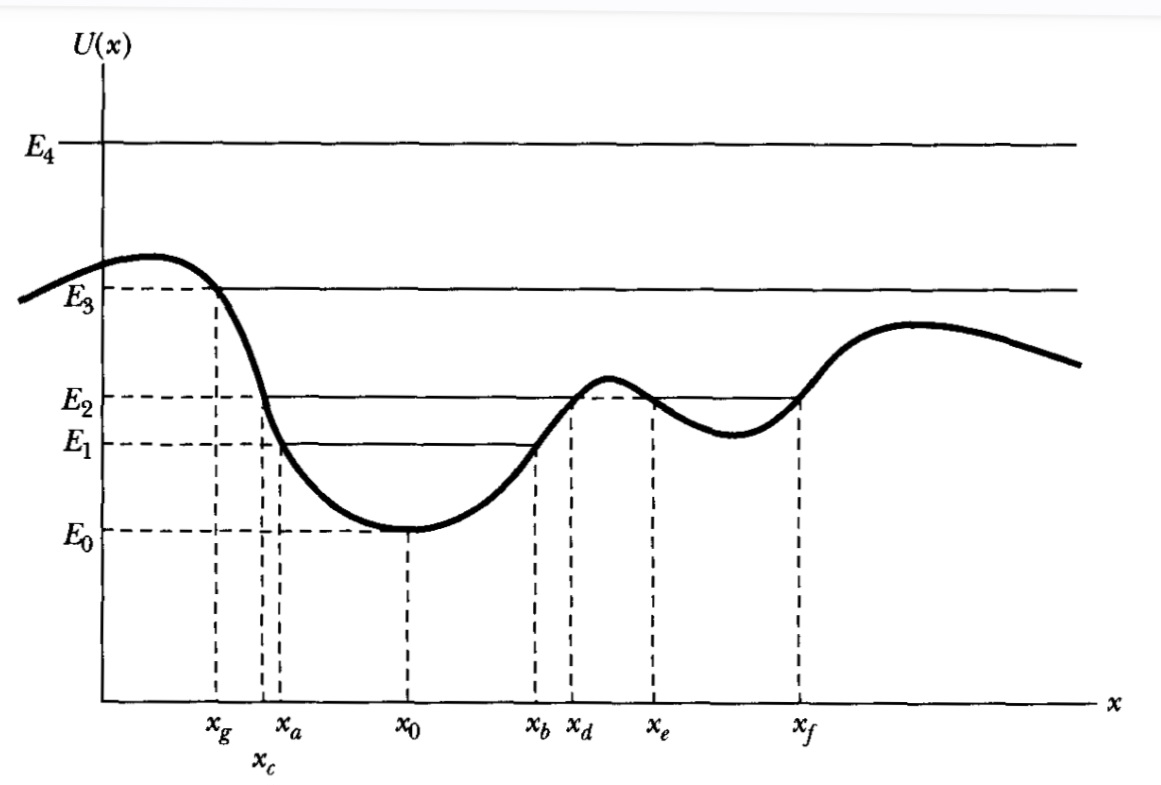
\includegraphics[width=0.7\linewidth]{figure1.1.jpg}
    \caption{물체의 위치에 따른 퍼텐셜 에너지를 그린 그래프이다. $E_0$부터 $E_5$까지 다섯 개의 에너지가 주어져 있으며, 이들과 $U(x)$의 교점 역시 표시되어 있다.}
    \label{fig:1.1}
\end{figure}

그래프를 더욱 자세히 살펴보자. $E_4$의 경우 물체의 위치는 어디든 가능하다. $E_3$의 경우 물체의 위치는 무한정 멀어질 수는 있어도 $x_g$보다 가까워질 수는 없다. $x_g$에 가까이 다가갈수록 속력이 줄어들다가, 마침내 $x_g$에서 0이 되고 말 테니까. $E_2$의 경우 물체의 위치는 $x_c \leq x \leq x_d$와 $x_e \leq x \leq f_d$로 한정되어 있다. 이를 속박되어(bounded) 있다고 표현한다. $E_1$의 경우 물체는 $x_a \leq x \leq x_b$ 사이에 속박되어 있고, $E_0$의 경우 물체의 위치는 $x_0$로 고정되어 있다.

이제 우리는 물체의 총 에너지가 $E_0$에 아주 가까운 경우를 고려한다. 만약 물체의 초기 위치가 $x=x_0$이고 초기 속도는 없다면, 물체는 아무런 힘을 받지 않으므로 계속 그 자리에 있으려 할 것이다. 이렇게 물체에 작용하는 알짜힘이 0인 상태를 \textbf{평형(equlibrium)}이라고 한다. 평형은 안정(stable)할 수도, 불안정(unstable)할 수도, 둘 다 아닐 수도 있다. 평형점에 있던 물체의 위치에 조그마한 변화가 생겼을 때 안정 평형은 물체를 평형점으로 돌아가게 하며, 불안정 평형은 물체를 평형점에서 벗어나게 한다. 비유하자면 골짜기에 놓인 돌은 안정 평형, 산꼭대기에 놓인 돌은 불안정 평형, 평지에 놓인 돌은 둘 다 아닌 경우를 나타내는 셈이다.

평형의 조사는 퍼텐셜 함수의 극값을 조사하는 것과 같다. 매끄러운 함수 $U(x)$에 대해
\begin{equation}
    U(x) = U_0 + x \left(\frac{dU}{dx} \right)_0 + \frac{x^2}{2!} \left(\frac{d^2U}{dx^2} \right)_0 + \frac{x^3}{3!} \left(\frac{d^3U}{dx^3} \right)_0 + \cdots \label{eq:1.32}
\end{equation}
로 전개할 수 있으므로, 만약 $x=x_0$가 평형점이라면
\begin{equation}
    \left(\frac{dU}{dx} \right)_0 = 0 \label{eq:1.33}
\end{equation}
을, $x=x_0$가 안정 평형점이라면
\begin{equation}
    \left(\frac{d^2U}{dx^2} \right)_0 > 0 \label{eq:1.34}
\end{equation}
을, 불안정 평형점이라면
\begin{equation}
    \left(\frac{d^2U}{dx^2} \right)_0 < 0 \label{eq:1.35}
\end{equation}
을 만족한다.

\newpage
% Chapter 2 시작
\chapter{진동 (Oscillations)}

\section{개요}
우리는 앞선 장에서 평형에 관해 배웠다. 1.6절의 상황과 똑같이, 1차원 상에서 운동하는 한 물체를 고려하자. 만약 좌표계의 원점을 평형점으로 정한다면, 물체는 원점을 벗어날 때마다 원점으로 돌아오려는 복원력(restoring force)을 받을 것이다. 복원력 $F$를 테일러 전개로 쓰면
\begin{equation}
    F(x) = F_0 + x \left(\frac{dF}{dx} \right)_0 + \frac{x^2}{2!} \left(\frac{d^2F}{dx^2} \right)_0 + \frac{x^3}{3!} \left(\frac{d^3F}{dx^3} \right)_0 + \cdots \label{eq:2.1}
\end{equation}
이다. 이때 $F_0$는 $x=0$에서 물체가 받는 힘이고, 평형점이므로 그 크기가 0이다.

만약 물체가 평형점으로부터 아주 작은 변위 $x$만큼 움직여 $x^2$과 그 이상의 차수를 무시할 수 있는 경우라면, $k \equiv -(dF/dx)_0$으로 두었을 때 물체가 받는 복원력은
\begin{equation}
    F(x) = -kx \label{eq:2.2}
\end{equation}
가 될 것이다. 익숙하지 않는가? 이것이 바로 \textbf{훅의 법칙(Hooke's Law)}이며, 우리가 이 장에서 다룰 진동의 기본이 된다.

\section{단순 조화 진동 (Simple Harmonic Oscillations)}
훅의 법칙에 따라 진동하는 계, 즉 \textbf{단순 조화 진동자(simple harmonic oscillator)}의 운동 방정식은 식 \ref{eq:2.2}를 $F=ma$로 치환하여 구해진다. 즉,
\begin{equation}
    m\ddot{x} = -kx \label{eq:2.3}
\end{equation}
의 꼴이다. 만약 $\omega^2_0 \equiv k/m$로 정의한다면 위 식은
\begin{equation}
    \ddot{x} + \omega^2_0x = 0 \label{eq:2.4}
\end{equation}
가 된다. 이 미분방정식의 해는 다음과 같다.
\begin{equation}
\begin{aligned}
    x &= A\sin{(\omega_0t-\delta)} \\
    x &= A\cos{(\omega_0t-\phi)} \label{eq:2.5}
\end{aligned}
\end{equation}
이때 $A$는 진폭이며, $\delta$와 $\phi$는 위상각이다. 앞서 운동 방정식을 완벽히 풀기 위해선 초기 조건 2개가 필요하다는 사실을 기억해 보자. 주어진 2개의 조건이 각각 진폭과 위상각의 값을 결정할 것이다.

$\delta$와 $\pi$는 서로 $\pi/2$만큼 차이가 난다. 따라서 식 \ref{eq:2.5}의 첫 번째 줄과 두 번째 줄은 같은 함수를 나타내고 있음에 유의하자.

운동 방정식이 풀렸으므로, 이제 단순 조화 진동에서 발생하는 여러 물리적 관계를 분석할 차례다. 먼저 진동자의 에너지를 구해 보자. $x(t)$를 식 \ref{eq:2.5}의 첫 번째 줄로 두었을 때 진동자의 운동 에너지는
\begin{equation}
    T = \frac{1}{2}m\dot{x}^2 = \frac{1}{2}mA^2\omega_0^2\cos^2{(\omega_0t-\delta)}=\frac{1}{2}kA^2\cos^2{(\omega_0t-\delta)}\label{eq:2.6}
\end{equation}
이고, 퍼텐셜 에너지는
\begin{equation}
    U = -\int Fdx = \int kxdx = \frac{1}{2}kx^2 = \frac{1}{2}kA^2\sin^2{(\omega_0t-\delta)} \label{eq:2.7}
\end{equation}
이므로 총 에너지는
\begin{equation}
    E = T + U = \frac{1}{2}kA^2 \label{eq:2.8}
\end{equation}
이다. 따라서 단순 조화 진동자의 총 에너지는 진폭의 제곱에 비례하며, 시간에 의존하지 않으므로 에너지 보존 법칙이 확인된다.

다음으로 운동의 주기 $\tau_0$는 입자의 위치와 운동 방향이 완전히 같아질 때까지 걸리는 시간 간격으로 정의된다. 식 \ref{eq:2.5}를 분석하면 $\tau_0$는
\begin{equation}
    \omega_0 \tau_0 = 2\pi \label{eq:2.9}
\end{equation}
을 만족해야 함을 알 수 있고, 따라서 주기는
\begin{equation}
    \tau_0 = 2\pi \sqrt{\frac{m}{k}} \label{eq:2.10}
\end{equation}
가 된다. 이때 진동수 $f$는
\begin{equation}
    f = \frac{1}{\tau_0}=\frac{1}{2\pi}\sqrt{\frac{k}{m}} \label{eq:2.11}
\end{equation}
이고, 각진동수은 $\omega_0$이다. 주기가 진폭에 의존하지 않는다는 사실을 기억하자.

\begin{examplebox}{예제 2.1}
\begin{example}
단진자는 단순 조화 진동자의 대표적인 예시이다. 길이가 $l$인 실에 질량이 $m$인 추가 달려 있다고 가정하자. 추가 평형점에서 아주 작은 각도 $\theta$만큼 기울어져 있을 때, 단진자의 주기를 구하여라.
\end{example}
\end{examplebox}

\begin{solution}
    우리는 실의 질량과 추의 크기를 무시한다. 자유물체도를 그려보자. 공에 작용하는 힘은 중력 $mg$와 장력이며, 실이 늘어나거나 줄어들지 않으므로 장력의 크기는 $mg\cos{\theta}$이다. 따라서 진자 운동에 기여하는 힘은 $mg\sin{\theta}$의 크기를 가지며 회전각 $\theta$를 줄이려는 방향으로 작용하는 중력 분력이다. 이제 토크를 분석하자. 앞선 논의에 따라 추에 작용하는 토크는 $-mgl\sin{\theta}$이다. 토크는 관성 모멘트와 각가속도의 곱으로 나타낼 수 있고, 추의 관성 모멘트는 $ml^2$이므로, 운동 방정식은
    \begin{equation}
        ml^2\ddot{\theta}=-mgl\sin{\theta} \label{eq:2.12}
    \end{equation}
    이 된다. $\theta$의 크기가 아주 작으므로 $\sin{\theta} \approx \theta$처럼 근사하고 양변을 정리하면
    \begin{equation}
        \ddot{\theta} + \frac{g}{l}\theta = 0 \label{eq:2.13}
    \end{equation}
    이다. 이는 단순 조화 진동자의 운동 방정식이므로, 식 \ref{eq:2.10}을 통해 주기를 구하면
    \begin{equation}
        \tau_0=2\pi \sqrt{\frac{l}{g}} \label{eq:2.14}
    \end{equation}
    을 얻는다. 주기는 실의 길이 $l$에 의존하며 추의 질량 $m$에는 의존하지 않는다.
\end{solution}

\noindent\rule{\textwidth}{0.8pt} % 본문 전체 너비만큼 0.8pt 두께의 검은 줄을 긋습니다.
\vspace{1em} % 줄 아래에 약간의 여백을 줍니다.

이제 우리는 단순 조화 진동을 2차원 상으로 확장해 보려고 한다. 원점을 평형점으로 잡고 물체의 위치벡터를 $\textbf{r}$이라고 하면, 물체에 작용하는 복원력은 $\textbf{F} = -k\textbf{r}$이 될 것이다. 이를 직교 좌표계의 각 성분별로 쓰면
\begin{equation}
    \begin{aligned}
       F_x &= -kx \\ F_y &= -ky \label{eq:2.15}
    \end{aligned}
\end{equation}
이 된다. 따라서 운동 방정식은
\begin{equation}
\begin{aligned}
    \ddot{x} + \omega^2_0x &= 0 \\
    \ddot{y} + \omega^2_0y &= 0 \label{eq:2.16}
\end{aligned}
\end{equation}
이고, 이 운동 방정식의 해는
\begin{equation}
\begin{aligned}
    x(t) &= A\cos{(\omega_0t-\alpha)} \\
    y(t) &= B\cos{(\omega_0t-\beta)} \label{eq:2.17}
\end{aligned}
\end{equation}
이다. 결과적으로 물체는 두 방향으로 단순 조화 진동을 하며, 두 진동은 서로 같은 진동수를 가지지만 초기 조건에 따라 진폭과 위상은 다를 수 있다.

한편 우리는 식 \ref{eq:2.17}에서 시간 $t$를 소거하여 물체의 궤적을 2차원 평면 상으로 나타낼 수 있다. 즉,
\begin{equation}
\begin{split}
    y(t) &= B\cos{[\omega_0t-\alpha+(\alpha-\beta)]} \\ 
         &= B\cos{(\omega_0t-\alpha)}\cos{(\alpha-\beta)}-B\sin{(\omega_0t-\alpha)}\sin{(\alpha-\beta)}
\end{split}
\label{eq:2.18}
\end{equation}
처럼 쓰고 $\delta \equiv \alpha-\beta$로 둔 다음 $\cos{(\omega_0t-\alpha)}=x/A$로 치환하면
\begin{equation}
    y = \frac{B}{A}x\cos{\delta} - B\sqrt{1-\frac{x^2}{A^2}}\sin{\delta} \label{eq:2.19}
\end{equation}
를 얻는다. 이때 $\delta=0$이면
\begin{equation}
    y = \frac{B}{A}x \label{eq:2.20}
\end{equation}
인 직선이, $\delta=\pm\pi$라면
\begin{equation}
    y = -\frac{B}{A}x \label{eq:2.21}
\end{equation}
인 직선이,
$\delta=\pm\pi/2$라면
\begin{equation}
    \frac{x^2}{A^2} + \frac{y^2}{B^2} = 1 \label{eq:2.22}
\end{equation}
인 타원이 나온다. 특히 식 \ref{eq:2.22}에서 $A=B$라면 물체의 궤적은 원이다. $A=B$를 만족하는 경우, 몇 가지 $\delta$값에 따른 물체의 궤적이 그림 \ref{fig:2.1}에 그려져 있다.

\begin{figure}
    \centering

 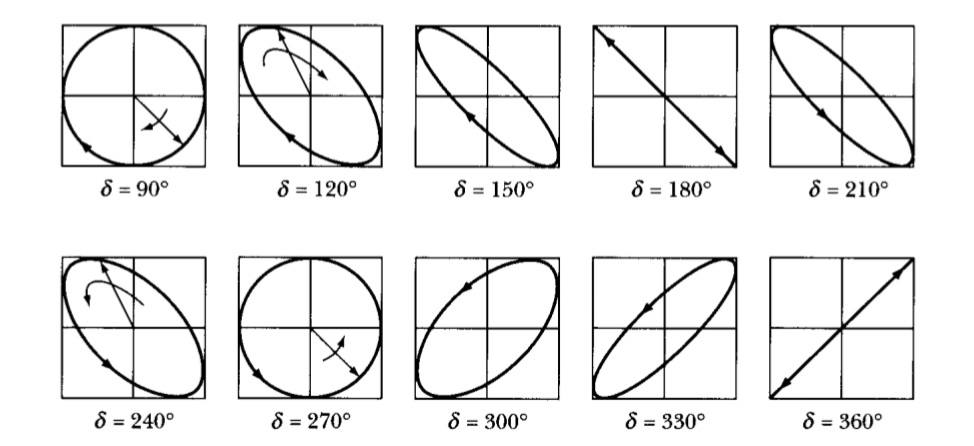
\includegraphics[width=0.7\linewidth]{figure2.1.jpg}
    \caption{2차원 단순 조화 운동을 나타낸 그림이다. $\delta=\alpha-\beta$와 $A=B$를 가정했다.}
    \label{fig:2.1}
\end{figure}

보다 일반적으로, 2차원 단순 조화 진동에서 물체의 $x$ 방향과 $y$ 방향에 작용하는 복원력은 서로 다를 수 있다. 복원력이 달라지면 각진동수 역시 달라진다. 이때 물체의 궤적은 더이상 타원의 형태를 띠지 않고 \textbf{리사주 곡선(Lissajous curve)}을 그린다. 리사주 곡선은 두 방향의 각진동수 $\omega_x$와 $\omega_y$가 정수비를 이룰 경우 닫힌 곡선, 그렇지 않으면 열린 곡선이다.\footnote{어떠한 운동이 일정한 시간 간격으로 반복된다면 그 운동이 그리는 곡선은 닫힌 곡선(closed curve)이고, 무한한 시간이 지나도 특정 운동이 반복되지 않는다면 열린 곡선(open curve)이다.} 닫힌 곡선의 경우 물체는 주기적으로 운동하며 그림 \ref{fig:2.2}와 같이 기하학적인 궤적을 그리고, 열린 곡선의 경우 물체는 한 지점을 같은 속도로 지나치지 않으며 $2A \times 2B$의 직사각형을 가득 채워 나가는 궤적을 그린다.

\begin{figure}
    \centering

 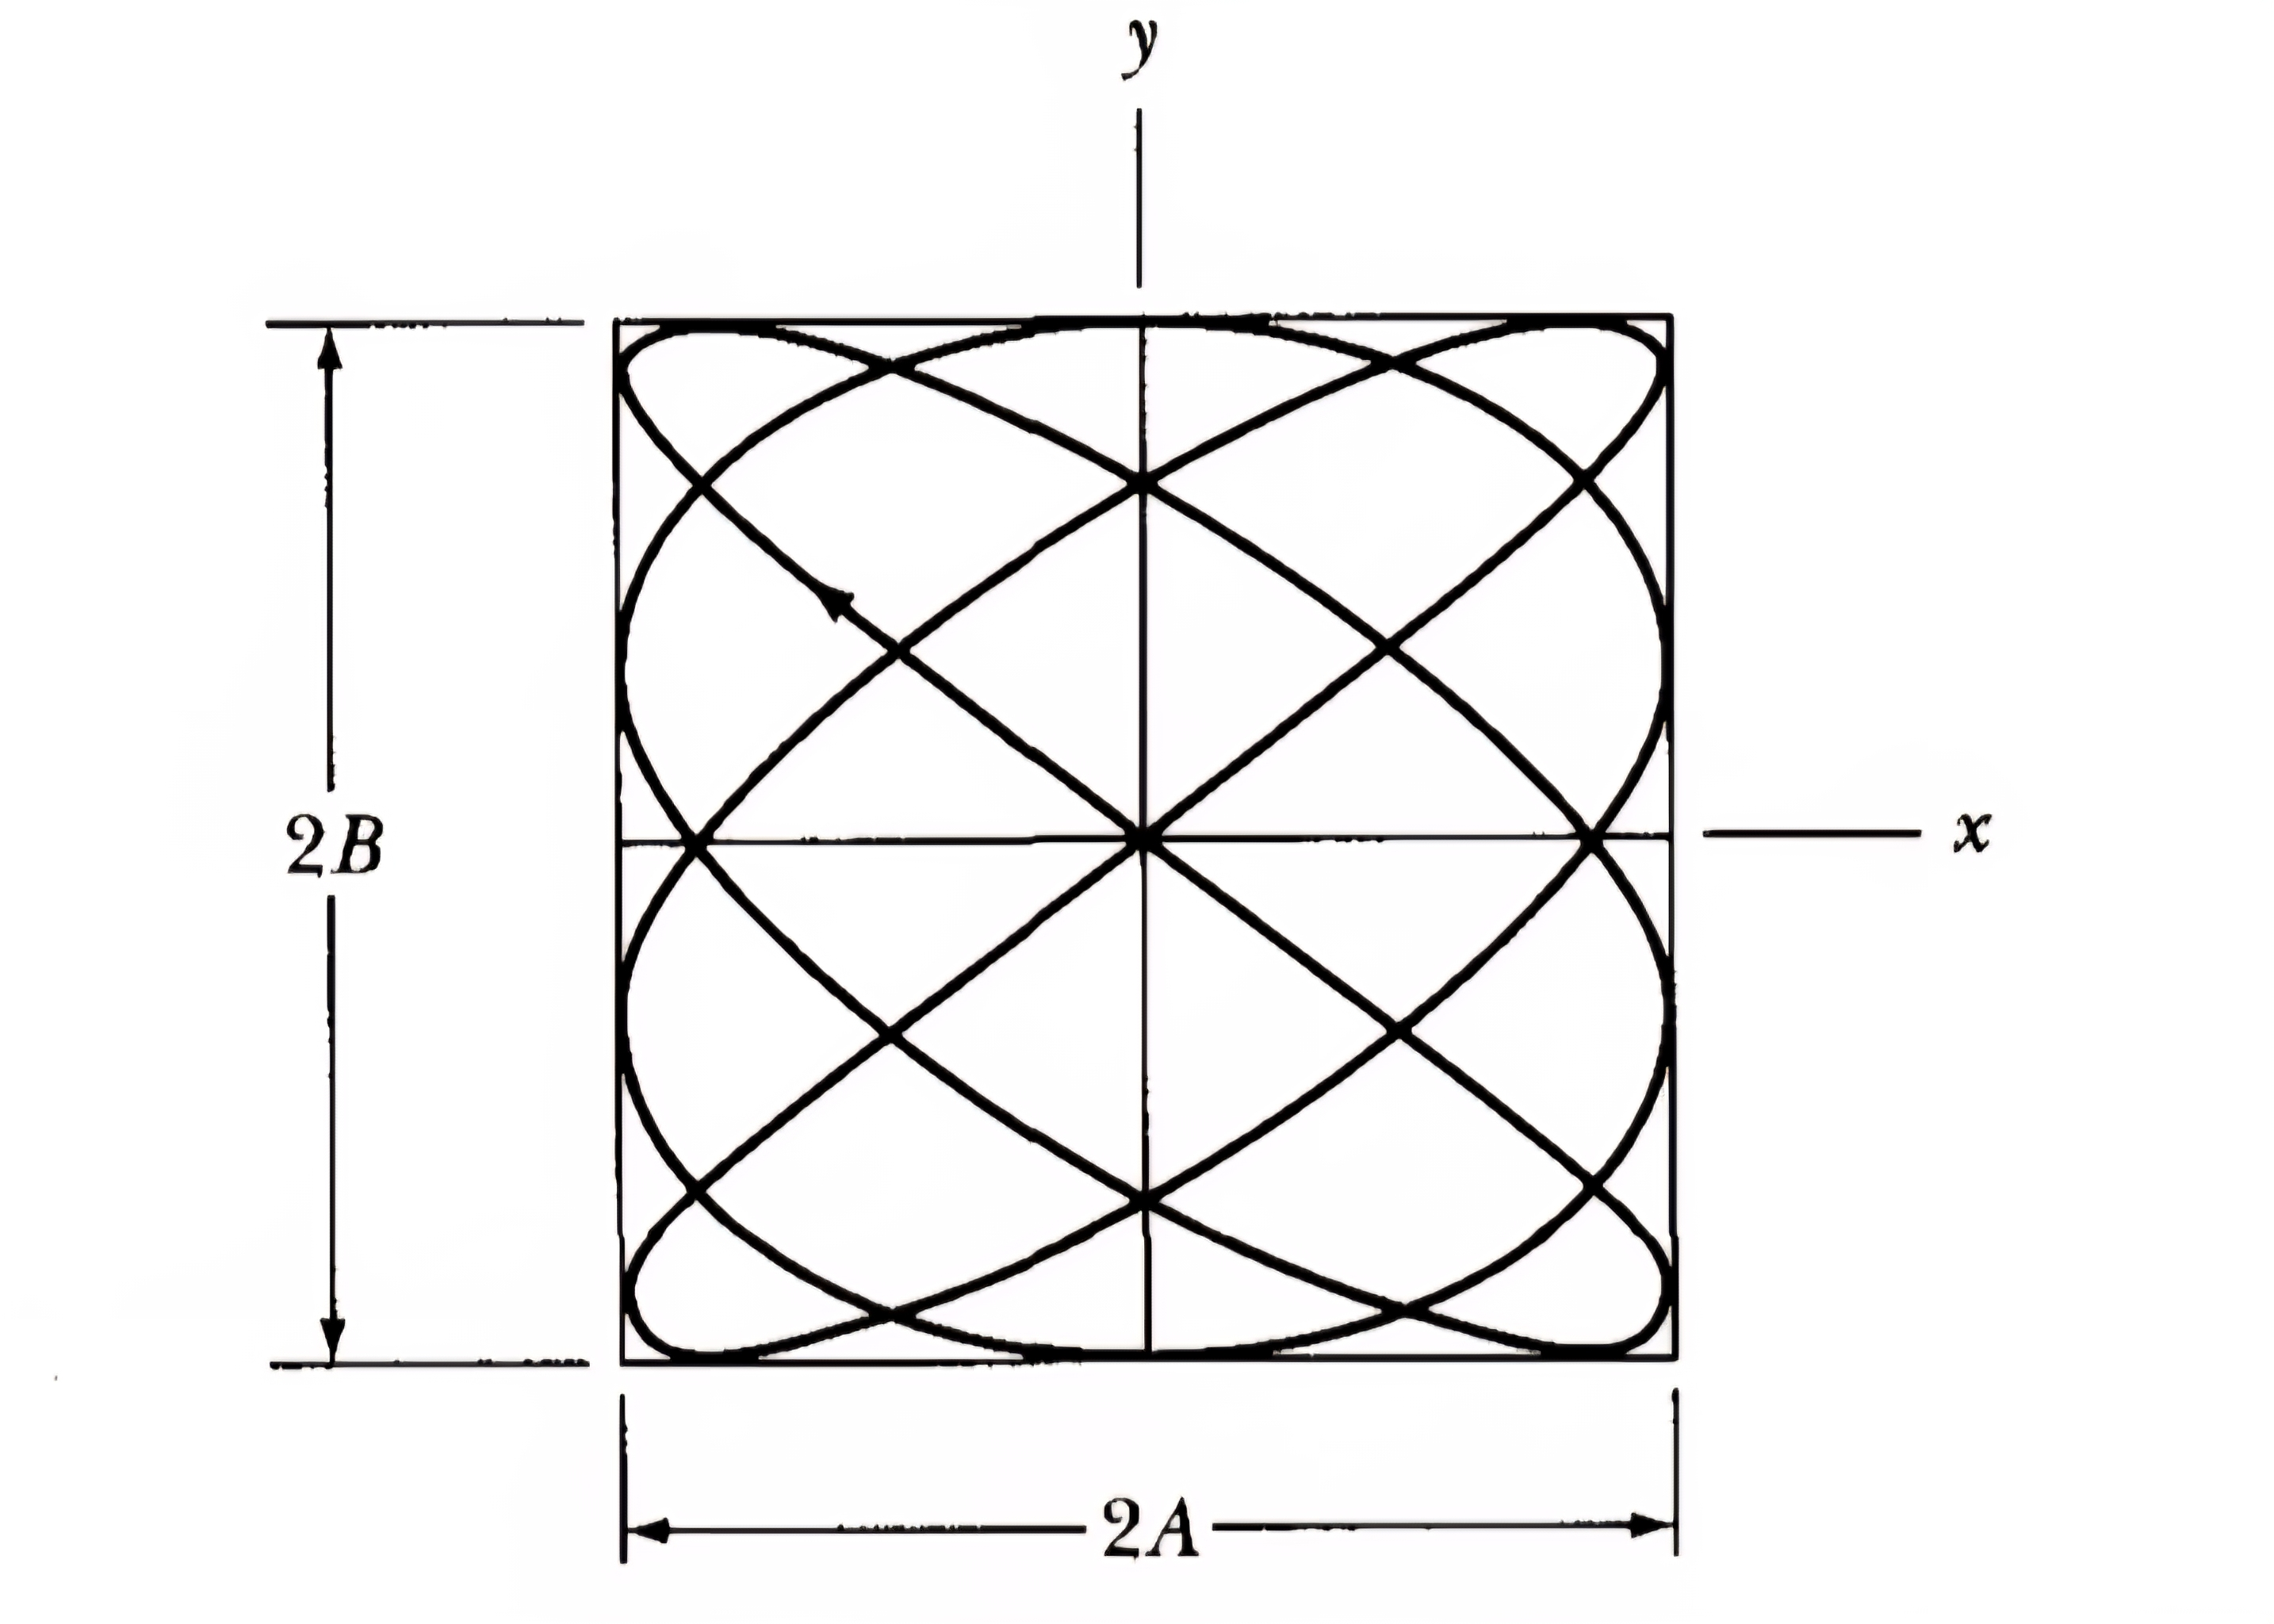
\includegraphics[width=0.7\linewidth]{figure2.2.jpg}
    \caption{리사주 곡선의 한 예시이다. $\omega_x$와 $\omega_y$의 비는 $4:3$이다.}
    \label{fig:2.2}
\end{figure}

\section{위상도 (Phase Diagrams)}
앞선 절에서 우리는 단순 조화 진동에 대해 분석했다. 1차원으로 한정하면, 단순 조화 진동하는 물체의 시간에 따른 위치는 식 \ref{eq:2.5}와 같다. 여기서 우리가 모르는 물리량은 진폭과 위상각이다. 따라서 물체의 운동을 완벽히 분석하기 위해선 조건 2개가 더 필요하다. 우리는 이 조건을 초기 위치와 초기 속도에서 찾는다.

그렇다면 이건 어떨까? 우리는 위치와 속도를 축으로 하는 2차원 공간을 생각해볼 수 있다. 이를 \textbf{위상 공간(phase space)}이라고 한다.\footnote{정확히 말하자면, 자유도가 $n$인 물체의 위상 공간은 $2n$차원이다. 지금 우리는 1차원 상에서의 단순 조화 운동을 분석하고 있기에 위상 공간이 2차원인 것이다.} 물체가 운동한다면, 위상 공간 위의 점 $P(x(t), \dot{x}(t))$는 시간에 따라 어떠한 궤적을 그릴 것이다. 초기 조건이 달라지면 이 궤적 역시 달라지므로, 궤적은 초기 조건에 대응한다.
이렇게 위상 공간에 그려지는 물체의 궤적이 바로 \textbf{위상도(phase diagram)}이다.

앞서 다루었던 단순 조화 진동을 예시로 들자. 식 \ref{eq:2.5}의 첫 번째 줄을 활용하면 물체의 위치와 속도는 각각
\begin{equation}
\begin{split}
    x(t) &= A\sin{(\omega_0t-\delta)} \\
    \dot{x}(t) &= \omega_0A\cos{(\omega_0t-\delta)} \label{eq:2.23}
\end{split}
\end{equation}
이므로, 시간 $t$를 소거하면
\begin{equation}
    \frac{x^2}{A^2} + \frac{\dot{x}^2}{A^2\omega^2} = 1 \label{eq:2.24}
\end{equation}
을 얻는다. 즉 위상 공간 상에서 단순 조화 진동의 궤적은 타원이다. 식 \ref{eq:2.8}을 이용하면 이 타원의 방정식은
\begin{equation}
    \frac{x^2}{2E/k} + \frac{\dot{x}^2}{2E/m} = 1 \label{eq:2.25}
\end{equation}
처럼 바꾸어 쓸 수 있다. 따라서 각 타원 궤도는 진동자의 총 에너지에 대응한다.

위상 공간 상에서 단순 조화 진동의 궤적은 서로 겹치지 않는다. 만약 겹친다면 교차점 $P(x(t), \dot{x}(t))$를 초기 조건으로 하는 진동자는 두 가지 운동 상태를 가져야 할 것이다. 하지만 초기 조건 2개가 주어질 때 진동자의 운동 방정식의 해는 유일하므로 이는 불가능하다.

위상 공간은 초기 조건에 따른 물체의 운동 상태를 쉽게 알아볼 수 있다는 점에서 유용하다. 우리는 앞으로 이 마법진 같은 개념을 다양한 곳에 활용할 것이다.

\section{감쇠 조화 진동 (Damped Harmonic Oscillations)}
2.2절에서 보았던 단순 조화 진동자는 이상적인 상황을 가정했을 때 나온 결과물이다. 공기 저항이 없어 한 번 진동을 시작하면 영원히 멈추지 않으니까. 따라서 우리는 항력과 같은 \textbf{감쇠력(damping force)}이 존재하는, 보다 현실적인 계인 \textbf{감쇠 조화 진동자(damped harmonic oscillator)}를 다루고자 한다.

일반적으로 항력은 물체의 속도에 비례한다. 우리는 여전히 1차원 운동만을 분석할 것이므로 항력을 $F=-b\dot{x}$로 쓸 수 있다. 항력의 방향은 물체의 운동과 반대 방향이므로 $b>0$이다. 이때 운동 방정식은 다음과 같다.
\begin{equation}
    m\ddot{x}+b\dot{x}+kx=0 \label{eq:2.26}
\end{equation}

이제 이 운동 방정식을 풀어보자. 위 식은 2계 선형 제차 미분방정식이다. 이 경우 해가 만족하는 성질은 크게 세 가지가 있다. 먼저 $x_1$이 해이면 $x_1$의 복소수 상수 배인 $A_1x_1$도 해이다. 다음으로 $x_1, x_2$가 해이면 $x_1+x_2$도 해이다. 마지막으로 $x_1, x_2$가 서로 선형 독립인 해이면 방정식의 일반해는 $A_1x_1+A_2x_2$가 된다.\footnote{첫 번째 성질과 두 번째 성질은 미분이 선형 연산이기 때문에 성립한다. 세 번째 성질은 이 미분방정식의 일반해가 $x_1$과 $x_2$의 선형 결합이 되어야 한다는 것인데, 대수학적으로 보면 이 미분방정식을 만족하는 해들이 이루는 공간(해공간)은 2차원 벡터 공간과 구조가 완전히 같다. 2차원 평면을 빈틈없이 전부 표현하려면 선형 독립인 기저 벡터 2개가 필요한 것처럼, 2계 미분방정식의 2차원 해공간을 전부 표현하려면 서로 선형 독립인 해 2개가 필수적이다. 만약 $x_1$과 $x_2$가 선형 독립이라면 이 둘은 해공간의 기저 역할을 맡게 되고, 따라서 미분방정식의 그 어떤 해를 가져오더라도 기저의 결합인 $A_1x_1 + A_2x_2$의 형태로 모두 표현할 수 있게 되므로 이는 일반해가 된다.}

계산의 편의를 위해 식 \ref{eq:2.26}을
\begin{equation}
    \ddot{x}+2\beta\dot{x}+\omega_0^2x=0 \label{eq:2.27}
\end{equation}
과 같이 변형하자. 즉, $\beta \equiv b/2m$이다. $\beta$는 \textbf{감쇠 계수(damping coefficient)}라고 불리며 계에 얼마만큼의 감쇠력이 존재하는지를 나타낸다. 우리는 식 \ref{eq:2.27}의 해를 $x=e^{rt}$로 가정\footnote{이처럼 해의 꼴을 그럴듯하게 가정해 놓고 문제를 푸는 방식을 ansatz라고 한다.}하여 다음과 같은 특성 방정식(characteristic equation)\footnote{혹은 보조 방정식(auxiliary equation)이라고도 한다.}을 얻는다.
\begin{equation}
    r^2+2\beta r + \omega_0^2 = 0 \label{eq:2.28}
\end{equation}
이 이차방정식의 해는 $r = -\beta \pm \sqrt{\beta^2-\omega_0^2}$이므로, 2계 선형 제차 미분방정식의 성질에 따라 식 \ref{eq:2.27}의 일반해는
\begin{equation}
    x(t) = e^{-\beta t}[A_1e^{\sqrt{\beta^2-\omega_0^2}t}+A_2e^{-\sqrt{\beta^2-\omega_0^2}t}] \label{eq:2.29}
\end{equation}가 된다. $A_1$과 $A_2$는 초기 조건이 주어질 때 비로소 결정될 것이다.

식 \ref{eq:2.29}는 $\beta^2 < \omega_0^2$인 경우, $\beta^2 = \omega_0^2$인 경우, 그리고 $\beta^2 > \omega_0^2$인 경우에 따라 그 형태가 크게 달라진다. 그림 \ref{fig:2.3}을 참고하라. 각각의 경우에 대응하는 물체의 운동은 underdamped motion, critically damped motion, overdamped motion이다. 우리는 세 운동을 차례대로 분석해 볼 것이다.

\begin{figure}
    \centering

 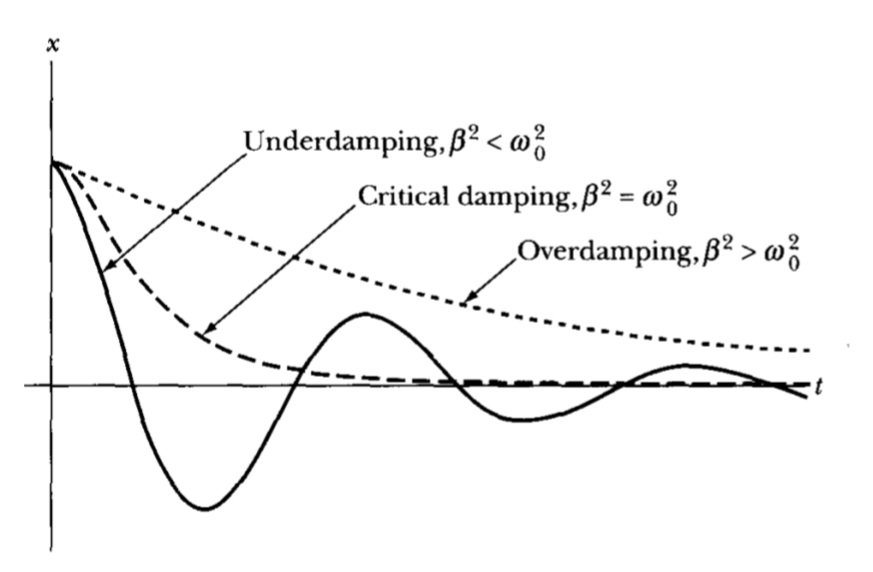
\includegraphics[width=0.7\linewidth]{figure2.3.jpg}
    \caption{특정 초기 조건 하에서 감쇠 조화 진동하는 물체의 운동이다.}
    \label{fig:2.3}
\end{figure}

먼저 $\beta^2 < \omega_0^2$인 경우를 보자. 편의를 위해 $\omega_1^2 \equiv \omega_0^2-\beta^2$을 도입하면 운동 방정식의 해는
\begin{equation}
    x(t) = e^{-\beta t}[A_1e^{i\omega_1t}+A_2e^{-i\omega_1t}] \label{eq:2.30}
\end{equation}가 된다. 이때 실제 위치를 나타내는 물리량 $x(t)$는 실수여야 하므로, 켤레복소수가 자신과 같다는 조건을 만족해야 한다. 즉,
\begin{equation}
    \overline{x(t)} = e^{-\beta t}[\overline{A_1} \cdot \overline{e^{i\omega_1t}} + \overline{A_2} \cdot \overline{e^{-i\omega_1t}}] \label{eq:2.31}
\end{equation}
가 $x(t)$와 동일해야 한다. 오일러 공식을 적용하면
\begin{equation}
    \overline{e^{i\omega_1t}} = \overline{\cos{\omega_1t}+i\sin{\omega_1t}} = \cos{\omega_1t} - i\sin{\omega_1t} = e^{-i\omega_1t} \label{eq:2.32}
\end{equation}
가 성립하므로 식 \ref{eq:2.31}은
\begin{equation}
    \overline{x(t)} = e^{-\beta t}[\overline{A_1}e^{-i\omega_1t} + \overline{A_2}e^{i\omega_1t}] \label{eq:2.33}
\end{equation} 처럼 쓸 수 있다. 이를 식 \ref{eq:2.30}과 비교하면 $\overline{A_1}=A_2$, $\overline{A_2}=A_1$을 얻는다. 이 조건을 만족하도록 임의의 실수 $a$, $b$, $\delta$를 도입하여 $A_1 \equiv a-bi, A_2 \equiv a+bi$, $A \equiv 2\sqrt{a^2 + b^2}$로 두면
\begin{equation}
\begin{split}
    A_1 &= \sqrt{a^2+b^2}(\cos{\delta}-i\sin{\delta}) = \frac{A}{2} e^{-i\delta} \\
    A_2 &= \sqrt{a^2+b^2}(\cos{\delta}+i\sin{\delta}) = \frac{A}{2} e^{i\delta} \label{eq:2.34}
\end{split}
\end{equation}
이고, 이를 식 \ref{eq:2.30}에 대입하여
\begin{equation}
    x(t) = \frac{A}{2} e^{-\beta t}[e^{-i(\omega_1t-\delta)}+e^{i(\omega_1t-\delta)}] \label{eq:2.35}
\end{equation}
를 얻는다. $2\cos{(\omega_1-\delta t)}=e^{i(\omega_1-\delta t)}+e^{-i(\omega_1-\delta t)}$이므로, 해는 결국
\begin{equation}
    x(t) = A e^{-\beta t}\cos{(\omega_1t-\delta)} \label{eq:2.36}
\end{equation}
가 된다.

Underdamped motion의 운동 방정식을 풀었으므로 이제 분석할 차례다. 우리는 종종 $\omega_1$을 감쇠 조화 진동자의 각진동수라고 부르지만, 이는 엄밀히 말하면 잘못된 표현이다. $x(t)$의 꼴을 보면 알겠지만 감쇠 조화 진동자의 운동은 비주기적이기 때문이다. 하지만 물체는 $x=0$을 주기적으로 지나치고, 이 시간 간격을 $T_1$이라고 하면 $\omega_1=2\pi/2T_1$이 성립하므로 우리는 $\omega_1$을 각진동수처럼 생각할 수 있다.

$\omega_1$에 대해 조금 더 알아보자. 감쇠력이 존재한다면 $\omega_1$은 단순 조화 진동자의 각진동수 $\omega_0$보다 항상 작다. $\beta>0$에 대해 $\omega_1^2 \equiv \omega_0^2-\beta^2$이기 때문이다. 따라서 감쇠 조화 진동하는 물체는 $x=0$을 지나치는 시간 간격($T_1$)이 단순 조화 진동하는 물체의 시간 간격보다 더 길다.

한편 감쇠 조화 진동자의 진폭을 결정하는 항은 $Ae^{-\beta t}$이다. 이는 시간에 따라 지수적으로 감소한다. 따라서 우리는 충분한 시간이 흐른 뒤 물체가 평형점 근처에 머물러 있을 것임을 유추할 수 있다. 어떻게 이런 일이 일어날 수 있을까? 진동자의 총 에너지가 감소하기 때문이다. 항력은 보존력이 아니므로 계의 총 에너지는 시간이 흐르며 감소한다. 즉,
\begin{equation}
    E = T+U=\frac{1}{2}m\dot{x}^2+\frac{1}{2}kx^2 \label{eq:2.37}
\end{equation}
의 양변을 시간 $t$로 미분하면
\begin{equation}
    \frac{dE}{dt} = m\dot{x}\frac{d\dot{x}}{dt}+kx\frac{dx}{dt} = m\dot{x}\ddot{x} + kx\dot{x} = \dot{x}(m\ddot{x}+kx) = -b\dot{x}^2 \label{eq:2.38}
\end{equation}
이므로, 감쇠 조화 진동자의 총 에너지는 속도의 제곱에 비례하여 감소한다.

에너지 감소를 보다 시각적으로 확인하기 위해 앞선 절에서 배운 위상도를 그려 보자. 식 \ref{eq:2.36}을 시간에 대해 미분하면
\begin{equation}
    \dot{x}(t) = -Ae^{-\beta t}[\omega_1\sin{(\omega_1t-\delta)}+\beta \cos{(\omega_1t-\delta)}] \label{eq:2.39}
\end{equation}
이므로, 우리는 $x(t)$와 $\dot{x}(t)$의 관계를 조사하여 위상도를 그릴 수 있다. 그 결과는 그림 \ref{fig:2.4}와 같은 나선이다. 나선의 중심점, 즉 위상도의 궤적이 향하는 곳은 \textbf{끌개(attractor)}라는 이름이 있다. 에너지가 감소하는 경우 위상도는 그렇지 않을 때와 명백히 다른 모습을 보인다.

\begin{figure}
    \centering

 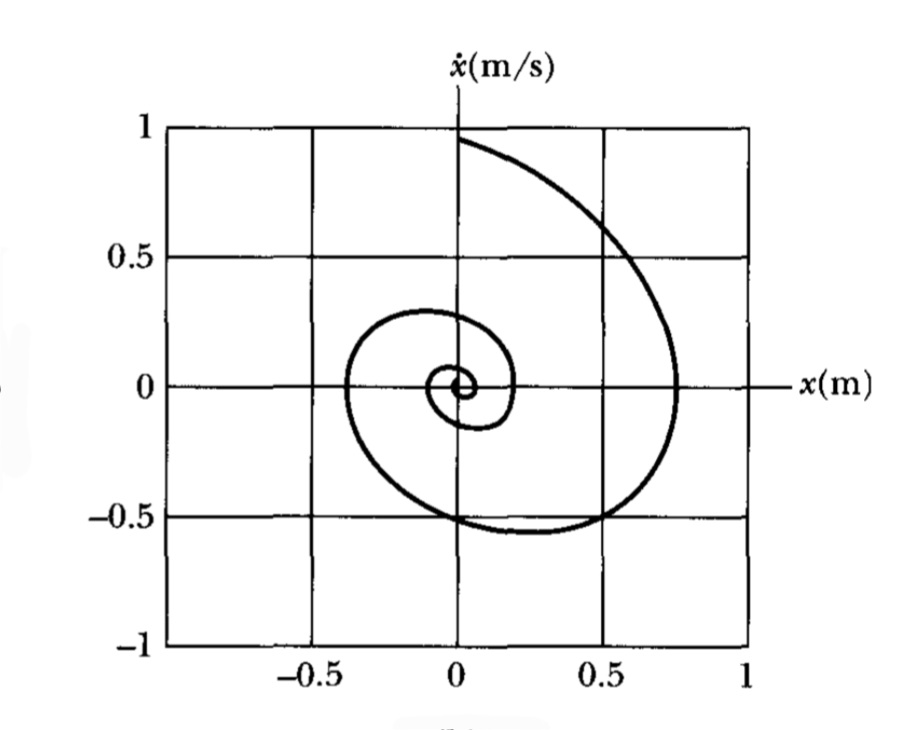
\includegraphics[width=0.7\linewidth]{figure2.4.jpg}
    \caption{Underdamped motion의 위상도이다. $A=1$ cm, $\omega_0=1$ rad/s, $\beta=0.2$ 1/s, 그리고 $\delta=\pi/2$를 가정했다.}
    \label{fig:2.4}
\end{figure}

이제 식 \ref{eq:2.29}로 돌아가 $\beta^2=\omega_0^2$인 경우를 보자. 정성적으로 생각해볼 때, 감쇠력이 충분히 크다면 물체의 운동은 진동의 형태를 띠지 않고 빠르게 $x=0$으로 수렴할 것이다. $\beta^2=\omega_0^2$은 물체가 더는 진동하지 않게 되는 임계(critical) 조건이며, 그래서 우리는 이 경우를 특별히 critically damped motion이라고 부른다.

Critically damped motion의 운동 방정식을 풀어 보자. 이 경우, 특성 방정식인 식 \ref{eq:2.28}은 $(r+\beta)^2=0$이 되어 중근을 가진다. 여기서 문제가 생긴다. 알고 있는 해가 $e^{rt}$ 하나이기 때문에 2계 선형 제차 미분방정식의 해의 성질을 이용할 수 없다는 것이다! 다행히도 고대의 대마법사들은 이 문제를 이미 해결해 놓았다. 우리는 미분방정식의 해공간의 기저를 $e^{rt}$와 $te^{rt}$로 놓을 수 있다.\footnote{자연수 n과 복소수 c에 대해, $(r-c)^n$이 계수가 상수인 선형 동차 미분방정식의 특성 방정식이라면 $e^{ct}$, $te^{ct}, t^2e^{ct}... t^{n-1}e^{ct}$은 모두 미분방정식의 해공간의 기저가 된다. 구체적인 증명은 Friedberg 교재를 참고하라.} 이제 해의 성질을 이용하면 식 \ref{eq:2.27}의 일반해는
\begin{equation}
    x(t) = e^{-\beta{t}}(A_1+A_2t) \label{eq:2.40}
\end{equation}
가 된다.

그림 \ref{fig:2.3}에서 볼 수 있듯, 식 \ref{eq:2.40}은 정말로 진동하지 않고 $x=0$으로 수렴한다. 특기할 만한 점은 critically damped motion의 수렴 속도가 다른 운동에 비해 가장 빠르다는 점이다. 따라서 이 운동은 충격을 받았을 때 요동치지 않고 곧바로 제자리에 정지할 필요가 있는 자동차의 충격 흡수 장치 등에 활용된다.

마지막으로 식 \ref{eq:2.29}에서 $\beta^2>\omega_0^2$인 경우를 보자. $\omega_2=\sqrt{\beta^2-\omega_0^2}$을 도입하면
\begin{equation}
    x(t) = e^{-\beta t}[A_1e^{\omega_2t}+A_2e^{-\omega_2t}] = A_1e^{-(\beta-\omega_2)t}+A_2e^{-(\beta+\omega_2)t}\label{eq:2.41}
\end{equation}
가 된다. 이때 우리는 $\omega_2$를 각진동수라고 부르지 않는다. 주기적인 운동이 전혀 없기 때문이다. 그림 \ref{fig:2.3}에서 보았듯 overdamped motion을 겪는 물체는 $x=0$을 향해 점근적으로 다가갈 뿐이다.

\begin{figure}
    \centering

 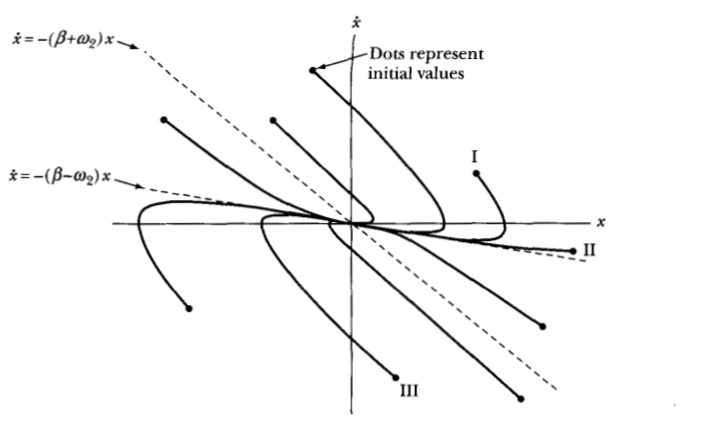
\includegraphics[width=0.7\linewidth]{figure2.5.jpg}
    \caption{다양한 초기 조건에 따른 Overdamped motion의 위상도이다.}
    \label{fig:2.5}
\end{figure}

다만 overdamped motion은 초기 조건에 따라 형태가 더욱 복잡해질 수 있다. 위상도를 통해 이를 자세히 분석하자. 그림 \ref{fig:2.5}는 세 가지 초기 조건 I, II, III에 따른 overdamped motion의 위상도이다. 먼저 공통적인 사항으로, 위상도 상의 궤적은 초기 조건에 관계없이 시간이 흐름에 따라 직선 $\dot{x}=-(\beta-\omega_2)x$에 가까워지는 모습을 보인다. 식 \ref{eq:2.41}은 두 항으로 이루어지는데, $t$가 커질수록 $A_1$ 항이 $A_2$ 항보다 우세해지기 때문이다. 이를 수식으로 설명하자면
\begin{equation}
\begin{split}
    x(t) &= A_1 e^{-(\beta-\omega_2)t} + A_2e^{-(\beta+\omega_2)t} \\ \dot{x}(t) &= -A_1 (\beta - \omega_2) e^{-(\beta-\omega_2)t} - A_2 (\beta+\omega_2)e^{-(\beta+\omega_2)t} \label{eq:2.42}
\end{split}
\end{equation}
에서 두 식의 $A_2$ 항을 모두 0으로 근사한 경우로 볼 수 있다.

초기 조건 I, II, 그리고 III을 개별적으로 분석해 보자. 먼저 조건 I은 초기 위치와 초기 속도가 모두 양수이다. 진동자에는 복원력이 작용하므로, 초기 속도는 점점 줄어들다가 음수로 바뀐다. 반면 위치는 계속 양수를 유지하고, 물체는 $x=0$에 도달한 뒤 감쇠력에 의해 모든 에너지를 잃고 정지한다. 기본적인 형태는 그림 \ref{fig:2.4}의 나선과 같지만, 중심으로 휘말리는 정도가 더 심하다고 이해하면 좋다.

다음으로 조건 II는 초기 위치는 양수, 초기 속도는 음수인 경우이다. 이 경우 물체는 이미 종착점인 $x=0$을 향해 가고 있으므로, 위치와 속도의 부호 변화 없이 원점에 도달하여 정지한다.

마지막으로 조건 III은 조금 특별하다. 조건 II와 같이 초기 위치는 양수이고 초기 속도는 음수이지만, 속력이 너무 큰 나머지 물체는 종착점 $x=0$을 지나 위치가 음수인 영역까지 도달한다. 이후 속도의 부호가 양수로 바뀌고, 종착점인 $x=0$에 도달하여 정지한다. 이 경우 물체는 최종 상태에 도달하기 전까지 $x=0$을 한 번 지나치므로 관점에 따라선 진동한다고 볼 수도 있다. 하지만 운동 과정에서 물체가 강한 감쇠력을 받고, 그로 인해 종착점에 빠르게 도달한다는 사실은 분명하다.

우리는 이렇게 감쇠 조화 진동에서 나타나는 세 가지 형태의 운동을 조사했다. 운동의 분석 과정은 언뜻 보면 복잡할 수 있지만, 운동 방정식을 세우고 푼다는 기본 원리는 같다. 여기에 위상도를 얹혀 초기 조건의 변화에 따른 움직임을 살핀다면 금상첨화. 사실, 고전역학이라는 마법을 다루는 과정은 이제 시작이다.

\section{사인형 구동력 (Sinusoidal Driving Forces)}
많은 경우 우리는 조화 진동자에 외부 힘이 작용하는 상황을 다룰 필요가 있다. 가장 흔한 예시는 일정한 주기로 그네를 밀어 주는 경우이다. 이처럼 외부 힘이 시간에 따른 함수 $F(t)$로 주어진다면 계의 운동 방정식은 다음과 같다.
\begin{equation}
    m\ddot{x}+b\dot{x}+kx=F(t) \label{eq:2.43}
\end{equation}
우리는 이러한 운동 방정식을 가지는 계를 \textbf{강제 조화 진동자(driven harmonic oscillator)}라고 부르며, 이때 $F(t)$는 진동자의 \textbf{구동력(driving force)}이 된다.

가장 일반적인 형태의 구동력은 사인형 구동력이다. 즉, 구동력이 $F=F_0\cos{\omega t}$의 꼴인 경우이다. 따라서 운동 방정식은
\begin{equation}
    m\ddot{x} + b\dot{x}+kx=F_0\cos{\omega t} \label{eq:2.44}
\end{equation}
이며, $\beta \equiv b/2m$, $\omega_0 \equiv \sqrt{k/m}$, $A \equiv F_0/m$를 도입하면 이 식은
\begin{equation}
    \ddot{x} + 2\beta \dot{x} + \omega_0^2x = A\cos{\omega t} \label{eq:2.45}
\end{equation}
가 된다.

식 \ref{eq:2.45}를 보자. 앞서 다루었던 조화 진동자의 미분방정식과 다르게, 이 식은 우변이 0이 아닌 비제차 미분방정식이다. 이를 풀어낼 수 있을까? 놀럽게도 비제차 미분방정식의 일반해는 특수해(particular solution) $x_p(t)$와 보조해(complementary solution) $x_c(t)$의 선형 결합 $x_p(t)+x_c(t)$로 이루어진다.\footnote{대략적 증명은 다음과 같다. n계 선형 비동차 미분방정식을 선형 미분 작용소 $L$로 나타내자. 우리가 구하고자 하는 것은 $L$의 일반해인 $x(t)$이다. 즉, $L[x(t)] = F(t)$를 만족한다. 이제 $L[x_p(t)] = F(t)$를 만족하는 한 해 $x_p(t)$(이를 특수해라 한다)와 $L[x_c(t)] = 0$을 만족하는 한 해 $x_c(t)$(이를 보조해라 한다)를 고려하자. 미분 작용소 $L$의 선형성에 의해 $L[x(t)-x_p(t)]=0=L[x_c(t)]$이고, 임의의 $x(t)$에 대해 이 등식이 모두 성립하므로 일반해 $x(t)$는 $x(t)-x_p(t)=x_c(t)$를 만족한다.} 보조해는 미분방정식의 좌변을 0으로 만드는 해이므로, 식 \ref{eq:2.29}에 따라 다음과 같이 주어진다.
\begin{equation}
    x_c(t) = e^{-\beta t}[A_1e^{\sqrt{\beta^2-\omega_0^2}t}+A_2e^{-\sqrt{\beta^2-\omega_0^2}t}] \label{eq:2.46}
\end{equation}

이제 특수해 $x_p(t)$를 구해 보자. 계에 사인형 구동력이 작용하므로, 우리는 충분한 시간이 흐른 뒤 물체가 구동력의 진동수 $\omega$로 진동할 것임을 예측할 수 있다. 다만 물체의 움직임과 구동력 사이에는 위상차가 존재할 수 있으므로, 우리는 특수해를 $x_p(t)=D\cos{(\omega t-\delta)}$로 놓아야 한다.\footnote{이 역시 ansatz의 한 예시이다.} 이를 식 \ref{eq:2.45}에 대입하면 알려지지 않은 값 $D$와 $\delta$가 알려진 값 $\beta$와 $A$, $\omega$와 $\omega_0$의 조합으로 표현되겠지만, 계산이 아주 복잡할 것이다. 다행히 우리에겐 더 쉬운 길이 있다. 복소수의 활용이다.

잠시 식 \ref{eq:2.45}로 돌아가자. 이 미분방정식의 우변은 오일러 공식에 따라 $Ae^{i\omega t}$의 실수부이다. 따라서 이를 복소 변수 $z(t)$에 대한 복소 미분방정식으로 바꾸면
\begin{equation}
    \ddot{z} + 2\beta \dot{z} + \omega_0^2 z = A e^{i\omega t} \label{eq:2.47}
\end{equation}
가 된다. 이때 우리가 실제로 구하려는 물리량 $x_p(t)$는 $z_p(t)$의 실수부이다. 특수해의 진동수가 $\omega$가 될 것이라는 예측을 받아들여 복소수 진폭 $C$에 대해 $z_p(t) = Ce^{i\omega t}$라고 가정하면, 식 \ref{eq:2.47}에 대입하여
\begin{equation}
    (-\omega^2+2i\beta\omega + \omega_0^2)Ce^{i\omega t} = Ae^{i\omega t} \label{eq:2.48}
\end{equation}
를 얻고, 이를 정리하여
\begin{equation}
    C = \frac{A}{(\omega_0^2-\omega^2)+2i\beta\omega} \label{eq:2.49}
\end{equation}
를 얻는다. 분모와 분자에 각각 $(\omega_0^2-\omega^2)-2i\beta\omega$를 곱하면 식 \ref{eq:2.49}는
\begin{equation}
    C = \frac{A}{(\omega_0^2-\omega^2)^2+4\beta^2\omega^2}[(\omega_0^2-\omega^2)-2\beta\omega i] \label{eq:2.50}
\end{equation}
와 같이 변한다.

C의 실수부를 $Re$, 허수부를 $Im$이라고 두자. 원점을 제외한 복소평면 상의 임의의 복소수는 양의 실수 진폭 $D$와 편각 $\phi$($-\pi \le \phi \le 0$)를 통해 $De^{i\phi}$의 꼴로 나타낼 수 있다. 진폭과 편각이 만드는 공간이 원점을 제외한 복소평면과 일대일대응이기 때문이다.\footnote{따로 언급하진 않았지만, 식 \ref{eq:2.34}는 정확히 이 논리를 바탕으로 한다.} 따라서 복소수 $C$의 실수 진폭 $D$는
\begin{equation} 
    D = |C| = \sqrt{(Re)^2 + (Im)^2} = \frac{A}{\sqrt{(\omega_0^2-\omega^2)^2+4\beta^2 \omega^2}} \label{eq:2.51}
\end{equation}를, 편각 $\phi$는
\begin{equation}
    \tan{\phi} = \frac{Im}{Re}=-\frac{2\omega \beta}{\omega_0^2-\omega^2} \label{eq:2.52}
\end{equation}
를 만족한다. $C=De^{i\phi}$를 $z_p(t)$에 대입하자.  $z_p(t)=De^{i(\phi+\omega t)}$이고, 이것의 실수부는 $x_p(t)=D\cos{(\omega t + \phi)}$이다. 앞서 $x_p(t)=D\cos{(\omega t - \delta)}$를 가정했으므로, $\delta$는
\begin{equation}
    \tan{\delta} = \tan{(-\phi)} = -\tan{\phi} = \frac{2\omega \beta}{\omega_0^2-\omega^2} \label{eq:2.53}
\end{equation}
를 만족해야 한다.

이제 우리는 $D$와 $\delta$를 알려진 값의 조합으로 표현한다는 소기의 목적을 달성했다. 따라서 특수해 $x_p(t)$와 위상차 $\delta$는
\begin{equation}
\begin{split}
    x_p(t) &= \frac{A}{\sqrt{(\omega_0^2-\omega^2)^2+4\beta^2 \omega^2}} \cos{(\omega t-\delta)} \\ \delta &= \arctan{\left(\frac{2\omega \beta}{\omega_0^2-\omega^2}\right)} \label{eq:2.54}
\end{split}
\end{equation}
가 된다. 일반해는 여기에 $x_c(t)$를 더한 값이다.

사인형 구동력이 작용하는 강제 조화 진동자의 운동 방정식을 풀었으므로 이제 운동을 분석할 차례다. 먼저 시간에 따른 해의 변화를 보자. 식 \ref{eq:2.46}에서 나타나듯 $x_c(t)$는 $t$가 커질수록 0으로 수렴한다. 따라서 이는 계의 초기 움직임만을 설명하는 \textbf{과도해(transient solution)}이다. 한편 $x_p(t)$는 시간이 충분히 흐른 뒤에도 사라지지 않고 일반해의 지배적인 항이 된다. 그러므로 이는 계의 정상 상태(steady state)를 설명하는 \textbf{정상해(steady-state solution)}이다. 강제 조화 진동자는 외부로부터 구동력을 받고, 구동력을 받은 물체는 진동으로 응답한다. 그림 \ref{fig:2.6}에서 나타나듯 물체는 초반에 계 자체의 진동(과도해) 및 구동력에 의한 진동(정상해)을 모두 겪지만, 시간이 지나면 구동력의 효과만 남는다.

\begin{figure}
    \centering

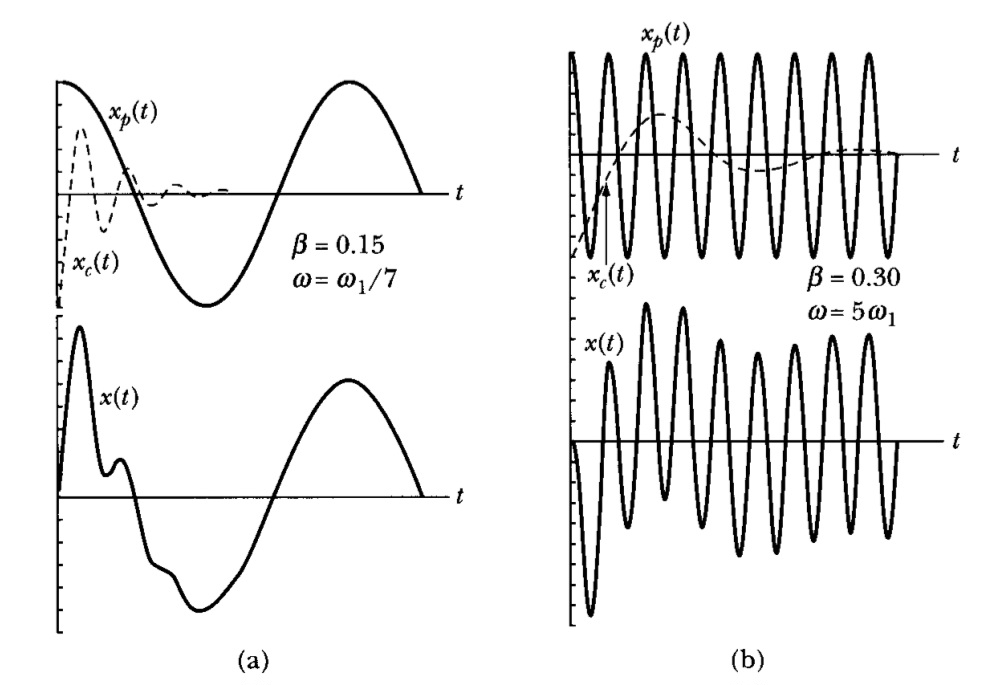
\includegraphics[width=0.7\linewidth]{figure2.6.jpg}
    \caption{사인형 구동력을 받는 강제 조화 진동자의 운동이다. 위쪽 그래프는 과도해 $x_c(t)$와 정상해 $x_p(t)$를, 아래쪽 그래프는 둘의 합인 일반해를 나타낸다. (a)는 구동력의 진동수 $\omega$가 감쇠 조화 진동자의 진동수 $\omega_1$보다 작은 경우, (b)는 그 반대의 경우이다.}
    \label{fig:2.6}
\end{figure}

식 \ref{eq:2.54}의 두 번째 줄은 강제 조화 진동의 위상차 $\delta$를 나타낸다. $\omega_0 \gg \omega$인 경우 $\delta$는 0으로 수렴하여 외부 구동력과 그 응답으로 나타나는 물체의 운동은 거의 비슷한 위상을 가진다. 반면 $\omega_0 \approx \omega$의 경우 $\delta \approx \pi/2$가 되어 물체의 위상은 구동력의 위상과 $-\pi/2$만큼 차이가 난다. 마지막으로 $\omega_0 \ll \omega$인 경우 $\delta$는 $\pi$로 수렴하고, 물체의 위상은 구동력의 위상에 반전된다. 즉, $-\pi$의 위상차를 가진다.   

한편 \textbf{공명(resonance)} 현상은 강제 조화 진동자에서 나타나는 대표적인 물리적 현상이다. 그네를 미는 사람이 어떤 진동수로 힘을 주어야 가장 잘 밀 수 있을까? 이에 답하기 위해 진폭 $D(\omega)$가 최대가 되는 구동력의 진동수 $\omega_R$를 구하면
\begin{equation}
    \omega_R = \sqrt{\omega_0^2-2\beta^2} \label{eq:2.55}
\end{equation}
가 나온다. 이 값을 단순 조화 진동의 진동수 $\omega_0$, 감쇠 조화 진동의 진동수 $\omega_1$과 비교하면 $\omega_0>\omega_1>\omega_R$이다. 흥미롭게도 만약 계의 감쇠 계수 $\beta$가 매우 작아지면 $\omega_R$은 $\omega_0$로 수렴하고, 이때 진폭은 무한대로 발산한다. 즉, 진폭이 커져 계 자체가 파괴된다. 이는 물체의 기본 진동수 $\omega_0$와 아주 유사한 진동수를 가진 구동력이 작용할 때 물체가 급격한 진동을 일으켜 파괴될 수 있다는 사실을 의미하며, 이것의 유명한 예시로는 목소리로 와인잔 깨기 등이 있다.

공명은 비단 진폭만을 대상으로 하는 개념이 아니다. 이번에는 운동 에너지의 공명 진동수를 계산해 보자. 우리는 식 \ref{eq:2.54}의 첫째 줄을 시간에 대해 미분하여
\begin{equation}
    \dot{x}(t) = \frac{-A\omega}{\sqrt{(\omega_0^2-\omega^2)^2+4\beta^2 \omega^2}} \sin{(\omega t-\delta)} \label{eq:2.56}
\end{equation}
를 얻고, 이를 통해 운동 에너지 $T$를
\begin{equation}
    T= \frac{mA^2}{2}\frac{\omega^2}{(\omega_0^2-\omega^2)^2+4\beta^2 \omega^2} \sin^2{(\omega t-\delta)} \label{eq:2.57}
\end{equation}
와 같이 쓸 수 있다. 시간에 독립적인 운동 에너지를 구하기 위해 진동의 한 주기에서의 $T$의 평균값을 구하면
\begin{equation}
    \langle T \rangle = \frac{mA^2}{4}\frac{\omega^2}{(\omega_0^2-\omega^2)^2+4\beta^2 \omega^2} \label{eq:2.58}
\end{equation}
이고\footnote{사인과 코사인 함수의 제곱은 한 주기에서의 평균값이 항상 $1/2$이다.}, 이를 바탕으로 $\langle T \rangle$가 최대가 되는 진동수 $\omega_E$를 구하면
\begin{equation}
    \omega_E=\omega_0 \label{eq:2.59}
\end{equation}
를 얻는다. $\omega_R \neq \omega_E$임에 주의하라. 퍼텐셜 에너지는 진폭의 제곱에 비례하므로, 퍼텐셜 에너지의 공명 진동수는 $\omega_R$이다. 운동 에너지와 퍼텐셜 에너지의 공명 진동수가 다르다는 사실은 강제 조화 진동자의 에너지가 보존되지 않는다는 사실을 나타낸다.

\section{푸리에 급수 (Fourier Series)}
앞선 절에서 우리는 구동력의 형태를 사인형으로 제한했다. 이제 조건을 조금 완화하여 임의의 주기적인 구동력 $F(t)$가 주어지는 경우를 보자. 이때의 운동 방정식은 어떻게 풀어야 할까? 답은 \textbf{푸리에 급수(Fourier series)}를 이용하여 $F(t)$를 사인형 구동력의 합으로 나타내는 것이다.

푸리에 급수를 설명하기 위해선 다음과 같은 세 등식이 필요하다.
\begin{equation}
\begin{split}
     \frac{1}{2\pi}\int_{-\pi}^{\pi} \sin{(mx)}\sin{(nx)} \,\mathrm{d}x &= \frac{1}{2}\delta_{m,n} \\
     \frac{1}{2\pi}\int_{-\pi}^{\pi} \cos{(mx)}\cos{(nx)} \,\mathrm{d}x &= \frac{1}{2}\delta_{m,n} \\
     \frac{1}{2\pi}\int_{-\pi}^{\pi} \sin{(mx)}\cos{(nx)} \,\mathrm{d}x &= 0  
\end{split} 
\label{eq:2.60}
\end{equation}
이때 $\delta_{m,n}$은 크로네커 델타이다. 식 \ref{eq:2.60}의 첫 번째 줄을 증명해 보자. 삼각함수의 합차공식
\begin{equation}
    \sin A \sin B = \frac{1}{2}\big(\cos(A-B) - \cos(A+B)\big) \label{eq:2.61}
\end{equation}
을 적용하면, 좌변은
\begin{equation}
    \frac{1}{2\pi} \int_{-\pi}^{\pi} \sin{(mx)}\sin{(nx)} \,\mathrm{d}x = \frac{1}{4\pi} \int_{-\pi}^{\pi}\cos{[(m-n)x]}-\cos{[(m+n)x]} \,\mathrm{d}x
    \label{eq:2.62}
\end{equation}
로 바뀐다. 피적분함수가 코사인 함수이므로 원시함수는 사인 함수일 것이다. 이때 $m \neq n$이면, 즉 $m-n \neq 0$이면 정수 $k$에 대해 $\sin(k\pi) = 0$이므로 결과가 0이다. 한편 $m=n$이면, 직접 계산하여
\begin{equation}
   \frac{1}{4\pi}\int_{-\pi}^{\pi}1-\cos{(2nx)} \,dx = \frac{1}{4\pi}\left[x-\frac{1}{2n}\sin{(2nx)}\right]_{-\pi}^{\pi} = \frac{1}{2} \label{eq:2.63}
\end{equation}
 을 얻는다. 두 경우를 종합하면 결과는 $\frac{1}{2}\delta_{m,n}$. 식 \ref{eq:2.60}의 두 번째 줄은 삼각함수의 합차공식을 적용하여 비슷한 방식으로 증명 가능하며, 세 번째 줄은 원점을 기준으로 대칭적인 구간에서의 기함수 적분이므로 계산할 것도 없이 0임을 알 수 있다.

이제 $2\pi$의 주기를 가지는 함수 $F(x)$를
\begin{equation}
    F(x) = \sum_{n=0}^{\infty}{a_n\sin{nx}}+\sum_{n=0}^{\infty}{b_n\cos{nx}} \label{eq:2.64}
\end{equation}
와 같이 나타내자.\footnote{이렇게 나타낼 수 있는지, 혹은 이 값이 수렴하는지에 대한 논의는 넘어간다. 제곱적분가능한 임의의 주기 함수는 사인 함수와 코사인 함수의 무한합으로 나타낼 수 있다. 이는 삼각함수계가 해당 공간에서 직교성(orthogonality)과 완비성(completeness)을 가지기 때문이다. 특히 식 \ref{eq:2.60}은 이들의 직교성을 설명한다. 완비성의 증명은 조금 어렵다.} 우리의 목표는 계수 $a_n$과 $b_n$을 결정하는 것이다. $m \neq 0$에 대해 양변에 $\sin{(mx)}$를 곱하고 구간 $[-\pi, \pi]$에 대해 적분하면, 식 \ref{eq:2.60}을 활용하여
\begin{equation}
\begin{split}
    \int_{-\pi}^{\pi} F(x)\sin(mx)\,\mathrm{d}x
    &= \sum_{n=0}^{\infty} a_n
       \int_{-\pi}^{\pi}\sin(nx)\sin(mx)\,\mathrm{d}x \\
    &\quad + \sum_{n=0}^{\infty} b_n
       \int_{-\pi}^{\pi}\cos(nx)\sin(mx)\,\mathrm{d}x \\
    &= \sum_{n=0}^{\infty} a_n \pi \delta_{m,n} = \pi a_m \quad (m \ge 1)
\end{split}
\label{eq:2.65}
\end{equation}
를 얻는다. 이때 $m, n$은 더미 변수이므로 상호 교환하여
\begin{equation}
    a_n = \frac{1}{\pi} \int_{-\pi}^{\pi} F(x)\sin(nx)\,\mathrm{d}x \quad (n \ge 1) \label{eq:2.66}
\end{equation}처럼 쓸 수 있다. 이와 비슷하게 식 \ref{eq:2.64}의 양변에 $\cos{(mx)}$를 곱하고 구간 $[-\pi, \pi]$에 대해 적분하면
\begin{equation}
    b_n = \frac{1}{\pi} \int_{-\pi}^{\pi} F(x)\sin(nx)\,\mathrm{d}x \quad (n \ge 1) \label{eq:2.67}
\end{equation}도 얻을 수 있다.

한편 $\cos{0}=1$, $\sin{0}=0$이므로, 식 \ref{eq:2.64}는
\begin{equation}
    F(x) = \sum_{n=1}^{\infty}{a_n\sin{nx}}+\sum_{n=1}^{\infty}{b_n\cos{nx}}+b_0 \label{eq:2.68}
\end{equation}
로 바꾸어 쓸 수 있다. 양변을 구간 $[-\pi, \pi]$에 대해 적분하면, 삼각함수의 경우 그 결과가 0이므로 간단히
\begin{equation}
    \int_{-\pi}^{\pi}F(x) \,\mathrm{d}x = 2\pi b_0 \label{eq:2.69}
\end{equation}
가 된다. 이를 $b_0$에 대해 정리하면
\begin{equation}
    b_0 = \frac{1}{2\pi} \int_{-\pi}^{\pi}F(x) \,\mathrm{d}x \label{eq:2.70}
\end{equation}
를 얻는다. 이렇게 구한 $a_n, b_n, b_0$는 \textbf{푸리에 계수(Fourier coefficients)}이다.

지금까지의 논의는 주기가 $2\pi$인 함수 $F(x)$에 대해 이루어졌다. 주기가 $T$인 함수 $F(t)$에 대해선, 식 \ref{eq:2.60}의 변수를 $\omega = 2\pi / T, x=\omega t$로 바꾸어
\begin{equation}
\begin{aligned}
    F(t) &= b_{0} + \sum_{n=1}^{\infty} a_{n}\sin(n\omega t) + \sum_{n=1}^{\infty} b_{n}\cos(n\omega t) \\
    a_{n} &= \frac{2}{T} \int_{-T/2}^{T/2} F(t)\sin(n\omega t)\,\mathrm{d}t \quad (n \ge 1) \\
    b_{n} &= \frac{2}{T} \int_{-T/2}^{T/2} F(t)\cos(n\omega t)\,\mathrm{d}t \quad (n \ge 1) \\ 
    b_{0} &= \frac{1}{T} \int_{-T/2}^{T/2} F(t)\,\mathrm{d}t \label{eq:2.71}
\end{aligned}
\end{equation}
로 나타내면 된다. 모든 주기함수를 이렇게 표현할 수 있다니, 놀랍지 않은가? 마법은 여기서 끝나지 않는다. 식 \ref{eq:2.71}은 한 주기에 대한 적분이므로, 적분 구간을 임의의 한 주기 구간 $[t_0, t_0 + T]$로 두어도 그 결과가 동일하다. 이것은 때에 따라 엄청난 이점이 된다. 계산에 편리한 $t_0$를 마음대로 설정할 수 있기 때문이다.

이제 결론을 내려 보자. 우리가 궁금해하는 사항은 운동 방정식
\begin{equation}
    \ddot{x} + 2\beta \dot{x} + \omega_0^2 x = \sum_{n=0}^{\infty}\frac{a_n}{m}\sin{(n\omega t)} + \sum_{n=0}^{\infty}\frac{b_n}{m}\cos{(n \omega t)}
\end{equation} \label{eq:T driv}
의 일반해이다. 미분의 선형성을 고려하면, 일반해는
\begin{equation}
    x(t) = x_c(t) + \sum_{n=0}^{\infty}X_n(t) + \sum_{n=0}^{\infty}Y_n(t) \label{eq:2.73}
\end{equation}
의 형태로 주어질 것이 자명하다. 이때 $X_n$과 $Y_n$은 각각 사인 함수와 코사인 함수의 특수해이다. 그런데 식 \ref{eq:2.54}의 결과를 고려하면
\begin{equation}
    \begin{aligned}
        X_n(t) &= \frac{a_n}{m}\frac{1}{\sqrt{(\omega_0^2-n^2\omega^2)^2+4\beta^2 n^2 \omega^2}} \cos{(\omega t-\delta_{X_n})} \\ \delta_{X_n} &= \arctan{\left(\frac{2n\omega \beta}{\omega_0^2-n^2\omega^2}\right)} \\
        Y_n(t) &= \frac{b_n}{m}\frac{1}{\sqrt{(\omega_0^2-n^2\omega^2)^2+4\beta^2 n^2 \omega^2}} \cos{(\omega t-\delta_{Y_n})} \\ \delta_{Y_n} &= \arctan{\left(\frac{2n\omega \beta}{\omega_0^2-n^2\omega^2}\right)}
        \label{eq:2.74}
    \end{aligned}
\end{equation}
이므로, 우리는 이들을 식 \ref{eq:2.73}에 대입하여 일반해를 구할 수 있다.
\begin{examplebox}{예제 2.2}
\begin{example}
주기가 $\tau$이고 진폭이 $A/2$인 톱니파가 구동력으로 주어지는 강제 조화 진동자가 있다. 진동자의 운동 방정식을 풀어라.
\end{example}
\end{examplebox}

\begin{solution}
    톱니파의 식은 다음과 같다.
    \begin{equation}
        F(t) = \frac{A}{\tau}t = \frac{\omega A}{2\pi}t \quad \left(-\frac{\tau}{2} \leq t \leq \frac{\tau}{2}\right)
    \end{equation}
    이를 푸리에 급수로 나타내자. $F(t)$는 기함수이므로 푸리에 계수 중 $b_n$은 0이다. 한편 $a_n$은 식 \ref{eq:2.71}에 따라
    \begin{equation}
        a_{n} = \frac{\omega A}{2\pi}\int_{-\tau/2}^{\tau/2}\sin(n\omega t)\,\mathrm{d}t
    \end{equation} \label{eq:2.76} 로 계산할 수 있고, 이를 풀면
    \begin{equation}
        a_n = \frac{\omega A}{2\pi} \left[-\frac{t\cos{(n\omega t)}}{n\omega} + \frac{\sin{(n\omega t)}}{n^2 \omega^2}
    \right]_{-\tau/2}^{\tau/2} = -\frac{A}{n\pi}\cos{(n\pi)} = \frac{A}{n\pi}{(-1)}^{n+1}
    \end{equation}을 얻는다. 이상의 결과에 따라 톱니파의 푸리에 급수는
    \begin{equation}
        F(t) = \sum_{n=0}^{\infty} \frac{A}{n\pi} {(-1)}^{n+1}\sin{(n\omega t)} = \frac{A}{\pi}\left[\sin{\omega t}-\frac{1}{2}\sin{2\omega t}+ \frac{1}{3}\sin{3\omega t}- \cdots \right]
        \label{eq:2.78}
    \end{equation}와 같다. 이들의 모습은 그림 \ref{fig:2.7}과 그림 \ref{fig:2.8}을 참고하라.
\begin{figure}
    \centering
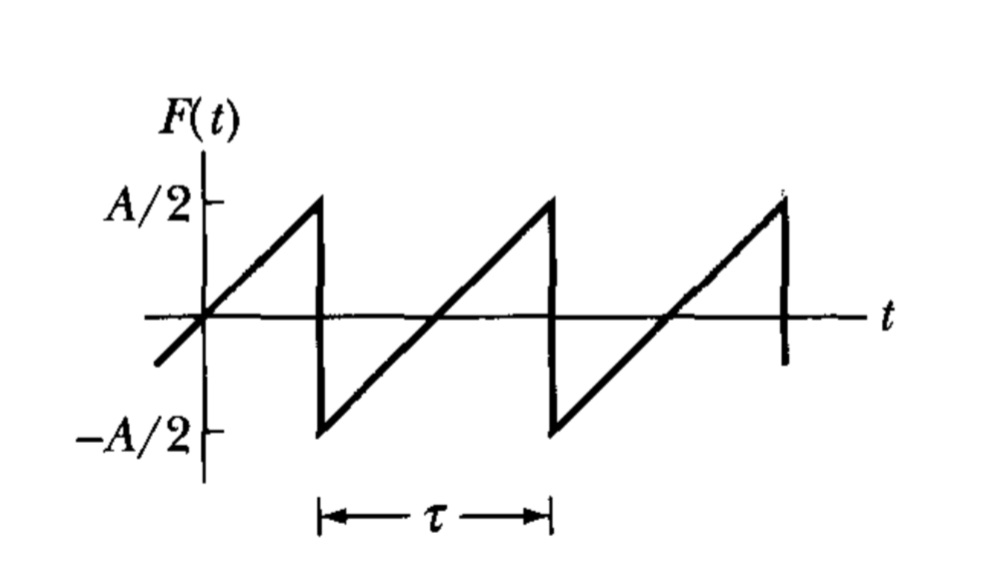
\includegraphics[width=0.5\linewidth]{figure2.7.jpg}
    \caption{예제 2.2의 톱니파이다.}
    \label{fig:2.7}
\end{figure}

\begin{figure}
    \centering
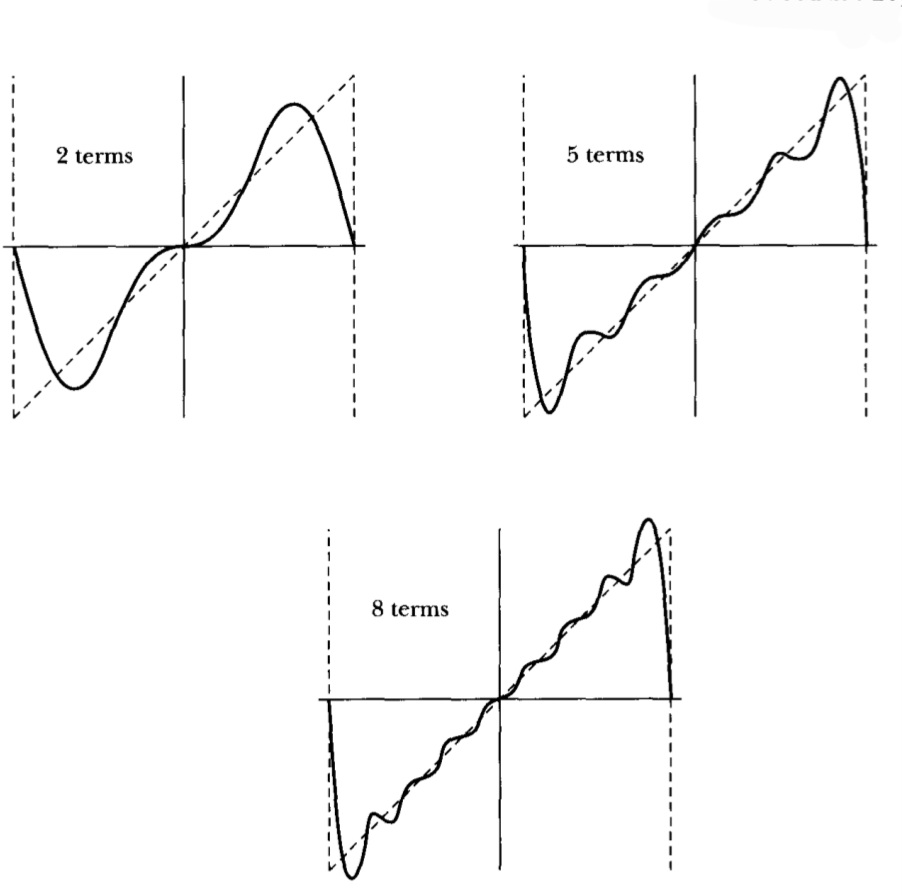
\includegraphics[width=0.7\linewidth]{figure2.8.jpg}
    \caption{예제 2.2의 톱니파를 푸리에 급수로 전개하였다.}
    \label{fig:2.8}
\end{figure}


이제 운동 방정식을 풀자. 우리는 식 \ref{eq:2.74}를 적용하여 특수해 $x_p(t)$를 
    \begin{equation}
    \begin{aligned}
        x_p(t) &= \sum_{n=0}^{\infty}\frac{{(-1)}^{n+1}A}{nm\pi \sqrt{(\omega_0^2-n^2\omega^2)^2+4\beta^2 n^2 \omega^2}} \cos{(\omega t-\delta)} \\
        \delta &= \arctan{\left(\frac{2n\omega \beta}{\omega_0^2-n^2\omega^2}\right)}
    \end{aligned}
    \end{equation}와 같이 쓸 수 있다. 일반해를 얻으려면 여기에 식 \ref{eq:2.46}에서 얻은 보조해 $x_c(t)$를 더하면 된다. 초기 조건 2개가 주어진다면 $x_c(t)$는 완벽히 풀릴 것이다.
\end{solution}

\noindent\rule{\textwidth}{0.8pt} % 본문 전체 너비만큼 0.8pt 두께의 검은 줄을 긋습니다.
\vspace{1em} % 줄 아래에 약간의 여백을 줍니다.

주기함수를 푸리에 급수로 전개할 때 알아두어야 할 사실이 있다. 이론적으로 우리는 사인형 함수의 무한합을 통해 어떤 함수든지 푸리에 급수로 근사할 수 있다. 그러나 현실에선 사인파를 무한히 더할 수 없기 때문에, 적당히 많은 양의 신호를 중첩시켜 주기함수를 구현한다. 이때 주기함수의 불연속점 부근에서는 신호가 튀는(overshoot) 현상이 발생하는데, 이를 \textbf{깁스 현상(Gibbs phenomenon)}이라고 한다. 깁스 현상에 의해 발생하는 overshoot의 간극은 원래 값 대비 약 8.9490...\% 정도 크다.\footnote{정확히는 $Si(\pi)/\pi - 1/2$만큼 더 크다. 이때 $Si(x)$는 사인 적분 함수이다.}

\section{강제 조화 진동 (Driven Harmonic Oscillations)}
이제 우리는 이 장에서 단 하나만의 과제를 남겨 두고 있다. 구동력 $F(t)$가 주기함수가 아니라면, 운동 방정식
\begin{equation}
    \ddot{x} + 2\beta \dot{x} + \omega_0^2x = \frac{F(t)}{m} \label{eq:2.80}
\end{equation}
을 어떻게 풀어야 하는가?

미분방정식을 배운 독자들이라면, \textbf{라플라스 변환(Laplace transform)}을 통해 선형 미분방정식을 쉽게 풀 수 있다는 사실을 알 것이다. 정확히 똑같은 방식이 이곳에도 적용된다. 따라서 이 절을 완벽히 이해하려면 라플라스 변환을 알고 있어야 한다. 하지만 복잡한 내용을 언급하기 전에, 가장 간단한 구동력의 형태부터 출발하자. 다음과 같은 함수
\begin{equation}
    \frac{F(t)}{m} = H(t) = \begin{cases}
    0 & (t<0) \\
    a & (t \ge 0) \end{cases}
    \label{heaviside step function}
\end{equation}
처럼 말이다. 이 함수는 \textbf{헤비사이드 계단함수(Heaviside step function)}로 알려져 있다. 이때 $t \ge 0$에서 운동 방정식은 다음과 같다.
\begin{equation}
    \ddot{x} + 2\beta \dot{x} + \omega_0^2x = a \label{eq:2.82}
\end{equation}
초기 조건을 $x(0)=0$, $\dot{x}(0)=0$으로 가정하자. 앞서 언급했듯, 식 \ref{eq:2.82}의 일반해 $x_H(t)$는 특수해 $x_p(t)$와 보조해 $x_c(t)$의 합이다. 그런데 우변이 상수이므로 특수해는 간단히 $x_p(t) = a/\omega_0^2$가 된다. 따라서 일반해는
\begin{equation}
    x_H(t) = e^{-\beta t}[A_1e^{i\omega_1t}+A_2e^{-i\omega_1t}] + \frac{a}{\omega_0^2} \label{eq:2.83}
\end{equation}
라고 쓸 수 있다. 여기서 $\omega_1 \equiv \sqrt{\omega_0^2-\beta^2}$의 치환을 적용하였다.

초기 조건 2개가 주어졌으므로 우리는 미지수 $A_1, A_2$의 값을 모두 결정할 수 있다. $x(0)=0$, $\dot{x}(0)=0$을 대입하여 풀면
\begin{equation}
    \begin{aligned}
        A_1 &= -\frac{a}{2\omega_0^2} \left(1-\frac{i\beta}{\omega_1} \right) \\
        A_2 &= -\frac{a}{2\omega_0^2} \left(1+\frac{i\beta}{\omega_1} \right) \\
    \end{aligned}
    \label{eq:2.84}
\end{equation}를 얻고, 이를 활용하면 일반해는
\begin{equation}
    \begin{split}
        x_H(t) &= e^{-\beta t}\left[-\frac{a}{2\omega_0^2} \left(1-\frac{i\beta}{\omega_1} \right)e^{i\omega_1t}-\frac{a}{2\omega_0^2} \left(1+\frac{i\beta}{\omega_1} \right)e^{-i\omega_1t}\right] + \frac{a}{\omega_0^2} \\
        &= e^{-\beta t}\left[-\frac{a}{2\omega_0^2}(e^{i\omega_1t}+e^{-i\omega_1t})+\frac{ia\beta}{2\omega_0^2 \omega_1}(e^{i\omega_1t}-e^{-i\omega_1t})\right] + \frac{a}{\omega_0^2} \\
        &= e^{-\beta t}\left[-\frac{a}{\omega_0^2}\cos{(\omega_1t)}-\frac{a\beta}{\omega_0^2 \omega_1}\sin{(\omega_1t)}\right] + \frac{a}{\omega_0^2} \\
        &= \frac{a}{\omega_0^2}\left[1-e^{-\beta t}\cos{(\omega_1t)}-\frac{\beta e^{-\beta t}}{\omega_1}\sin{(\omega_1t)}\right] \label{eq:2.85}
    \end{split}
\end{equation}
가 된다.

다음으로 알아볼 것은 $F(t)$가 \textbf{임펄스 함수(impulse function)}인 경우이다. 임펄스 함수는
\begin{equation}
    \frac{F(t)}{m} = I(t) = \begin{cases}
    0 & (t<0) \\
    a & (0 \le t \le \tau) \\
    0 & (t > \tau) \end{cases}
    \label{eq:2.86}
\end{equation}
와 같고, 헤비사이드 계단함수를 통해
\begin{equation}
    I(t) = H(t)-H(t-\tau) \label{eq:2.87}
\end{equation}
처럼 나타낼 수 있다. 이를 통해 만들어지는 미분방정식의 일반해 $x_I(t)$는 중첩의 원리에 따라 $x_H(t)-x_H(t-\tau)$와 같을 것이다. 이제 우리는 $\tau \to 0$의 극한을 취할 텐데, 이 과정에서 $a \to \infty$로 보내어 $a\tau$를 상수로 만들려고 한다. 직사각형의 너비 $\tau$는 줄이고 높이 $a$는 늘려서 넓이 $a\tau$를 유지한다고 이해하면 좋다. 그러면
\begin{equation}
    \frac{I(t)}{a\tau} = \lim_{\tau \to 0} \frac{1}{a}\frac{H(t)-H(t-\tau)}{\tau} = \frac{1}{a}\frac{dH}{dt} \label{eq:2.88}
\end{equation}가 성립한다. 이때 우리가 정의한 $H(t)$는 $t>0$에서 $a$의 값을 가지므로, 이를 시간에 대해 미분하면 $a\delta(t)$가 된다. 여기서 $\delta(t)$는 \textbf{디랙 델타 함수(Dirac delta function)}로, $t=0$에서 무한대의 값을 가지고 그 외의 구간에서는 0이며 전체 적분 면적은 1인 함수이다. 디렉 델타 함수를 도입하여 식 \ref{eq:2.88}을 다시 쓰면 다음과 같다.
\begin{equation}
    I(t) = a\tau \delta(t) \label{eq:2.89}
\end{equation}

이제 이 구동력에 대한 미분방정식의 해 $x_I(t)$를 구해 보자. 똑같은 극한을 적용하면
\begin{equation}
    x_I(t) = \lim_{\tau \to 0}[x_H(t)-x_H(t-\tau)]
\end{equation}이고, 우변을 $\tau$로 나눈 뒤 곱하면
\begin{equation}
    x_I(t) = \lim_{\tau \to 0}\left[\frac{x_H(t)-x_H(t-\tau)}{\tau}\right] \tau = \tau \frac{d}{dt}x_H(t) \label{eq:2.91}
\end{equation}이다. 식 \ref{eq:2.85}에서 구한 $x_H(t)$를 미분하여 대입하면
\begin{equation}
\begin{aligned}
    x_I(t) &= \tau \frac{d}{dt}x_H(t) \\
    &= \frac{a\tau}{\omega_0^2} \left[ \beta e^{-\beta t} \left( \cos(\omega_1 t) + \frac{\beta}{\omega_1} \sin(\omega_1 t) \right) - e^{-\beta t} \left( -\omega_1 \sin(\omega_1 t) + \beta \cos(\omega_1 t) \right) \right] \\
    &= \frac{a\tau}{\omega_0^2} e^{-\beta t} \left( \frac{\beta^2}{\omega_1} + \omega_1 \right) \sin(\omega_1 t) \\
    &= \frac{a\tau}{\omega_0^2} e^{-\beta t} \left( \frac{\beta^2 + \omega_1^2}{\omega_1} \right) \sin(\omega_1 t) \\
    &= \frac{a\tau}{\omega_1} e^{-\beta t} \sin(\omega_1 t)
\end{aligned} \label{eq:2.92}
\end{equation}를 얻을 수 있다.

마지막 단계는 F(t)가 임의의 함수인 경우이다. 우리는 $F(t)$의 형태가 어떻든지 이를 임펄스 함수의 합으로 표현할 수 있다. 그림 \ref{fig:2.9}를 참고하라. 그렇다면 운동 방정식은 다음과 같다.
\begin{equation}
    \ddot{x} + 2\beta \dot{x}+\omega_0^2x=\sum_{n=-\infty}^{\infty} \frac{F_n(t)}{m}=\sum_{n=-\infty}^{\infty}I_n(t) \label{eq:2.93}
\end{equation}
이때 $n$번째 임펄스 함수 $I_n(t)$는 다음과 같이 정의된다.
\begin{equation}
    I_n(t) = \begin{cases}
        a_n(t_n) &(t_n \le t \le t_{n+1}) \\
        0 & \mathrm{otherwise}
    \end{cases} \label{eq:2.94}
\end{equation}
$I_n(t)$가 계에 작용하는 시간 간격 $t_{n+1}-t_n$을 $\tau$라고 하자. 즉, $\tau$는 그림 속 사각형들의 너비이다. 만약 $\tau$가 매우 작다면 $I_n(t)$에 대한 해 $x_n(t)$는 식 \ref{eq:2.92}에 따라
\begin{equation}
    x_n(t) = \frac{a_n(t_n)\tau}{\omega_1} e^{-\beta (t-t_n)} \sin(\omega_1 (t-t_n)) \label{eq:2.95}
\end{equation}의 형태를 가질 것이다. 그렇다면 $N$번째 임펄스 함수까지의 모든 임펄스 함수에 대한 해 $x(t)$는
\begin{equation}
    x(t) = \sum_{n=-\infty}^{N} \frac{a_n(t_n)\tau}{\omega_1} e^{-\beta (t-t_n)} \sin(\omega_1 (t-t_n)) \quad (t_N < t < t_{N+1}) \label{eq:2.96}
\end{equation}
와 같다. $\tau$를 $\mathrm{d}t$로, $t_n$을 $t'$으로 바꾸고 시그마를 적분으로 교체하면 최종적으로
\begin{equation}
    x(t) = \int_{-\infty}^{t} \frac{a(t')}{\omega_1} e^{-\beta (t-t')} \sin(\omega_1 (t-t'))\, \mathrm{d}t \label{eq:2.97}
\end{equation}
를 얻는다. 이것이 우리가 원하던 일반해이다.

\begin{figure}
    \centering
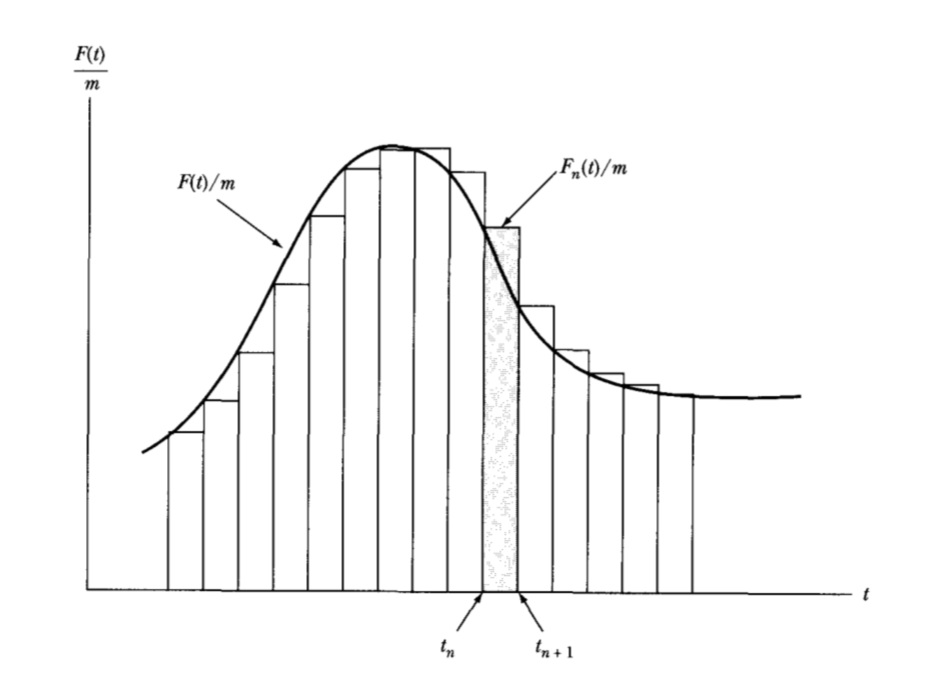
\includegraphics[width=0.7\linewidth]{figure2.9.jpg}
    \caption{임의의 함수 $F(t)$는 임펄스 함수의 합으로 표현할 수 있다.}
    \label{fig:2.9}
\end{figure}

한편 식 \ref{eq:2.97}에 포함된 $a(t')$는 가속도를 의미한다. 따라서 뉴턴의 제2법칙을 적용하면 이 식은
\begin{equation}
    x(t) = \int_{-\infty}^{t} F(t')\frac{1}{m\omega_1} e^{-\beta (t-t')} \sin(\omega_1 (t-t'))\, \mathrm{d}t \label{eq:2.98}
\end{equation}
처럼 바뀐다. 적분 기호 내부에서 외력 $F(t')$에 곱해지는 항은 시각 $t'$에 가해진 단위 충격량에 대해 시각 t에서 계가 보이는 응답을 나타내며, 이 항에는 \textbf{그린 함수(Green's function)}라는 이름이 있다. 충격이 가해지기 전$(t < t')$에는 물리적으로 반응이 일어날 수 없다는 인과 관계를 고려하면, 그린 함수 $G(t, t')$의 정의는
\begin{equation}
    G(t, t') \equiv \begin{cases} \dfrac{1}{m\omega_1} e^{-\beta(t-t')} \sin{(\omega_1 (t-t'))}, & (t \ge t') \\ 0, & (t < t') \end{cases} \label{eq:2.99}
\end{equation}이고, 이를 식 \ref{eq:2.98}에 대입하면
\begin{equation}
    x(t) = \int_{-\infty}^{t} F(t') G(t, t') \, \mathrm{d}t'
    \label{eq:2.100}
\end{equation}
을 얻는다. 이 식은 임의의 외력 $F(t)$에 대한 계의 반응 $x(t)$가 그린 함수와의 컨볼루션(convolution) 적분으로 나타난다는 사실을 보여준다. 덧붙이자면, $t < t'$에서 그린 함수의 값이 0이기 때문에 우리는 식 \ref{eq:2.100}의 적분 구간을 $[-\infty, \infty]$로 바꾸어 써도 무방하다.

지금까지의 과정을 정리해 보자. 우리가 이 절에서 풀고 싶었던 것은 임의의 복잡한 힘 $F(t)$가 주어졌을 때의 운동 방정식이다. 다행히 미분방정식이 선형이므로 우리는 강력한 마법을 쓸 수 있었다. 바로 각각의 힘에 대한 결과를 따로 구한 후 마지막에 다 더해도 된다는 것. 그래서 우리는 구동력 $F(t)$를 시간 $t'$에 가해지는 충격량 $I(t)$의 연속으로 생각했고, 이를 바탕으로 식 \ref{eq:2.100}과 같은 해를 구했다. 그린 함수의 형태를 보면 이는 물리적으로 아주 자연스러운 결과다. $(t \ge t')$라는 구간은 타격을 받고 난 후에야 물체가 반응한다는 인과 관계를, $\sin{(\omega_1 (t-t'))}$ 항은 초기 조건 $x(0)=0$, $\dot{x}(0)=0$을 고려한 물체의 진동을, $e^{-\beta(t-t')}$ 항은 감쇠력에 의한 진폭의 감소를 나타내기 때문이다.

마지막으로 소개할 내용은 라플라스 변환을 통한 운동 방정식의 풀이이다. 임펄스 함수가 구동력으로 주어진 경우를 보자. 운동 방정식은, 식 \ref{eq:2.89}에 따라
\begin{equation}
    \ddot{x} + 2\beta \dot{x}+\omega_0^2x = a \tau \delta(t) \label{eq:2.101}
\end{equation}
이다. 역시 초기 조건 $x(0) = 0$, $\dot{x}(0) = 0$을 가정하자. 양변에 라플라스 변환 $\mathcal{L}{f(t)} = X(s)$를 취하면, $\mathcal{L}\{\ddot{x}\} = s^2 X(s)$, $\mathcal{L}{\dot{x}} = s X(s)$가 되고 디랙 델타 함수의 라플라스 변환은 $\mathcal{L}\{\delta(t)\} = 1$이므로 다음이 성립한다.
\begin{equation}
    s^2 X(s) + 2\beta s X(s) + \omega_0^2 X(s) = a\tau
\end{equation}
이를 $X(s)$에 대해 묶어서 정리하면
\begin{equation}
    X(s) = \frac{a\tau}{s^2 + 2\beta s + \omega_0^2} \label{eq:2.103}
\end{equation}
이다. 이제 역라플라스 변환을 수행하기 위해 분모를 완전제곱식 형태로 변형하자. 즉, $s^2 + 2\beta s + \omega_0^2 = (s + \beta)^2 + (\omega_0^2 - \beta^2)$의 형태로 나타내자. underdamping인 상황을 가정하면, $\omega_1^2 = \omega_0^2 - \beta^2$이므로 식은 다음과 같이 변형된다.
\begin{equation}
    X(s) = \frac{a\tau}{(s + \beta)^2 + \omega_1^2}
\end{equation}
이 식을 라플라스 역변환 공식 $\mathcal{L}^{-1}\left\{ \frac{\omega}{(s + b)^2 + \omega^2} \right\} = e^{-bt} \sin(\omega t)$의 형태에 맞추기 위해 분모와 분자에 $\omega_1$을 곱하면
\begin{equation}
    X(s) = \frac{a\tau}{\omega_1} \frac{\omega_1}{(s + \beta)^2 + \omega_1^2}
\end{equation}
처럼 바뀐다. 양변에 역라플라스 변환을 취해 $x_I(t)$를 구하면 결과는 다음과 같다.
\begin{equation}
    x_I(t) = \frac{a\tau}{\omega_1} e^{-\beta t} \sin(\omega_1 t)
\end{equation}
이 결과는 앞서 계단 함수 응답의 중첩과 극한을 이용해 유도한 결과와 완벽히 일치한다. 라플라스 변환을 이용하면 복잡한 계산 없이도 미분방정식을 풀어낼 수 있으며, 특히 임의의 구동력 $F(t)$가 주어진 경우라면 그린 함수 $G(t, t')$을 빠르게 구할 수 있다.


\newpage
% Chapter 3 시작
\chapter{비선형 진동과 카오스 (Nonlinear Oscillations and Chaos)}

\section{개요}
2장에 등장한 진동자의 운동 방정식은 모두 선형 미분방정식이다. 그러나 실제 자연 현상은 대부분 비선형 미분방정식으로 기술된다. 즉, 1차원 상에서 움직이는 물체의 운동 방정식
\begin{equation}
    m\ddot{x}+f(\dot{x})+g(x)=h(t)
\end{equation}
에서 $f(\dot{x})$나 $g(x)$가 선형보다 높은 차수의 항을 포함하거나 초월함수의 형태를 띠는 경우이다. 비선형 미분방정식은 해석적으로 완전한 해를 항상 구할 수 없기 때문에 위상도를 분석하거나 수치해석적 방법을 쓰는 등 특별한 접근법이 필요하다.

한편 19세기 초 프랑스의 수학자 라플라스는 우주에 있는 모든 입자의 위치와 속도, 그리고 그들을 지배하는 물리 법칙들을 안다면 미래의 모든 현상을 완벽히 기술할 수 있다는 결정론적(deterministic) 세계관을 주창했다.\footnote{이것이 바로 라플라스의 악마(Laplace's demon)이다.} 하지만 현대 과학에 따르면 이는 불가능하다. 자연의 많은 계는 \textbf{카오스(chaos)}를 보이기 때문이다. 여기서 카오스란 계가 물리 법칙에 따라 철저히 결정론적으로 전개됨에도 불구하고 발생하는 결정론적 카오스(deterministic chaos)를 의미한다. 카오스의 핵심은 계가 초기 조건에 극도로 민감하게 의존한다는 데 있으며, 우리는 물체의 운동을 완벽히 예측할 수 있을 정도로 초기 조건을 측정할 능력이 없다.

카오스는 비선형계에서만 발생한다. 주목해야 할 점은 비선형성이 카오스가 발생하기 위한 필요조건이긴 하지만 충분조건은 아니라는 것이다. 계가 언제 카오스 현상을 보일지 예측하는 일반적인 방법론은 존재하지 않는다. 따라서 우리는 이 장에서 몇 가지 비선형 미분방정식을 풀고, 어떤 비선형계에서 카오스 현상이 발생하는지 알아볼 것이다.

\section{비선형 진동 (Nonlinear Oscillations)}
우리는 2장에서 아주 작은 변위 $x$를 가정하여 복원력을 $-kx$로 근사했다. 그러나 $x$의 크기가 무시할 수 없을 정도로 크다면 이야기가 달라진다. 복원력의 고차항까지 고려해야 하기 때문이다.

일반적으로 자연에 나타나는 비선형계는 평형점에 대칭이다. 즉, 평형점으로부터 $x$만큼 떨어지든 $-x$만큼 떨어지든 물체는 같은 크기의 복원력을 받는다. 방향만 반대일 뿐이다. 만약 $x=0$을 평형점으로 간주한다면, 이러한 복원력은 기함수가 된다. 이제 선형이 아닌 가장 간단한 기함수를 복원력으로 고려하면
\begin{equation}
    F(x) = -kx + \epsilon x^3
\end{equation}
이고, 퍼텐셜은
\begin{equation}
    U(x) = \frac{1}{2}kx^2 - \frac{1}{4}\epsilon x^4
\end{equation}
이다. 퍼텐셜 함수는 자연스럽게 우함수가 된다.

퍼텐셜 함수의 개형은 $\epsilon$의 부호에 따라 조금씩 달라진다. 구체적으로, $\epsilon>0$이면 변위 $\vert{}x\vert{}$가 증가할 때 복원력의 크기가 선형 근사값보다 약해지며 퍼텐셜 우물이 평평해진다. 우리는 이 경우를 soft system이라고 한다. 반면 $\epsilon<0$인 경우 변위 $\vert{}x\vert{}$가 증가할 때 복원력의 크기는 선형 근사값보다 강해지며 퍼텐셜 우물은 가파라진다. 우리는 이 경우를 hard system이라고 한다. Soft system과 hard system의 구분은 비선형계의 운동을 직관적으로 이해하는 데 큰 도움이 된다.

물론 평형점에 대칭이 아닌 비선형계도 존재할 수 있다. 이 경우 가장 간단한 복원력의 형태는 $F=-kx+\lambda x^2$이며, 계는 $\lambda >0$일 때 soft system, $\lambda<0$일 때 hard system이 될 것이다.

\section{평면 진자 (Plane Pendulum)}
비선형계의 가장 유명한 예시는 단진자와 같은 평면 진자이다. 우리는 예제 2.1에서 단진자와 관련된 문제를 풀었지만, 이는 각 $\theta$가 매우 작다고 가정하여 $\sin{\theta} \approx \theta$로 근사한 경우였다. 단진자의 정확한 운동 방정식은 다음과 같다.
\begin{equation}
    \ddot{\theta}+\frac{g}{l}\sin{\theta} = 0
    \label{eq:3.4}
\end{equation}
이는 명백히 비선형 미분방정식이다. 식 \ref{eq:3.4}를 어떻게 풀어야 할까? 우리는 미분방정식을 직접 푸는 대신 에너지 보존 법칙을 통해 우회하고자 한다.

진자의 퍼텐셜 에너지가 최하점($\theta = 0$)에서 $0$이 된다고 가정하자. 이때 운동 에너지와 퍼텐셜 에너지는 다음과 같다.
\begin{equation}
    \begin{aligned}
        T &= \frac{1}{2}I\omega^2 = \frac{1}{2}ml^2\dot{\theta}^2 \\
        U &= mgl(1-\cos{\theta})
    \end{aligned}
\end{equation}
이제 $\theta = \theta_0$를 진자의 최고점으로 두면
\begin{equation}
    \begin{aligned}
        T(\theta=\theta_0) &= 0 \\
        U(\theta=\theta_0) &= E = mgl(1-\cos{\theta_0})
    \end{aligned}
\end{equation}
이다. 삼각함수의 반각공식 $\cos{\theta}=1-2\sin^2{(\theta / 2})$을 활용하면, 에너지는
\begin{equation}
    \begin{aligned}
        E &= 2mgl \sin^2{(\theta_0/ 2)}\\
        U &= 2mgl \sin^2{(\theta / 2)} \\
        T &= E-U = 2mgl [\sin^2{(\theta_0/2)} - \sin^2{(\theta / 2)}]
    \end{aligned}
    \label{eq:3.7}
\end{equation}
로 쓸 수 있다. 이상의 결과에서
\begin{equation}
    \begin{aligned}
        \frac{1}{2}ml^2\dot{\theta}^2 &= 2mgl [\sin^2{(\theta_0/2)} - \sin^2{(\theta / 2)}] \\
        \dot{\theta} &= 2 \sqrt{\frac{g}{l}}[\sin^2{(\theta_0/2)} - \sin^2{(\theta / 2)}]^{1/2}
    \end{aligned}
    \label{eq:3.8}
\end{equation}
를 얻는다. 편의를 위해 각도가 증가하는 경우만 생각했다.

먼저 단진자의 주기 $\tau$를 구해 보자. 식 \ref{eq:3.8}을 변형하면
\begin{equation}
    \mathrm{d}t = \frac{1}{2}\sqrt{\frac{l}{g}}[\sin^2{(\theta_0/2)} - \sin^2{(\theta / 2)}]^{-1/2} \mathrm{d}\theta
    \label{eq:3.9}
\end{equation}이므로, 적분하면 시간 $t(\theta)$를 구할 수 있다. 그런데 진자가 $\theta=0$부터 $\theta=\theta_0$까지 운동하는 데 걸린 시간은 전체 주기 $\tau$의 $1/4$배이므로
\begin{equation}
    \tau = 2\sqrt{\frac{l}{g}} \int_{0}^{\theta_0}[\sin^2{(\theta_0/2)} - \sin^2{(\theta / 2)}]^{-1/2} \mathrm{d}\theta
    \label{eq:3.10}
\end{equation}
가 성립한다. 이제 남은 건 이 적분을 어떻게 풀 수 있을까에 대한 문제이다. 놀랍게도 변수 치환
\begin{equation*}
\begin{aligned}
    z &\equiv \frac{\sin{(\theta/2)}}{\sin{(\theta_0/2})}, \quad k \equiv \sin{(\theta_0/2}) \\
    \mathrm{d}z &= \frac{\cos{(\theta/2)}}{2\sin{(\theta_0/2})}\mathrm{d}\theta = \frac{\sqrt{1-k^2z^2}}{2k}\mathrm{d}\theta
\end{aligned}
\end{equation*}
을 적용하면 식 \ref{eq:3.10}은
\begin{equation}
    \tau = 4\sqrt{\frac{l}{g}} \int_0^1 \frac{1}{\sqrt{1-z^2}\sqrt{1-k^2z^2}}\mathrm{d}z
\end{equation}
처럼 바뀌고, 이 적분은 \textbf{제1종 완전 타원 적분(complete elliptic integral for the first kind)} $K(k)$의 형태이므로 주기는 다음과 같다.
\begin{equation}
    \tau = 4\sqrt{\frac{l}{g}}K(k)
\end{equation}
한편 $K(k)$는 급수 형태로
\begin{equation}
    \begin{aligned} K(k) &=\frac{\pi}{2} \left[1+ \sum_{n=1}^{\infty }\left [ \frac{(2n-1)!!}{(2n)!!} \right ]^{2}{k^{2n}} \right]\\& =\frac{\pi}{2} \sum_{n=0}^{\infty }\left [ \frac{(2n)!}{2^{2n}\left(n!\right)^{2}} \right ]^{2}k^{2n} \\
    &= \frac{\pi}{2}\left[1+ \left(\frac{1}{2}\right)^2 k^2 + \left( \frac{1 \cdot 3}{2 \cdot 4} \right)^2 k^4 + \dots \right]
    \end{aligned}
    \label{eq:3.13}
\end{equation}
와 같이 전개할 수 있다. 이를 바탕으로 주기를 다시 쓰면
\begin{equation}
    \tau = 2\pi \sqrt{\frac{l}{g}} \left[1+ \frac{1}{4} k^2 + \frac{9}{64} k^4 + \dots \right]
\end{equation}
이다. 만약 $k$의 크기가 크다면, 주기를 정확히 구하기 위해선 더 높은 차수의 항까지 고려해야 할 필요가 있다. 하지만 $k=\sin{(\theta_0 / 2)}$가 충분히 작다면, 테일러 전개를 통해 $\sin{(\theta_0/2)} \approx (\theta_0/2) - (\theta_0^3/48)$로 근사할 수 있으므로
\begin{equation}
    \tau = 2\pi \sqrt{\frac{l}{g}} \left[1+\frac{1}{16}\theta_0^2 + \frac{11}{3072}\theta_0^4 \right]
    \label{eq:3.15}
\end{equation}
을 얻는다. 이 식은 수렴 속도가 상당히 빠르므로, 우리는 작은 각 $\theta_0$에 대해 단진자의 주기를 식 \ref{eq:2.14}처럼 쓸 수 있다. 구체적인 오차율은 표 \ref{table:3.1}을 참고하라. 식 \ref{eq:3.13}의 수렴 구간은 $0 < k < 1$이므로 단진자는 구간 $0 < k < 1$에서 진동하며, $k \geq 1$이면 주기가 무한대로 발산한다.

\begin{table}[htbp]
\centering
\caption{초기 각도 $\theta_0$에 따른 실제 주기의 오차율}
\label{tab:pendulum_period}
\vspace{0.5em} % 캡션과 표 상단 선 사이 간격
\begin{tabular}{cccc}
    \toprule
    $\boldsymbol{\theta_0\ (^\circ)}$ & \textbf{실제 주기} & $\boldsymbol{\theta_0\ (^\circ)}$ & \textbf{실제 주기} \\
    \midrule
    \textbf{5}   & $+0.048\%$ & \textbf{75}  & $+11.89\%$ \\
    \textbf{10}  & $+0.19\%$  & \textbf{90}  & $+18.03\%$ \\
    \textbf{15}  & $+0.43\%$  & \textbf{120} & $+37.29\%$ \\
    \textbf{20}  & $+0.77\%$  & \textbf{150} & $+76.22\%$ \\
    \textbf{30}  & $+1.74\%$  & \textbf{175} & $+187.8\%$ \\
    \textbf{45}  & $+4.00\%$  & \textbf{179} & $+360.0\%$ \\
    \textbf{60}  & $+7.32\%$  & \textbf{180} & $\infty$    \\
    \bottomrule
\end{tabular}
\label{table:3.1}
\end{table}

잠시 물리적 해석을 곁들여 보자. 구간 $0 <k < 1$은 $\theta_0$가 $\pi=180^\circ$보다 작다는 뜻이다. 따라서 진자는 최고점 $\theta_0 < \pi$을 넘지 못하고 좌우로 진동한다. 한편 $k=1$인 경우 $\theta_0 = \pi$이므로 진자는 꼭대기에 도달할 수 있는 최소한의 에너지를 가진다. 이때 꼭대기를 향해 올라갈수록 진자의 속도는 점차 느려지며, $k=1$에서 주기가 발산하므로 꼭대기에 도달하기까지는 무한대의 시간이 걸린다. 마지막으로 구간 $k > 1$은 에너지를 더 강하게 주어 진자가 꼭대기를 넘어가 버리는 상황을 의미하며, 이때 진자는 되돌아오지 않고 한 방향으로 빙글빙글 도는 연직 원운동을 한다.

다음으로 $\theta(t)$를 구해 보자. 식 \ref{eq:3.9}를 적분하고 앞선 방식대로 변수를 치환하면
\begin{equation}
    \sqrt{\frac{g}{l}}t = \int_0^x \frac{1}{\sqrt{1-z^2}\sqrt{1-k^2z^2}}\mathrm{d}z
    \label{eq:3.16}
\end{equation}
를 얻는다. 이때 $x \equiv \sin{(\theta_0/2)}/k$이다. 그런데 \textbf{야코비 타원 함수(Jacobi elliptic function)} $\mathrm{sn}$을 도입하면
\begin{equation}
    x = \mathrm{sn}(\sqrt{\frac{g}{l}}t ; k)
\end{equation}
이므로, $\theta(t)$는 최종적으로
\begin{equation}
    \theta(t) = 2 \sin^{-1}[k \cdot {\mathrm{sn}(\sqrt{\frac{g}{l}}t ; k)]}
\end{equation}가 된다. 운 좋게도 우리는 평면 진자의 해석적인 해를 구했지만, 일반적인 비선형계에선 해석적 해법이 없을 수도 있다.\footnote{정확히 말하자면, 평면 진자는 자유도가 1개($\theta$)인 계이며 에너지 보존 법칙에 따라 1개의 보존량이 있으므로 Liouville-Arnold Theorem에 따라 해석적 해법이 존재한다. 하지만 당연하게도 모든 비선형계가 이렇지는 않다.}

\section{섭동론 (Perturbation Theory)}
\textbf{섭동론(perturbation theory)}은 정확한 해를 찾을 수 없는 문제의 근사해를 구하기 위해 고안된 수학적 기법이다. 섭동론은 쉽게 풀 수 있는 문제부터 시작하여, 문제 상황에 작은 섭동이 추가될 때마다 해가 어떻게 변하는지를 관찰한다. 예를 들어 태양을 공전하는 지구와 지구를 공전하는 달을 고려하는 경우, 섭동론은 먼저 태양 주변을 공전하는 지구의 움직임을 구한 뒤 달의 공전으로 인한 지구의 움직임의 변화를 더해 주는 것으로 해를 근사한다.

어떤 물리 변수 $x$를 멱급수 형태로
\begin{equation}
    x(\epsilon) = x_0 + \epsilon x_1 + \epsilon^2 x_2 + \cdots
    \label{eq:3.19}
\end{equation}
와 같이 나타내자. 이제 풀고 싶은 문제를 $\epsilon$을 통해 쓰고, 해를 식 \ref{eq:3.19}처럼 적은 후 재귀적으로 풀어나간다면 우리는 섭동론을 적용하는 것이다. 쉽게 말하자면 첫 번째 단계에선 $x_0$를 풀고, 다음 단계에선 $x_1$을, 그 다음 단계에선 $x_2$를 푸는 식이다.

예를 들어 오차방정식 $x^5+x-1=0$의 해를 찾는다고 해 보자. 5차 이상의 다항식에서는 근의 공식이 존재하지 않으므로 우리는 이 문제를 쉽게 풀 수 없다. 하지만 $\epsilon$을 통해 유사한 문제
\begin{equation}
    x^5 + \epsilon x - 1=0 
    \label{eq:3.20}
\end{equation}
을 만들면 $\epsilon =0$일 때 방정식은 간단히 $x^5-1=0$이 되고 해는 $x=x_0=1$이 된다. 즉, 식 \ref{eq:3.20}은 섭동이 없는 쉬운 문제 $x^5-1=0$에 섭동 항 $\epsilon x$가 더해진 것이다.

이제 $\epsilon \neq 0$인 경우를 고려하자. 섭동이 더해졌으므로, 해 $x$ 역시 섭동의 영향을 받는다. 이 해를 일차 근사 $x=x_0+ \epsilon x_1$로 표현한 후 식 \ref{eq:3.20}에 대입하면
\begin{equation}
(x_0+\epsilon x_1)^5 + \epsilon (x_0 + \epsilon x_1)-1=0.
    \label{eq:3.21}
\end{equation}
이는 $\epsilon$에 관한 항등식이다. 이때 우리는 $x$의 일차 근사를 진행하고 있으므로 $\epsilon^2$ 이상의 항을 버린다. 그러면
\begin{equation}
\begin{aligned}
    (x_0 + 5 \epsilon x_1) + \epsilon - 1 &= 0 \\
    \epsilon (5x_1 + 1) + (x_0-1) &= 0.
\end{aligned}
\end{equation}
이상에서 $x_1 = -1/5$이다.

마찬가지의 방식으로 $x_2$도 구해 보자. 이차 근사 $x=x_0 + \epsilon x_1 + \epsilon^2 x_2$를 식 \ref{eq:3.20}에 대입하면
\begin{equation}
    (x_0 + \epsilon x_1 + \epsilon^2 x_2)^5 + \epsilon (x_0 + \epsilon x_1 + \epsilon^2 x_2)-1=0.
\end{equation}
역시 $\epsilon^3$ 이상의 항을 버리고 항등식을 풀면
\begin{equation}
    \epsilon^2(5x_2 + \frac{1}{5})+ \epsilon (5x_1 + 1) + (x_0-1) = 0
\end{equation}
이다. 이상에서 $x_2=-1/25$를 얻는다.

눈썰미 있는 마법사들이라면 깨달았겠지만, $x_n$을 구하는 과정은 $\epsilon^n$의 계수가 $0$이라는 사실을 푸는 것과 같다. 즉, $x$ 자리에 식 \ref{eq:3.19}를 통째로 집어넣고 $\epsilon^n$의 계수만 뽑아 쓰면 된다. 이제 원래 문제 $x^5+x-1=0$으로 돌아가 보자. $\epsilon=1$이므로 $x$는 $x=x_0+x_1+x_2+\dots$이 된다. 앞서 구한 값을 차례대로 더하다 보면, $x$는 실제 해 $x = 0.7548776662\dots$와 점점 비슷해질 것이다.

섭동론의 적용에는 몇 가지 제한 사항이 있다. 먼저 섭동 항은 충분히 작아야 한다. 예를 들어 태양 주위를 공전하는 명왕성과 명왕성의 위성인 카론의 경우, 카론이 명왕성에 미치는 영향은 달이 지구에 미치는 영향보다 훨씬 크기 때문에 작은 $\epsilon$으로 정확히 근사할 수 없다. 다음으로 영년항(secular term)이 없어야 한다. 섭동을 전개하다 보면 실제 물리적 결과와 달리 발산하는 항이 나타날 수 있는데, 이는 우리가 배운 섭동론으로는 해결할 수 없으므로 푸앵카레-린스테드 방법(Poincaré-Lindstedt methods)과 같은 추가적인 기법을 활용해야 한다.

이제 해석적으로 풀기 어려운 비선형계의 운동 방정식에 섭동론을 적용해 보자.

\begin{examplebox}{예제 3.1}
\begin{example}
단진자의 주기를 섭동론으로 구하여라.
\end{example}
\end{examplebox}

\begin{solution}
    단진자의 정확한 운동 방정식은 식 \ref{eq:3.4}와 같다. 이 식에서 $\omega_0 \equiv \sqrt{g/l}$로 정리하고, $\sin{\theta}$를 테일러 전개하여 3차항까지만 취하면 다음과 같은 근사식을 얻는다.
    \begin{equation}
        \ddot{\theta}+\omega_0^2\left(\theta-\frac{\theta^3}{6} \right) = 0
    \end{equation}
    이제 섭동 매개변수 $\epsilon=\omega_0^2 / 6$을 도입하면
    \begin{equation}
        \ddot{\theta}+\omega_0^2 \theta = \epsilon\theta^3
    \end{equation}
    이다. 이때 해 $\theta$는
    \begin{equation}
        \theta(t) = \theta_0(t)+\epsilon \theta_1(t) + \epsilon^2 \theta_2(t) + \cdots
    \end{equation}처럼 전개할 수 있다. 이 해를 미분방정식에 대입하고 차수별로 분리하자.
    
    먼저 $\epsilon=0$인 0차 근사를 고려하자. 이 경우 식은
    \begin{equation}
        \ddot{\theta}_0+\omega_0^2 \theta_0 = 0
    \end{equation}
    으로 단순 조화 진동자가 된다. 따라서 진폭을 $A$라고 하면 $\theta_0=A\cos{\omega_0 t}$이다. 다음으로 1차 근사를 고려하자. 이 경우 식은
    \begin{equation}
        \ddot{\theta}_1 + \omega_0^2 \theta_1 = \theta_0^3
    \end{equation}이다. $\theta_0=A\cos{\omega_0 t}$을 대입하고 삼각함수의 배각공식을 적용하면 이는
    \begin{equation}
        \ddot{\theta}_1 + \omega_0^2 \theta_1 = \frac{3A^3}{4}\cos{(\omega_0 t)} + \frac{A^3}{4}\cos{(3\omega_0t)}
    \end{equation}
    처럼 바뀐다. 이 식은 사인형 구동력이 주어진 강제 조화 진동자이다. 그런데 우변 의 첫 번째 항인 $\cos{(\omega_0 t)}$가 좌변의 고유 진동수 $\omega_0$와 일치하므로 공명 현상이 발생한다. 이로 인해 $\theta_1(t)$의 특수해는 시간에 비례하여 무한히 커지며, 섭동이 작아야 한다는 가정이 무너진다. 시간이 지남에 따라 발산하는 영년항이 등장했으므로, 우리는 이 문제를 해결하기 위해 린스테드-푸앵카레 방법을 사용할 것이다.
    
    단순 섭동론이 실패한 이유는 비선형성에 의해 진동수 자체가 변했는데도 식을 고유 진동수인 $\omega_0$로만 전개하려 했기 때문이다. 린스테드-푸앵카레 방법은 진동수 역시 $\epsilon$에 따라 보정되어야 한다고 본다. $\tau=\omega t$로 두고 진동수 $\omega$를 전개하면
        \begin{equation}
        \omega = \omega_0 + \epsilon \omega_1 + \epsilon^2 \omega_2 + \cdots
    \end{equation}
    처럼 전개할 수 있다. 미분 연산자를 $\tau$에 대해 변환하면 $\frac{d^2}{dt^2} = \omega^2 \frac{d^2}{d\tau^2}$이 되므로, 원래의 미분방정식은 다음과 같이 바뀐다.
    \begin{equation}
        \omega^2 \frac{d^2\theta}{d\tau^2} + \omega_0^2 \theta = \epsilon \theta^3
    \end{equation}
    이제 $\omega^2 \approx \omega_0^2 + 2\epsilon\omega_0\omega_1$과 $\theta = \theta_0 + \epsilon\theta_1$을 위 식에 대입하여 $\epsilon$의 차수에 따라 다시 정리하자. 이때 프라임($'$)은 $\tau$에 대한 미분을 의미한다.
    \begin{equation}
        (\omega_0^2 + 2\epsilon\omega_0\omega_1)(\theta_0'' + \epsilon\theta_1'') + \omega_0^2(\theta_0 + \epsilon\theta_1) = \epsilon\theta_0^3 + \mathcal{O}(\epsilon^2)
    \end{equation}
    식을 $\epsilon$의 차수별로 분리하면, 0차 근사 $\mathcal{O}(\epsilon^0)$에서는 다음을 얻는다.
    \begin{equation}
        \omega_0^2 (\theta_0'' + \theta_0) = 0 \quad \implies \quad \theta_0(\tau) = A\cos\tau
    \end{equation}
    이어서 1차 근사 $\mathcal{O}(\epsilon^1)$의 식은 다음과 같다.
    \begin{equation}
        \omega_0^2 (\theta_1'' + \theta_1) + 2\omega_0\omega_1\theta_0'' = \theta_0^3
    \end{equation}
    여기에 $\theta_0=A\cos\tau$와 $\theta_0''=-A\cos\tau$를 대입하고 삼각함수의 배각공식을 사용하면
    \begin{equation}
        \omega_0^2 (\theta_1'' + \theta_1) = \left( 2\omega_0\omega_1 A + \frac{3A^3}{4} \right)\cos\tau + \frac{A^3}{4}\cos3\tau
    \end{equation}
    이다. 특수해의 발산, 즉 영년항의 등장을 막으려면 우변의 $\cos\tau$ 항의 계수가 0이 되어야 하므로
    \begin{equation}
        2\omega_0\omega_1 A + \frac{3A^3}{4} = 0 \quad \implies \quad \omega_1 = -\frac{3A^2}{8\omega_0}
    \end{equation}
    가 된다. 이렇게 진동수 $\omega$는 1차 근사까지 보정되었으며, 처음에 정의했던 $\epsilon = \omega_0^2/6$을 대입하면 다음과 같다.
    \begin{equation}
        \omega \approx \omega_0 + \epsilon\omega_1 = \omega_0 - \left(\frac{\omega_0^2}{6}\right)\left(\frac{3A^2}{8\omega_0}\right) = \omega_0\left(1 - \frac{A^2}{16}\right)
        \label{eq:3.38}
    \end{equation}
    마지막으로, 단진자의 주기 $T$를 구하면 테일러 급수 전개에 의해 다음과 같은 최종 근사식을 얻는다.
    \begin{equation}
        T = \frac{2\pi}{\omega_0\left(1 - \frac{A^2}{16}\right)} \approx T_0 \left(1 + \frac{A^2}{16}\right)
    \end{equation}
    이는 식 \ref{eq:3.15}와 이차항까지 일치하는 결과이며, 진폭이 커질수록 주기가 길어지는 단진자의 비선형성을 잘 보여준다. 또한 $\epsilon = \omega_0^2/6 > 0$이므로 단진자는 soft system이며, 진폭이 증가할수록 진자에 작용하는 복원력은 감소할 것이다.
\end{solution}


\noindent\rule{\textwidth}{0.8pt} % 본문 전체 너비만큼 0.8pt 두께의 검은 줄을 긋습니다.
\vspace{1em} % 줄 아래에 약간의 여백을 줍니다.

섭동론은 우리의 남은 여정, 즉 양자역학을 배울 때 다시 등장할 것이다. 양자역학에선 슈뢰딩거 방정식의 해밀토니안에 섭동론을 적용하여 수소 원자의 특수 상대론적 보정, 슈타르크 효과(Stark effect)와 제이만 효과(Zeeman effect) 등을 설명한다. 하지만 이건 아직 너무 높은 수준의 마법이다.

\section{비선형계의 위상도 (Phase Diagrams for Nonlinear Systems)}
이제 비선형계의 위상도가 갖는 특징을 분석해 보자. 반데르폴 진동자(van der Pol oscillator)는 비선형계의 대표적 예시로, 운동 방정식
\begin{equation}
    \ddot{x} + \mu (x^2 - a^2)\dot{x} + \omega_0 ^2 x = 0 \label{eq:3.40}
\end{equation}
을 만족하는 계이다. 이때 $\mu$는 계의 비선형성과 감쇠력의 정도를 나타내는 양의 상수이다.

식 \ref{eq:3.40}에서 진폭 $|x|$가 $|a|$보다 큰 경우, $\dot{x}$의 계수는 양수가 되어 계는 양의 감쇠력을 받는다. 한편 $|x|<|a|$인 경우, $\dot{x}$의 계수는 음수가 되어 계는 음의 감쇠력을 받는다. 진폭과 감쇠력은 서로 상호작용하기 때문에 어느 순간 계의 진폭은 커지거나 작아지지도 않게 된다. 우리는 이 경우 위상도 상에 나타나는 곡선을 \textbf{limit cycle}이라고 한다. 따라서 limit cycle은 계의 끌개이다. 그림 \ref{fig:3.1}은 $\mu \ll 1$일 때 반데르폴 진동자의 위상도를 나타낸다. 우리는 위상도 상의 경로가 limit cycle을 향해 수렴한다는 사실을 확인할 수 있다. 위상도는 감쇠력에 의해 limit cycle 내부에선 밖으로 향하는 나선을, limit cycle 외부에선 안으로 향하는 나선을 그린다. $\mu \ll 1$이 아닌 일반적인 경우 반데르폴 진동자의 limit cycle은 왜곡된(skewed) 형태를 보인다.

\begin{figure}
    \centering
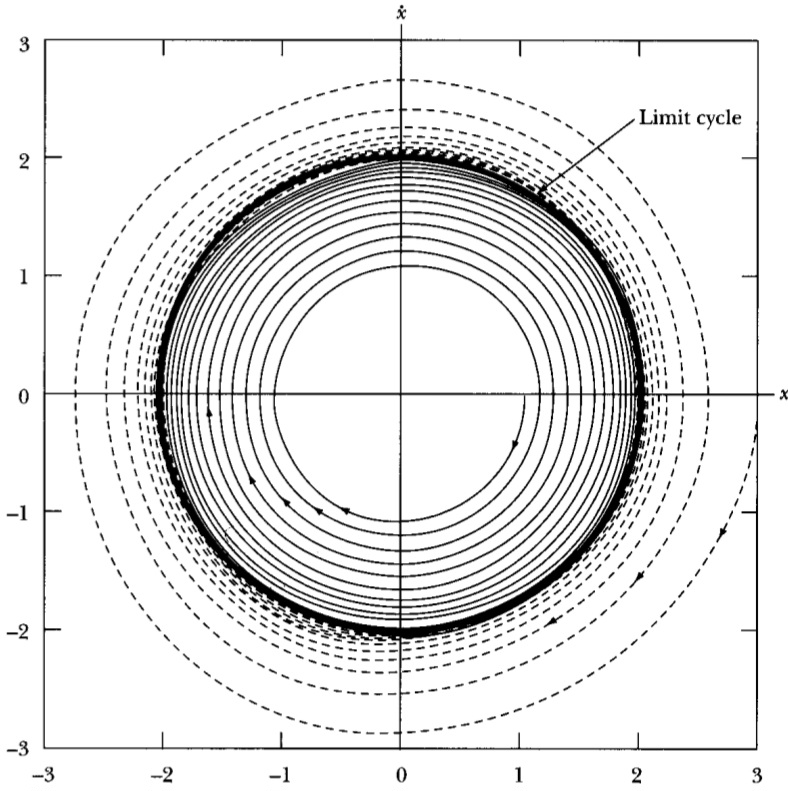
\includegraphics[width=0.5\linewidth]{figure3.1.jpg}
    \caption{반데르폴 진동자의 위상도이다. $\mu = 0.
    05, a=1, \omega_0=1$을 가정하였다. $\mu$가 아주 작으므로 limit cycle은 거의 원 모양이다. 실선으로 표현된 경로는 limit cycle 내부의 점 $(1, 0)$에서 출발하여 음의 감쇠력을 받는 경우를, 점선으로 표현된 경로는 limit cycle 외부의 점 $(3, 0)$에서 출발하여 양의 감쇠력을 받는 경우를 나타내었다.}
    \label{fig:3.1}
\end{figure}

한편 3.3절에서 배웠던 평면 진자의 위상도 역시 조사해 보자.\footnote{\href{https://en.wikipedia.org/wiki/Pendulum_(mechanics)}{영어 위키피디아 Pendulum (mechanics) 문서}의 example 문단을 참고하면 쉽게 이해할 수 있다.} 우리는 식 \ref{eq:3.7}과 식 \ref{eq:3.8}을 이용하여
\begin{equation}
    \dot{\theta} = \pm 2\sqrt{\frac{g}{l}} \left[ \frac{E}{2mgl} - \sin^2{\left(\frac{\theta}{2} \right)} \right]^{1/2}
    \label{eq:3.41}
\end{equation}
을 얻는다. 이는 $\theta$와 $\dot{\theta}$의 관계를 나타내므로, 이 식의 모양이 곧 위상도의 모양이 된다. 이를 통해 그려지는 위상도는 그림 \ref{fig3.2}를 참고하라. 식에서 알 수 있듯 위상도의 모양은 진자의 총 에너지 $E$와 관련되어 있다. 특히 $E=2mgl \equiv E_0$인 경우 식 \ref{eq:3.41}에 대입하면 위상도의 궤적은 코사인 함수가 되며, 이는 그림에 굵은 선으로 표시되어 있다. 후술하겠지만, $E=E_0$인 경우 진자는 이 선을 따라 운동하지 않는다.

\begin{figure}
    \centering
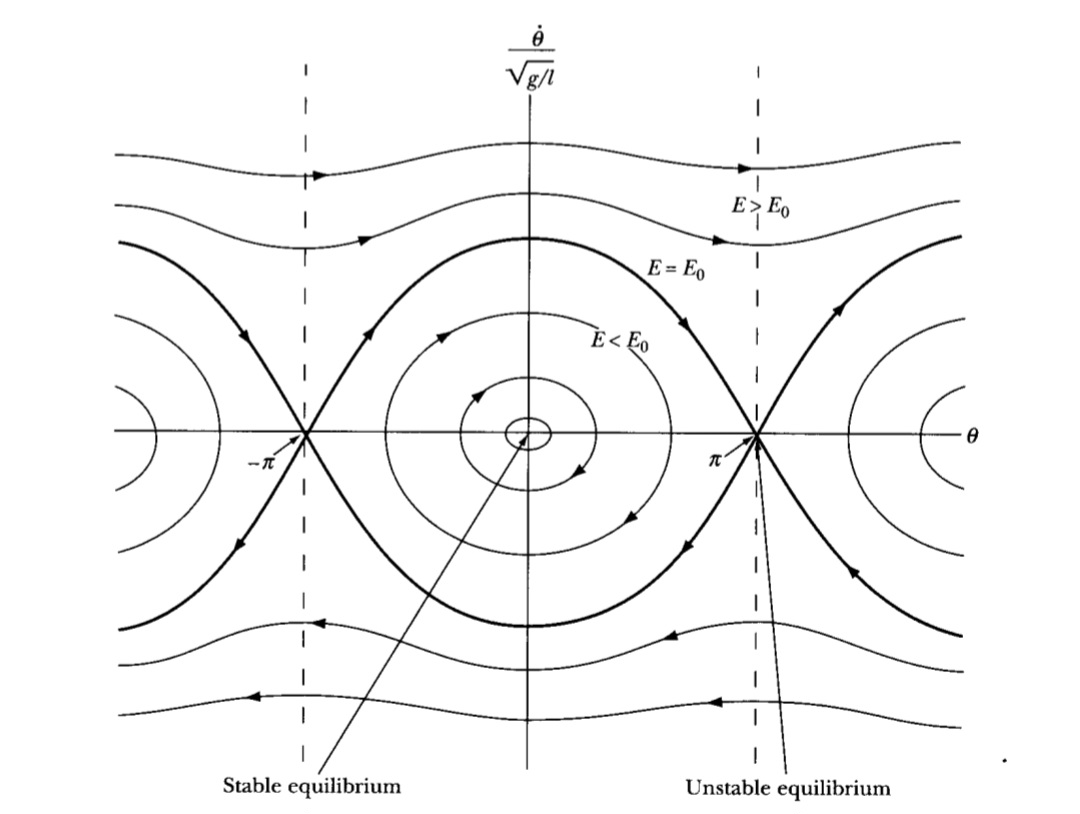
\includegraphics[width=1.0\linewidth]{figure3.2.jpg}
    \caption{평면 진자의 위상도이다. 평형점의 위치와 총 에너지 $E$의 크기에 따른 위상도 상의 궤적에 유의하라.}
    \label{fig3.2}
\end{figure}

이제 $E$의 크기에 따른 위상도의 모습을 구체적으로 조사하자. 먼저 $E < E_0$의 경우, 각 $\theta$가 충분히 작다면 우리는 식 \ref{eq:3.41}을
\begin{equation}
    \dot{\theta} = \pm 2\sqrt{\frac{g}{l}} \left[ \frac{E}{2mgl} - \frac{\theta^2}{4}\right]^{1/2}
    \label{eq:3.42}
\end{equation}
로 근사할 수 있다. 양변을 제곱하여 정리하면
\begin{equation}
    \dot{\theta}^2 + \frac{g}{l} \theta^2 = \frac{2E}{ml^2}
    \label{eq:3.43}
\end{equation}
이고, 이 식은 타원이므로 작은 진폭 영역에서 진자는 진동 운동을 한다. 이는 3.3절에서 배웠던 $0<k<1$인 경우와 동치이다. 각 $\theta$가 커질수록 이러한 근사의 정확성은 떨어지겠지만, 위상도 상의 궤적은 마찬가지로 폐곡선으로 나타날 것이다.

다음으로 $E > E_0$인 경우, 이는 $k>1$인 경우와 같으므로 진자는 최고점에 도달하고도 운동 에너지를 잃지 않는다. 즉, 연직 원운동을 한다. 따라서 위상도 상의 궤적은 폐곡선을 띠지 않으며, 단지 $\theta$가 커짐에 따라 주기적인 모양을 그린다.

마지막으로 $E = E_0$의 경우, 진자는 위상도 상의 궤적을 따라 운동하지 않는다. 우리는 $k=1$에서 주기가 무한대로 발산한다는 사실을 통해 이를 유추할 수 있다. 진자는 $\theta = -\pi, \pi, 3\pi \dots$인 지점, 즉 높이가 $2l$인 최고점에 정지해 있을 것이며, 이 상태에선 약간의 힘만 주어도 운동이 시작되므로 이는 불안정 평형에 해당한다. 이렇게 실제 운동을 표현하지는 않지만, 그 궤도를 기점으로 하여 계의 운동 양상이 바뀌는 궤도를 \textbf{분리 궤도(separatrix)}라고 한다.

limit cycle과 분리 궤도는 비선형계의 위상도에서만 나타나는 특징이다. 선형계의 위상도는 폐곡선 형태이거나, 한 지점으로 수렴하거나, 혹은 무한히 발산할 뿐이다. 하지만 비선형계의 위상도는 한 지점이 아닌 곡선에 수렴(limit cycle)하거나, 심지어는 여러 개의 영역으로 쪼개져(separatrix) 다양한 특이점을 가질 수도 있다는 사실을 말해 준다. 이들은 물리학의 마법진을 더욱 아름답게 만든다.

\section{더핑 진동자 (Duffing Oscillators)}
\textbf{더핑 진동자(Duffing oscillators)}는 운동 방정식
\begin{equation}
    \ddot{x} + \delta \dot{x} + \alpha x + \beta x^3 = \gamma \cos{(\omega t)}
\end{equation}
을 만족하는 계를 말한다. 이는 3.2절에서 다루었듯 복원력의 3차항까지 고려한 경우와 같다. 더핑 진동자는 복원력의 계수 $\alpha$와 $\beta$의 부호에 따라 세 가지로 분류된다. $\alpha > 0, \beta > 0$이면 계는 hard system이다. $\alpha > 0, \beta < 0$이면 계는 soft system이다. $\alpha <0, \beta >0$이면 계는 $x=0$에서 불안정 평형점을 갖고 좌우에 두 개의 안정 평형점을 갖는 구조가 된다.

일반적으로 더핑 진동자는 해석적인 해를 구할 수 없다. 그러나 우리는 어려운 문제의 해를 섭동론으로 근사할 수 있음을 배웠다. 컴퓨터를 이용한다면 더핑 진동자의 근사해를 충분한 정확도로 구할 수 있다.

더핑 진동자에선 \textbf{도약(jump)}과 \textbf{이력(hysteresis)} 현상이 나타난다. 도약은 구동력의 진동수를 서서히 변화시킬 때 시스템의 응답 진폭이 불연속적으로 튀는 현상이다. 우리는 공명 현상을 조사할 때 구동력의 진동수에 따른 진폭의 관계를 파악했다. 선형계에선 특정 진동수 $\omega$에 대해 계가 가질 수 있는 정상 상태의 진폭은 $A(\omega)$로 유일하게 결정되지만, 더핑 진동자에선 비선형 항 $\beta x^3$ 때문에 이것이 유일하게 결정되지 않는다. 따라서 진동수-진폭 곡선은 그림 \ref{fig:3.3}처럼 파도 모양으로 휘어지고, 특정 영역에서 여러 개의 진폭 값을 가지는 경우가 발생하게 된다.\footnote{곡선이 휘어지는 방향은 계의 성질과 관련되어 있다. soft system이라면 곡선은 왼쪽으로 휘어지고, hard system이라면 오른쪽으로 휘어진다.}

\begin{figure}
    \centering
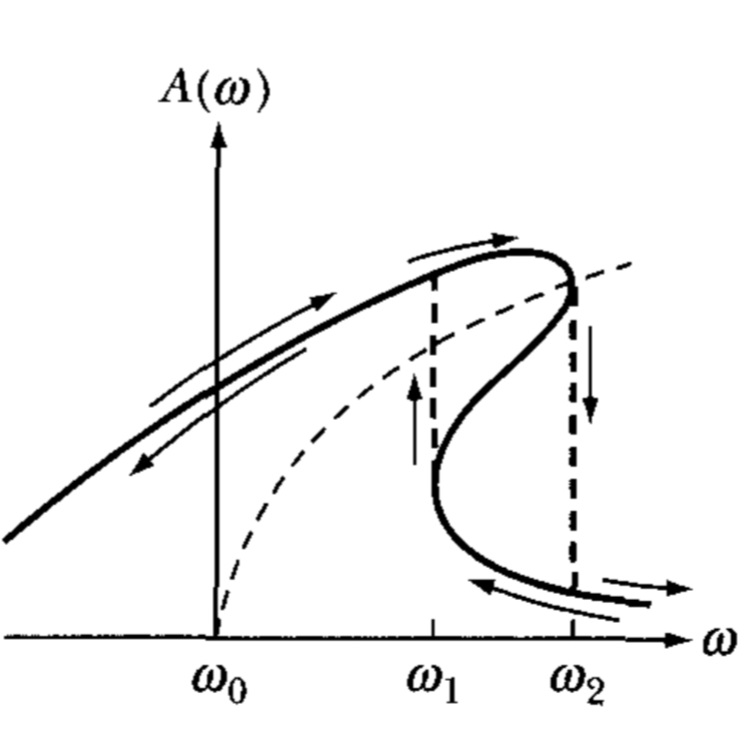
\includegraphics[width=0.4\linewidth]{figure3.3.jpg}
    \caption{hard system에서 진동수 $\omega$에 따른 진폭 $A(\omega)$를 나타내었다. $\omega_1$과 $\omega_2$에서 도약이 발생한다.}
    \label{fig:3.3}
\end{figure}

이제 $\omega$를 서서히 변화시켜 보자. 낮은 진동수에서 시작해 $\omega$를 서서히 올리면, 진폭은 곡선의 위쪽 안정 가지를 따라 완만하게 커진다. 하지만 곡선이 접히는 지점에 도달하면 진폭은 아래쪽 안정 가지로 급격히 추락한다. 반대로 높은 진동수에서 시작해 $\omega$를 서서히 내리면, 진폭은 아래쪽 안정 가지를 타고 내려오다가 수직 접선에 도달하는 순간 위쪽 안정 가지로 치솟는다. 이러한 추락과 상승이 바로 도약 현상이다.

다음으로 이력은 계가 과거 상태에 의존하여 현재 상태를 결정하는 현상을 말한다. $\omega$의 변화 과정을 다시 생각해 보자. 진동수를 올리고 내릴 때 진폭이 거치는 경로는 서로 다르므로, 이 경로를 이으면 닫힌 루프가 만들어진다. 그런데 더핑 진동자는 각 루프를 돌 때마다 과거의 상태(어느 가지에 있었는지)에 의존하여 현재 상태(어느 가지로 갈지)를 결정하므로 이력이 발생한다.

한편 특정한 더핑 진동자에선 카오스 현상이 발생한다. $\alpha <0, \beta > 0$인 경우, 특정 구동력이 주어지면 계는 초기 조건에 극도로 민감한 카오스 현상을 보인다. 그림 \ref{eq:3.4}를 참고하라. 다른 경우와 달리 $\gamma=0.50$에서 진동자의 변위 $x(t)$와 위상도는 불규칙적이다. 이는 카오스 현상의 특징이다.

위상도의 끌개가 프랙탈 구조를 가진다면\footnote{즉, 하우스도르프 차원(Hausdorff dimension)이 정수가 아니라면}, 우리는 이를 \textbf{야릇한 끌개(strange attractor)}라고 부른다. 예를 들어, $\gamma=0.50$의 위상도 상의 궤적은 서로 교차하지 않으면서 끝없이 층을 이룬다. 이를 시간 $t$가 주기 $T$의 정수배일 때만을 나타내는 \textbf{푸앵카레 단면(Poincaré section)}으로 잘라 보면, 무한히 확대해도 미세한 층상 구조가 반복되는 프랙탈 구조를 확인할 수 있다. 카오스 현상이 발생하는 계에선 야릇한 끌개가 나타난다.

\begin{figure}
    \centering
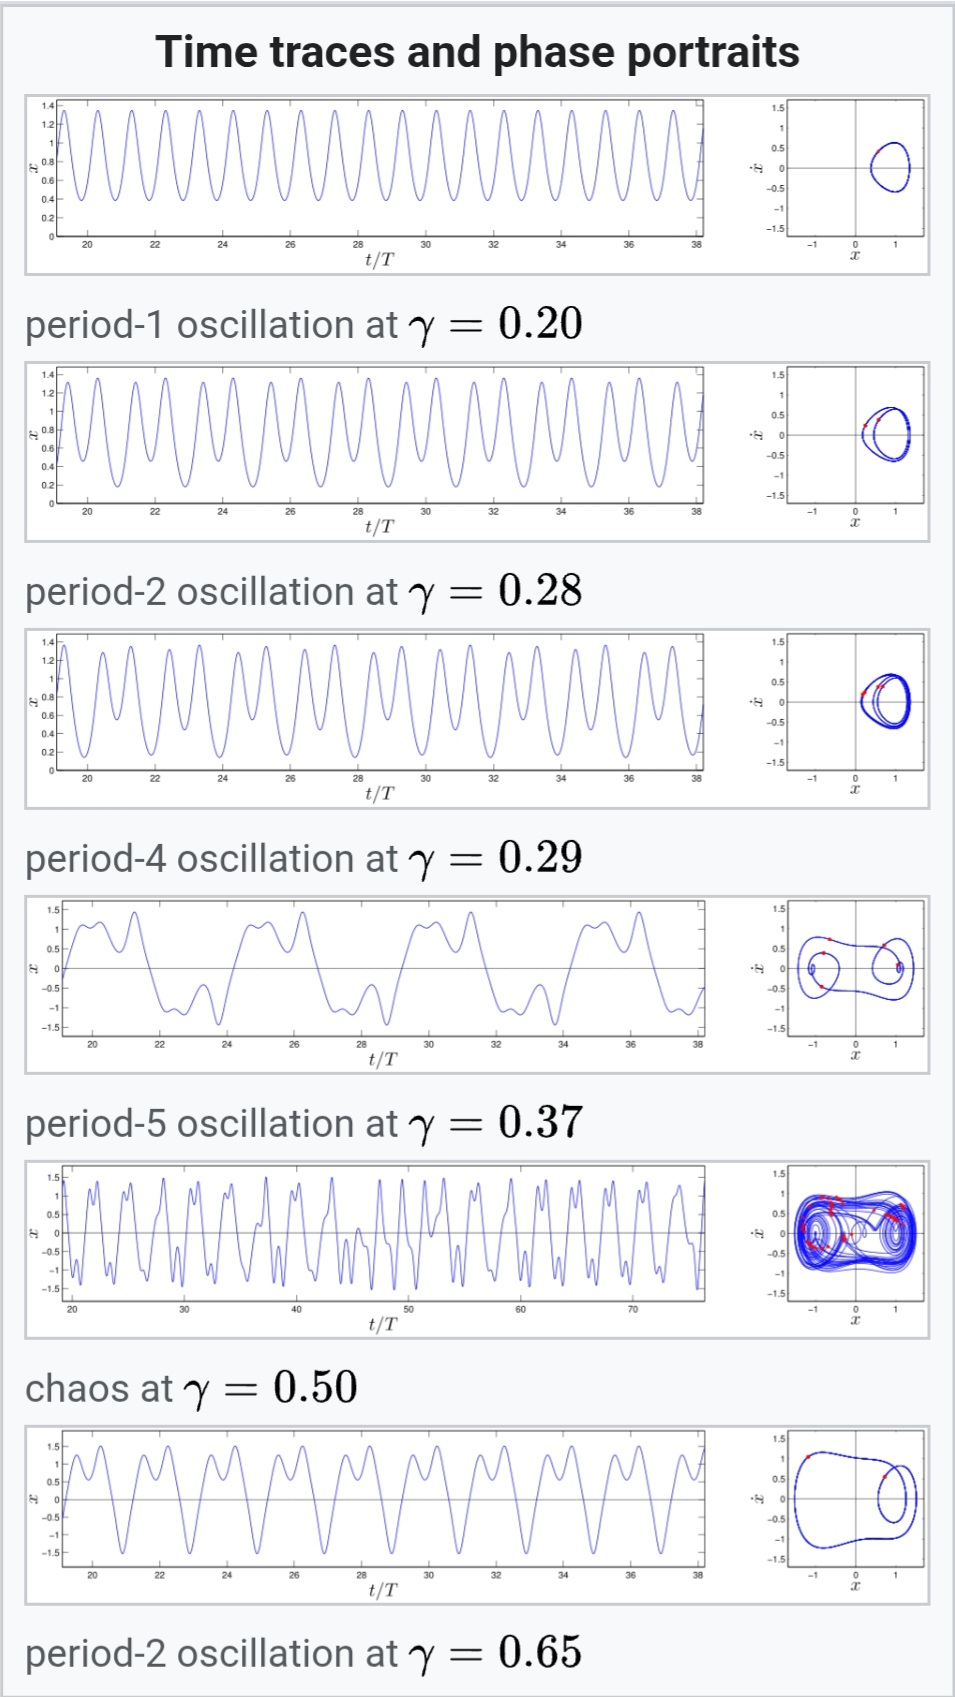
\includegraphics[width=0.6\linewidth]{figure3.4.jpg}
    \caption{더핑 진동자의 위상도이다. 왼쪽은 $x(t)$, 오른쪽은 위상도이다. $\gamma=0.50$에서 카오스 현상이 일어난다. 위상도 상의 빨간 점은 푸앵카레 단면으로, 시간 $t$가 주기 $T$의 정수배일 때마다 점을 찍은 것이다. \href{https://en.wikipedia.org/wiki/Duffing_equation}{출처: Wikipedia.}}
    \label{fig:3.4}
\end{figure}

이처럼 더핑 진동자는 우리가 지금까지 배웠던 여러 진동의 종합체이자 카오스 현상으로 이어지는 관문의 역할을 한다. 카오스 현상을 보이는 다른 비선형계로는 중심에서 구동력을 받는 진자, 이중 진자, 결합 진자, 자기 진자 등이 있다. 하지만 고전역학 수준에서 이를 모두 다루기엔 어려울 것이다. 그러니 비선형계와 카오스에 관한 마법은 이쯤에서 멈추도록 하자.

\newpage
% Chapter 4 시작
\chapter{중력 (Gravitation)}

\section{개요}
우리는 2장에서 힘에 대해 배웠다. 자연에는 네 가지의 기본 힘이 있다. 중력, 전자기력, 약한 핵력, 강한 핵력이 그것이다. 우리는 이 장에서 중력에 관하여 알아 보고자 한다.

뉴턴의 중력 법칙에 따르면, 두 질점 $m, M$은 서로를 끌어당기며 이 힘은 두 질점의 질량의 곱에 비례하고 거리의 제곱에 반비례한다. 즉, 수식으로 나타내면
\begin{equation}
    \mathbf{F} = -G\frac{mM}{r^2} \mathbf{\hat{r}}
    \label{eq:4.1}
\end{equation}
이다. 이때 $G$는 \textbf{중력 상수(gravitational constant)}라고 불리는 비례 상수이며 실험적으로 측정된다.\footnote{구체적인 방법은 캐번디시 실험(Cavendish Experiment)을 참고하라. 실험을 통해 얻은 중력 상수의 값은 약 $6.674 \times 10^{-11} \mathrm{N \cdot m^2kg^{-2}}$이다. 중력 상수의 유효 숫자는 다른 물리 상수들에 비해 작은데, 이는 중력이 매우 약한 힘이기 때문이다.} $r$은 두 질점 사이의 거리이며, $\mathbf{\hat{r}}$은 힘을 주는 질점에서 힘을 받는 질점으로의 방향을 가리키는 단위벡터이다. 마이너스 부호는 이들이 서로 끌어당긴다는 사실을 나타낸다. 한 질점이 다른 질점에 작용하는 힘의 방향이 두 질점을 연결한 선과 나란하므로 중력은 중심력이다.

식 \ref{eq:4.1}은 물체가 질점일 때에만 적용 가능하다. 만약 물체가 질점이 아니라 특정한 부피를 가지고 있다면 우리는 한 가지 가정을 더해야만 한다. 바로 중첩의 원리이다. 즉, 어떤 물체가 받는 중력은 다른 모든 물체가 그 물체에 주는 중력의 합과 같다. 특히 $M$의 연속적인 질량 분포를 가정하면 식 \ref{eq:4.1}은
\begin{equation}
    \mathbf{F} = -Gm\int_{\mathcal{V}} \frac{\rho( \mathbf{r'}) \mathbf{\hat{r}}}{r^2} \mathrm{d}\tau'
    \label{eq:4.2}
\end{equation}
처럼 쓸 수 있다. 이때 $\rho(\mathbf{r')}$은 $\mathbf{r'}$에서의 질량 밀도이며, $\mathrm{d}\tau'$은 질량 분포의 미소 부피 요소이다.

한편 단위 질량 당 작용하는 중력은 \textbf{중력장(gravitational field)}이라고 한다. 즉, 질량이 $m$인 질점이 중력을 받는다면 중력장 $\mathbf{g}$는
\begin{equation}
    \mathbf{g} = \frac{\mathbf{F}}{m} = -\frac{GM}{r^2} \mathbf{\hat{r}}
    \label{eq:4.3}
\end{equation}
을 만족한다. 중력장은 질량이 $M$인 원천 질점(source particle)이 고정되어 있을 때 질량이 $m$인 시험 질점(test particle)을 임의의 공간에 올려놓음으로써 측정된다. 따라서 원천 질점이 있는 점을 제외한 공간 전체에선 원천 질점에 의한 중력장이 형성된다. $M$의 연속적인 질량 분포를 가정하면 식 \ref{eq:4.3}은
\begin{equation}
    \mathbf{g} = -G\int_{\mathcal{V}} \frac{\rho( \mathbf{r'}) \mathbf{\hat{r}}}{r^2} \mathrm{d}\tau'
    \label{eq:4.4}
\end{equation}
이 된다.

중력장은 벡터장이므로 우리는 시험 질점이 받는 중력장의 방향을 연속적으로 연결한 역선(line of force)의 개념을 통해 이를 시각화할 수 있다. 몇 가지 역선의 예시는 그림 \ref{fig:4.1}을 참고하라.

\begin{figure}
    \centering
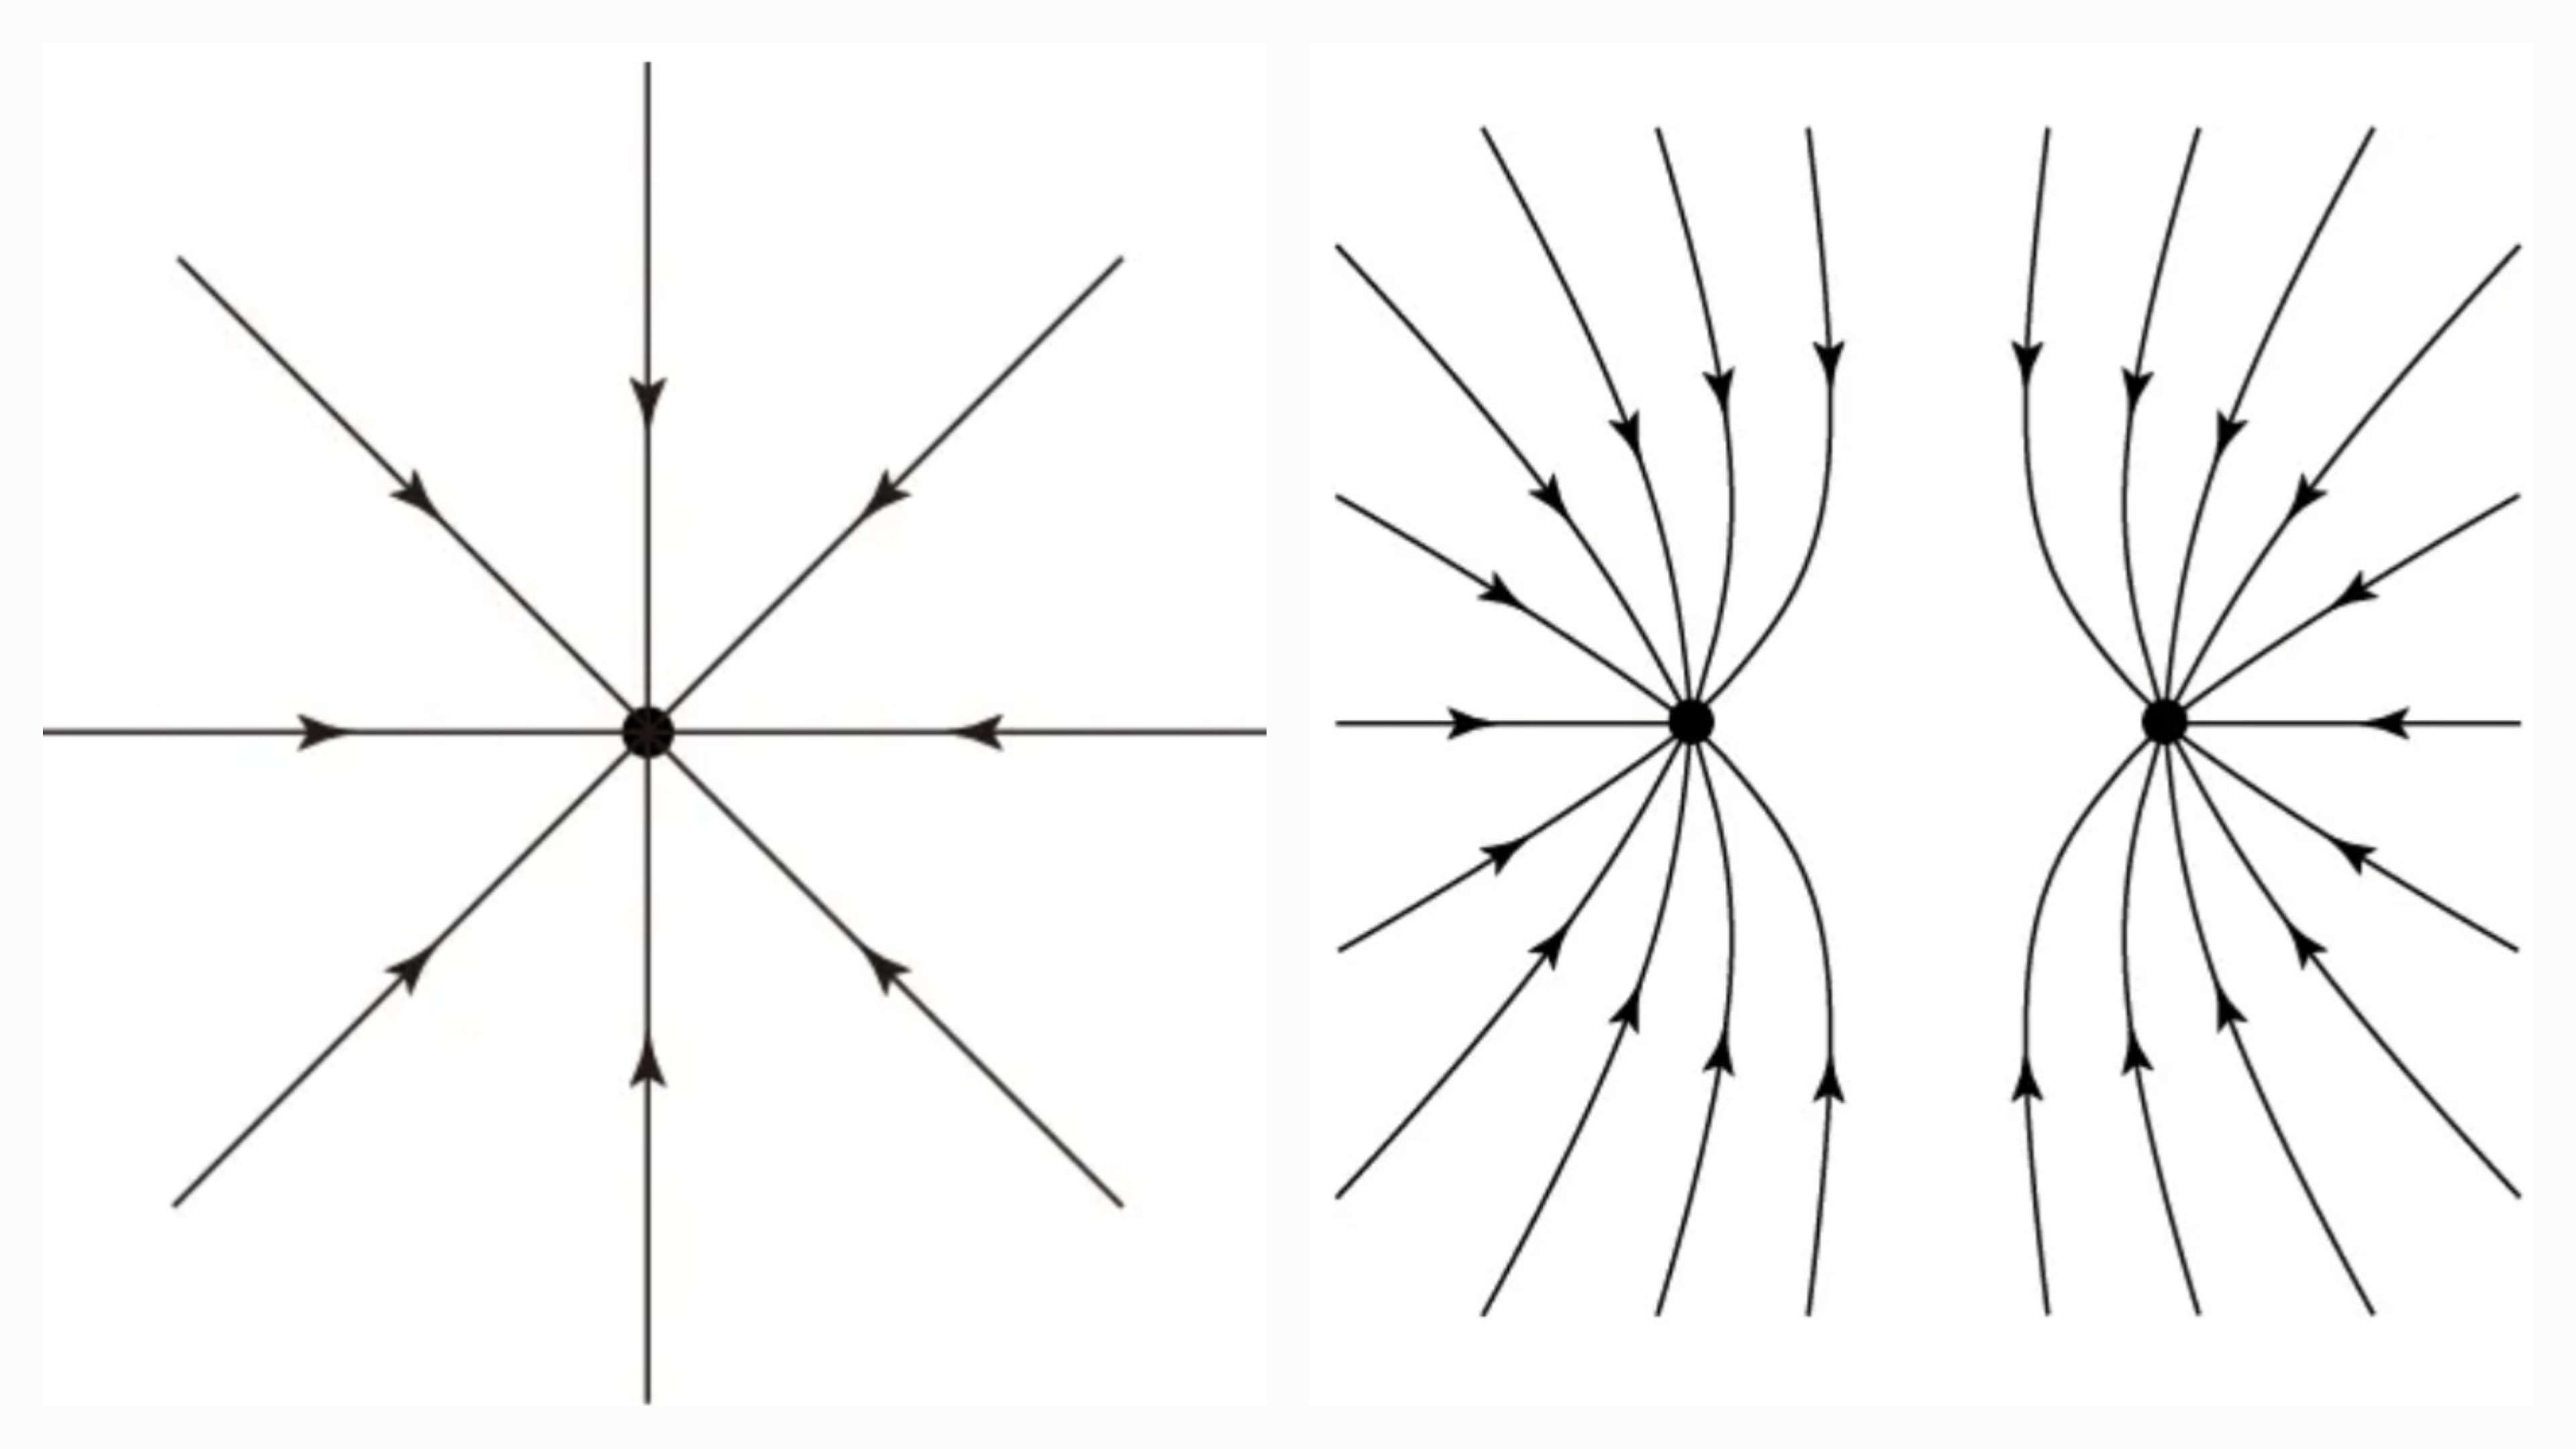
\includegraphics[width=0.6\linewidth]{figure4.1.jpg}
    \caption{중력장의 역선이다. 왼쪽은 한 원천 질점이 있을 때, 오른쪽은 두 원천 질점이 있을 때를 나타낸다.}
    \label{fig:4.1}
\end{figure}

\section{중력 퍼텐셜 (Gravitational Potential)}
식 \ref{eq:4.3}에서 보았듯 중력장은 $r^{-2}$에 비례한다. $\nabla \times (r^{-2} \mathbf{\hat{r}}) =0$이므로 $\nabla \times \mathbf{g}$도 0이다. 따라서 우리는 중력장을 스칼라 함수 $\Phi$의 그레이디언트로 표현할 수 있다. 즉,
\begin{equation}
    \mathbf{g} = -\nabla \Phi
    \label{eq:4.5}
\end{equation}
이다. 이렇게 정의되는 $\Phi$는 \textbf{중력 퍼텐셜(gravitational potential)}이 된다.

잠시 2.5절의 내용을 떠올려 보자. 우리는 보존장에서 비슷한 방식으로 퍼텐셜을 구했다. 이때 퍼텐셜은 그 자체로는 중요하지 않으며, 물리적 의미를 갖는 것은 항상 퍼텐셜의 차이였다. 그러므로 퍼텐셜 함수의 기준점은 임의로 결정될 수 있었다. 중력장 역시 보존장이므로, 편의를 위해 $r \to \infty$에서의 중력 퍼텐셜을 0으로 잡자. 이제 식 \ref{eq:4.5}를 적분하면
\begin{equation}
    \Phi = -\frac{GM}{r}
\end{equation}
이고, $M$의 연속적인 질량 분포를 가정하면
\begin{equation}
    \Phi = -G\int_{\mathcal{V}} \frac{\rho( \mathbf{r'})}{r} \mathrm{d}\tau'
\end{equation}
이다. 한편 $\mathbf{F} = - \nabla U$에 중력을 대입하면 퍼텐셜 에너지는
\begin{equation}
    U = -\frac{GmM}{r}
\end{equation}
이므로, 중력 퍼텐셜은
\begin{equation}
    U = m \Phi
\end{equation}
의 관계를 만족한다. 즉, 중력 퍼텐셜은 단위 질량 당 중력 퍼텐셜 에너지이다. 

중력장은 장의 일종이므로 \textbf{선속(flux)}의 개념을 도입할 수 있다. 원천 질점 $M$을 둘러싸는 폐곡면 $\mathcal{S}$를 고려하자. 간단하게 $\mathcal{S}$가 구 형태라고 가정하면, 구면을 통과하는 중력 선속 $F_g$는
\begin{equation}
    F_g = \int_{\mathcal{S}}\mathbf{g} \cdot \mathrm{d}\mathbf{a} = -GM\int_{0}^{2\pi} \int_{0}^{\pi} \sin{\theta} d\theta d\phi =-4\pi GM
\end{equation}
이 될 것이다. $\mathbf{g}$와 $d\mathbf{a}$가 서로 평행함을 명심하라. 놀랍게도 $\mathcal{S}$가 꼭 구가 아니더라도 임의의 폐곡면이기만 하면 $F_g$의 값은 $-4\pi GM$이다.\footnote{자세한 내용은 Griffiths 전자기학 4ed를 참고하라.} 따라서
\begin{equation}
    \int_{\mathcal{S}}\mathbf{g} \cdot \mathrm{d}\mathbf{a} = -4\pi GM
    \label{eq:4.11}
\end{equation}
이 성립하며, 이는 중력장의 \textbf{가우스 법칙(Gauss's law)}이 된다. 우변의 $M$은 폐곡면이 감싸고(enclosed) 있는 영역 속의 질량임을 유의하라.\footnote{이는 정전기학(Electrostatics)에서 전기장의 가우스 법칙과 정확히 같다. 전하 $q$를 질량 $M$으로, 비례 상수 $1/\epsilon_0$을 $-4\pi G$로 바꾸었을 뿐이다. 왜 이렇게 바뀌어야 할까? 뉴턴의 중력 법칙인 식 \ref{eq:4.1}과 정전기학의 쿨롱 법칙을 비교해 보아라. 사실 전기장의 가우스 법칙뿐만 아니라, 정전기학의 거의 모든 법칙은 이처럼 비례 상수만 바꾸면 중력장과 관련된 형태가 될 수 있다.}

한편 식 \ref{eq:4.11}에 발산 정리를 적용하면
\begin{equation}
    \int_{\mathcal{S}}\mathbf{g} \cdot \mathrm{d}\mathbf{a} = \int_{\mathcal{V}} (\nabla \cdot \mathbf{g}) \mathrm{d}\tau' = -4 \pi G \int_{\mathcal{V}} \rho \mathrm{d} \tau'
\end{equation}
이므로
\begin{equation}
    \nabla \cdot \mathbf{g} = -4 \pi G \rho
\end{equation}
가 성립하고, 이는 가우스 법칙의 미분형이 된다. 또한 $\mathbf{g} = -\nabla \Phi$이므로
\begin{equation}
    \nabla^2 \Phi = 4\pi G \rho
\end{equation}
이며, 이는 중력장의 \textbf{푸아송 방정식(Poisson's Equation)}이 된다. 우리는 이 편미분방정식을 풂으로써 계의 중력 퍼텐셜을 구할 수 있다.

많은 문제 상황에선 중력 퍼텐셜을 먼저 구하고 식 \ref{eq:4.5}를 이용해 중력장을 얻는 풀이가 편리하다. 중력 퍼텐셜을 먼저 구하는 것이 왜 좋을까? 중력 퍼텐셜은 중력장과 달리 스칼라이기 때문이다. 중력장은 벡터이므로, 우리는 물체가 받는 중력장을 좌표계의 각 성분별로 계산해야 한다. 그러나 중력 퍼텐셜을 먼저 구하면 마지막 그레이디언트 연산을 제외하고는 좌표계에 따른 성분을 전혀 고려할 필요가 없다. 물론 문제 상황에 대칭성이 존재하여 중력장의 방향을 미리 결정할 수 있다면, 중력장을 바로 구하는 것이 퍼텐셜을 먼저 구하는 것보다 더 쉬울 수도 있다. 따라서 실전에선 어떠한 접근이 더 편리한지 판단할 수 있는 능력이 중요하다.

\section{구각 정리 (Shell Theorem)}
중력 퍼텐셜의 개념을 활용하여 그림 \ref{fig:4.2}처럼 균일한 밀도 $\rho$를 가지는 구각(spherical shell)의 중력장을 구해 보자. 구각의 외부 반지름은 $a$, 내부 반지름은 $b$이다.

먼저 구각의 외부 영역 $R>a$부터 조사하자. 이 경우 중력 퍼텐셜은
\begin{equation}
\begin{aligned}
    \Phi &= -G \int_{\mathcal{V}} \frac{\rho(r')}{r} d\tau' \\
    &= - G \rho \int_b^a r'^2 dr' \int _0^{\pi} \frac{\sin{\theta}}{r} d\theta \int_0^{2\pi} d\phi \\
    &= -2\pi G \rho \int_b^a r'^2 dr' \int _0^{\pi} \frac{\sin{\theta}}{r} d\theta 
\end{aligned}
\end{equation}
이다. 이때
\begin{equation}
\begin{aligned}
    r^2 &= r'^2 + R^2 - 2r' R \cos{\theta} \\
    2rdr &= 2r'R \sin{\theta} d\theta
\end{aligned}
\end{equation}
이므로
\begin{equation}
    \int \frac{\sin{\theta}}{r} d\theta = \int \frac{1}{r'R} dr
\end{equation}
가 성립한다. 따라서
\begin{equation}
\begin{aligned}
    \Phi &= -\frac{2\pi G \rho }{R} \int_b^a r' dr' \int _{r_{\mathrm{min}}}^{r_{\mathrm{max}}} dr
\end{aligned}
\end{equation}
이고, $R>a$에서 $r_{\mathrm{max}}, r_{\mathrm{min}}$의 값은 각각 $R+r', R-r'$이므로 중력 퍼텐셜은
\begin{equation}
    \begin{aligned}
        \Phi (R > a) &= -\frac{2\pi G \rho }{R} \int_b^a r' dr' \int _{R-r'}^{R+r'} dr \\
        &= -\frac{4\pi G \rho }{R} \int_b^a r'^2 dr' \\
        &= -\frac{4\pi G \rho }{3R}(a^3-b^3) \\
        &= -\frac{GM}{R}
    \end{aligned}
\end{equation}
가 된다. 여기서 $M$은 구각의 질량이다. 구각 외부의 경우, 구각이 만드는 중력 퍼텐셜은 질량 $M$인 질점이 구각의 중심에 놓여 있을 때 만드는 중력 퍼텐셜과 같다.

\begin{figure}
    \centering
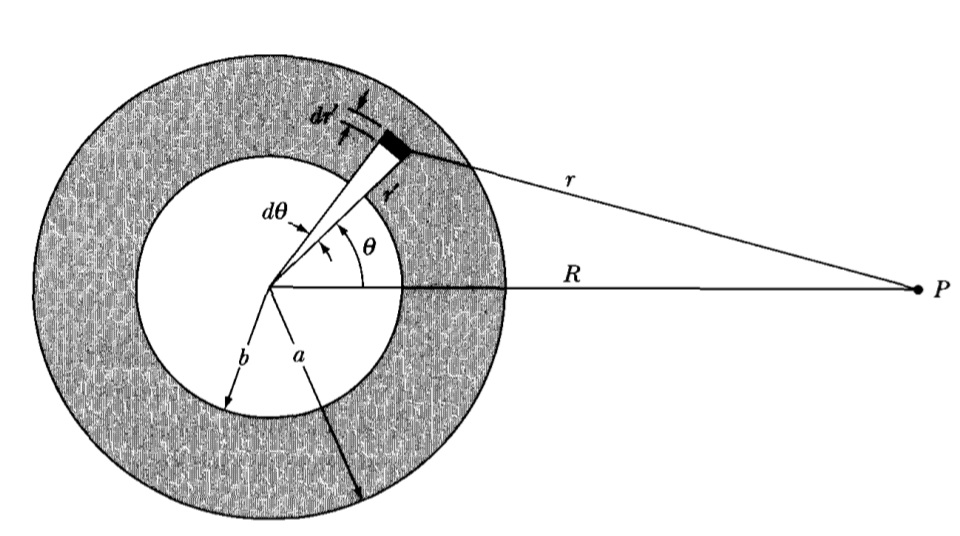
\includegraphics[width=0.7\linewidth]{figure4.2.jpg}
    \caption{구각 정리를 설명하는 그림이다.}
    \label{fig:4.2}
\end{figure}

다음으로 조사할 것은 공동의 내부 영역 $R < b$이다. 이 경우 $r_{\mathrm{max}}, r_{\mathrm{min}}$의 값은 각각 $r'+R, r'-R$이므로
\begin{equation}
    \begin{aligned}
        \Phi (R < b) &= -\frac{2\pi G \rho }{R} \int_b^a r' dr' \int _{r'-R'}^{r'+R} dr \\
        &= -4\pi G \rho \int_b^a r' dr' \\
        &= -2\pi G \rho (a^2-b^2)
    \end{aligned}
\end{equation}
을 얻는다. 공동 내부의 경우, 구각이 만드는 중력 퍼텐셜은 일정하다.

마지막으로 구각의 내부 영역 $b < R < a$를 조사하자. 이 경우 구각은 $R$의 내부와 $R$의 외부 두 가지 영역으로 나누어지므로, 중력 퍼텐셜은 이들의 합인
\begin{equation}
    \begin{aligned}
        \Phi(b < R < a) &= -\frac{4\pi G \rho }{3R}(R^3-b^3) - 2\pi G \rho (a^2-R^2) \\
        &= - 4\pi G \rho \left( \frac{a^2}{2} - \frac{b^3}{3R} - \frac{R^2}{6} \right)
    \end{aligned}
\end{equation}
가 된다. 이상의 결과를 종합하고 식 \ref{eq:4.5}를 통해 중력장을 구하면
\begin{equation}
    \begin{aligned}
        \mathbf{g} (R > a) &= -\frac{GM}{R^2} \mathbf{\hat{R}} \\
        \mathbf{g} (b < R < a) &= -\frac{4 \pi G \rho}{3} \left(R- \frac{b^3}{R^2} \right) \mathbf{\hat{R}} \\
        \mathbf{g} (R < b) &= \mathbf{0}
    \end{aligned}
    \label{eq:4.22}
\end{equation}
이다. 중력 퍼텐셜과 중력장의 그래프는 그림 \ref{fig:4.3}에 나와 있다.

\begin{figure}
    \centering
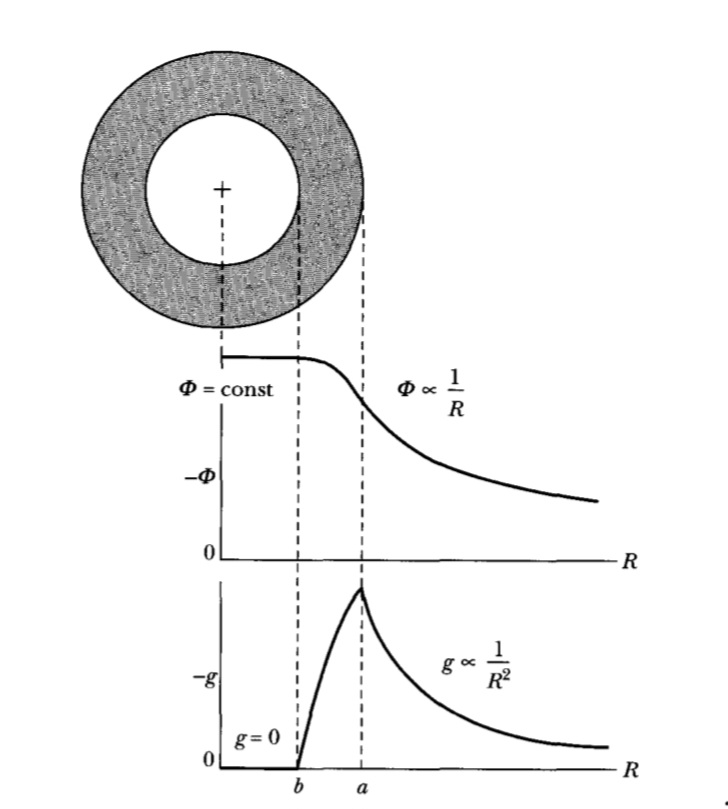
\includegraphics[width=0.6\linewidth]{figure4.3.jpg}
    \caption{구각 정리의 결과로 얻는 중력 퍼텐셜과 중력장의 크기를 나타낸 그래프이다. 공동 내부에서 중력장의 크기는 0(무중력 상태)임을 기억하라.}
    \label{fig:4.3}
\end{figure}

한편 우리는 가우스 법칙을 이용하여 중력장을 구할 수도 있다. 폐곡면 $\mathcal{S}$를 반지름이 $R$인 구면으로 잡자. 먼저 구각 외부의 경우, $R>a$이므로 $\mathcal{S}$가 감싸는 질량은 $M$이고 식 \ref{eq:4.11}의 우변은 $-4\pi R M$이다. 다음으로 공동 내부의 경우, $R<b$이므로 $\mathcal{S}$가 감싸는 질량은 0이고 식 \ref{eq:4.11}의 우변은 0이다. 마지막으로 구각 내부의 경우, $\mathcal{S}$가 감싸는 질량은 $\frac{4}{3} \pi (R^3 - b^3) \rho$이고 식 \ref{eq:4.11}의 우변은 $-\frac{16}{3} \pi^2 G \rho (R^3 - b^3)$이다. 각각의 경우를 계산하면 식 \ref{eq:4.22}와 같은 결과를 얻는다.

구각 정리의 결과는 다양하게 응용된다. 예를 들어 속이 꽉 찬 구가 만드는 중력장을 구하고자 하는 경우, 우리는 간단히 식 \ref{eq:4.22}에 $b \to 0$의 극한을 취하여
\begin{equation}
    \begin{aligned}
        \mathbf{g}(R>a) &= -\frac{GM}{R^2} \mathbf{\hat{R}} \\
        \mathbf{g}(R<a) &= -\frac{4 \pi G \rho R}{3} \mathbf{\hat{R}}
    \end{aligned}
\end{equation}
을 얻을 수 있다. 따라서 속이 꽉 찬 구가 만드는 중력장은 구 외부의 경우 질량 $M$인 질점이 구의 중심에 놓여 있을 때와 같고, 구 내부의 경우 $R$에 비례한다. 한편 반지름 $a$인 구 표면에만 질량이 균일한 면밀도 $\sigma$로 분포할 때에도, 우리는 간단히 $b \to a$의 극한을 취하여
\begin{equation}
    \begin{aligned}
        \mathbf{g}(R>a) &= -\frac{GM}{R^2} \mathbf{\hat{R}} \\
        \mathbf{g}(R<a) &= \mathbf{0}
    \end{aligned}
\end{equation}
를 얻을 수 있다. 의문이 든다면 적분을 통해 중력 퍼텐셜을 직접 구해 보아라. 구 표면이 만드는 중력장은 구 외부의 경우 질량 $M$인 질점이 구의 중심에 놓여 있을 때와 같고, 내부의 경우 영벡터가 된다.

구각 정리의 결과를 응용하고자 한다면, 중력장은 불연속일 수 있지만 중력 퍼텐셜은 항상 연속이어야 한다는 사실을 기억하라. 중력 퍼텐셜이 불연속이라면 불연속점에서 중력의 크기가 무한대여야 하지만, 이는 물리적으로 불가능하다.

\section{조석력 (Tidal Forces)}
중력은 주로 천체와 같이 막대한 질량을 가진 물체 사이에서 위용을 드러낸다. 우주 단위로 가면 중력은 가장 보편적인 힘이나 다름없다. 우리는 이 절에서 중력에 의한 현상의 예시로 달이 지구에 만드는 조석 현상을 보고자 한다.

조석 현상은 한 천체 내에서 위치에 따른 중력의 차이가 생기기 때문에 발생한다. 편의를 위해 지구가 완벽한 구형이며 표면이 모두 물로 덮여 있다고 가정하자. 또 달과 지구를 제외한 외부 천체의 영향을 배제하고, 지구의 회전과 마찰 역시 무시하자.

계산에 앞서 주의해야 할 점은 지구 자체와 그 표면의 물이 각각 달의 중력에 의해 서로 다른 가속을 받고 있다는 것이다. 즉, 지구의 질량중심을 좌표계의 원점으로 놓는다면 비관성 좌표계가 된다. 그러므로 우리는 그림 \ref{fig:4.4}와 같이 관성 좌표계 $x', y', z'$을 잡고 가속도의 차이를 계산할 것이다.

\begin{figure}
    \centering
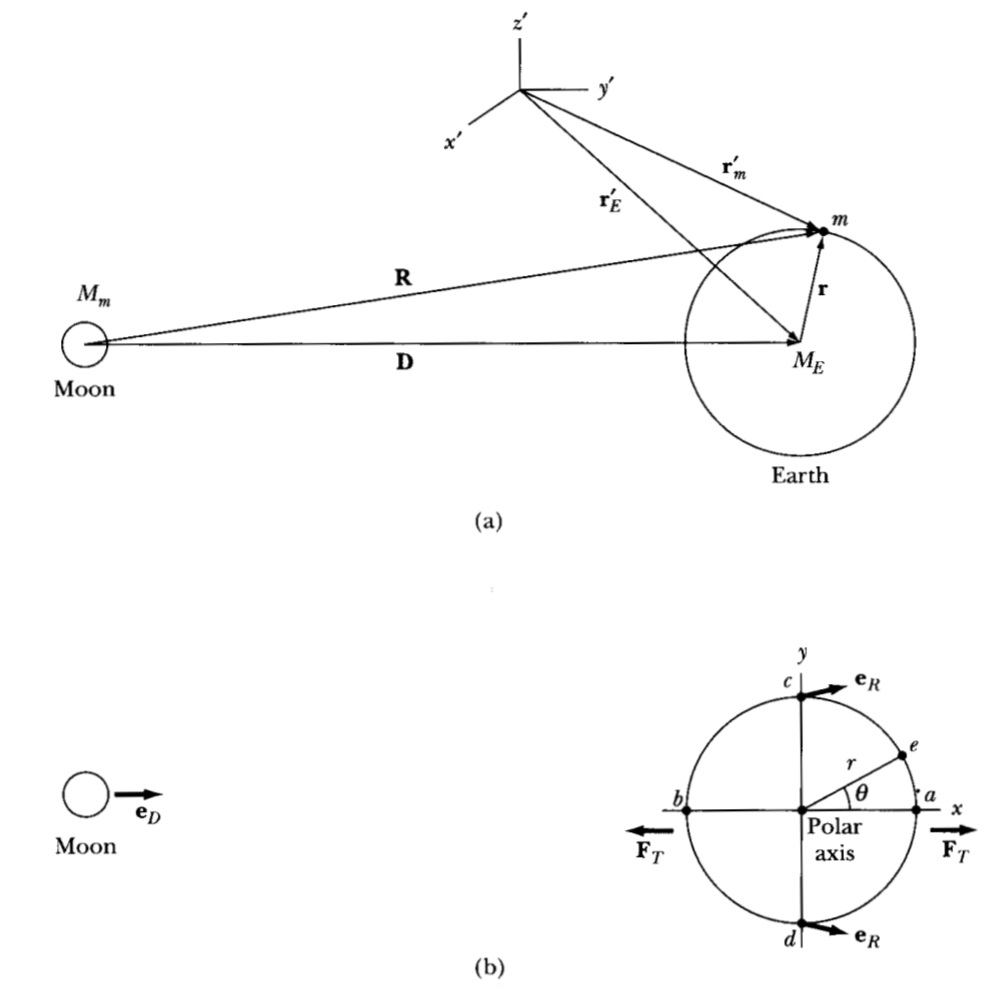
\includegraphics[width=0.7\linewidth]{figure4.4.jpg}
    \caption{조석력을 설명하는 그림이다. (a)는 문제 상황의 모식도이며, (b)는 각 벡터의 방향을 극좌표계 위에 나타내었다.}
    \label{fig:4.4}
\end{figure}

지구의 질량을 $M_E$, 지구의 질량중심의 위치를 $\mathbf{r'}_E$, 달의 질량을 $M_M$이라고 하자. 달의 질량중심에서 지구의 질량중심으로 향하는 위치벡터는 $\mathbf{D}$이다. 이제 질량 $m$인 물 입자가 지구 표면 상의 지점 $\mathbf{r'}_M$에 위치해 있고, 이 지점은 지구의 질량중심으로부터 $\mathbf{r}$, 달의 질량중심으로부터 $\mathbf{R}$만큼 떨어진 곳이라고 하자. 관성 좌표계에서 물 입자가 받는 중력은 다음과 같다.
\begin{equation}
    m\mathbf{\ddot{r}}'_m = -\frac{GmM_E}{r^2}\mathbf{\hat{r}} - \frac{GmM_M}{R^2}\mathbf{\hat{R}}
\end{equation}
비슷하게, 지구의 질량중심이 달에 의해 받는 중력은
\begin{equation}
    M_E\mathbf{\ddot{r}}_E = -\frac{GmM_M}{D^2}\mathbf{\hat{D}}.
\end{equation}
우리가 구하고자 하는 건 지구의 질량중심을 원점으로 하는 비관성 좌표계에 대한 물 입자의 가속도 $\mathbf{\ddot{r}}$이다. 이는
\begin{equation}
    \mathbf{\ddot{r}} =\mathbf{\ddot{r}}'_m - \mathbf{\ddot{r}}_E
\end{equation}
이므로, 앞선 결과를 대입하여
\begin{equation}
\begin{aligned}
    \mathbf{\ddot{r}} &= -\frac{GM_E}{r^2}\mathbf{\hat{r}} - \frac{GM_M}{R^2}\mathbf{\hat{R}} + \frac{GM_M}{D^2}\mathbf{\hat{D}} \\
    &= \frac{GM_E}{r^2}\mathbf{\hat{r}} - GM_M \left( \frac{\mathbf{\hat{R}}}{R^2} - \frac{\mathbf{\hat{D}}}{D^2} \right)
\end{aligned}
\label{eq:4.28}
\end{equation}
를 얻는다. 식 \ref{eq:4.28}의 첫째 항은 지구의 중력이며, 둘째 항은 조석 현상을 일으키는 \textbf{조석력(tidal force)} $\mathbf{F}_T$가 된다.

이제 지구 표면의 몇몇 지점에서 조석력의 크기와 방향을 조사해 보자. 먼저 그림 \ref{fig:4.4}(b)의 점 a는 달에서 가장 멀리 떨어진 지점이다. 이곳에선 $\mathbf{\hat{D}}$와 $\mathbf{\hat{R}}$의 뱡향이 $x$축으로 같으며 $\mathbf{R} = \mathbf{D} + \mathbf{r}$가 성립한다. $(r/D) \ll 1$를 가정하면, 조석력은
\begin{equation}
\begin{aligned}
    F_{T_x} &= -GmM_M \left( \frac{1}{R^2} - \frac{1}{D^2} \right) \\
    &= -GmM_M \left( \frac{1}{(D+r)^2} - \frac{1}{D^2} \right) \\
    &= -\frac{GmM_M}{D^2} \left( \frac{1}{(1+(r/D))^2} - 1 \right) \\
    &\approx -\frac{GmM_M}{D^2} \left( 1-2\frac{r}{D}- 1 \right) = \frac{2GmM_Mr}{D^3}
\end{aligned}
\label{eq:4.29}
\end{equation}
으로 나타낼 수 있다. 첨자 $T_x$는 조석력의 $x$성분을 표현한 것이며, 마지막 줄에서 $(1+x)^{-2}$의 테일러 전개를 사용했다.\footnote{실제 값을 대입해 보면, $(r/D) \approx 0.02$ 정도이다.}

다음으로 점 c를 조사하자. 이곳에선 $\mathbf{D}$와 $\mathbf{R}$의 방향이 정확히 같지 않지만, $R \approx D$이므로 각각의 $x$성분은 비슷한 값을 가진다. 따라서 조석력의 $x$성분은 근사적으로 상쇄된다. 한편 $\mathbf{\hat{R}}$의 $y$성분은 0이고 $\mathbf{\hat{D}}$의 $y$성분은 $(r^2 / \sqrt{D^2 + r^2}) \approx (r/D)$이므로
\begin{equation}
    F_{T_y} = -\frac{GmM_M r}{D^3}
\end{equation}
이다.

이상의 결과를 종합하면, 점 e와 같이 지구 표면의 임의의 지점에서 나타나는 조석력은 다음과 같다.
\begin{equation}
    \begin{aligned}
        F_{T_x} &= \frac{2GmM_Mx}{D^3} = \frac{2GmM_Mr\cos{\theta}}{D^3} \\
        F_{T_y} &= -\frac{GmM_xy}{D^3} = -\frac{GmM_Mr\sin{\theta}}{D^3}
    \end{aligned}
    \label{eq:4.31}
\end{equation}
식 \ref{eq:4.31}은 $x$축을 장축으로 하는 타원을 그리므로, 지구 표면의 물은 타원형으로 분포하려는 힘을 받는다. 그 중에서도 그림 \ref{fig:4.4}(b)의 점 a와 b는 가장 강한 힘을 받는 지점이며 만조 현상이 발생한다. 반면 점 c와 점 d는 가장 약한 힘을 받는 지점이며 간조 현상이 발생한다. 실제로 지구는 자전하기 때문에 우리는 하루에 두 번씩 만조와 간조 현상을 겪는다.\footnote{예를 들어 그림 \ref{fig:4.4}(b)의 점 b에 위치한 도시가 있다고 해 보자. 자전이 반시계 방향이라면 도시는 약 12시간 후 점 d를 거쳐 점 a에 있게 되며, 다시 약 12시간이 흐른 후 점 c를 거쳐 점 b로 돌아오게 된다. 이때 각 점들은 달에 대한 상대 위치임에 유의하라. 한편 만조 사이의 시간 간격은 정확히 12시간이 아닌데, 이는 달이 지구를 공전하기 때문이다. 지구에 대한 달의 공전은 27.3일을 주기로 한다. 즉, 달은 하루에 $(360^{\circ}/27.3) \approx 13.2^{\circ}$를 돈다. 그러므로 달이 지구에 대해 전날과 같은 상대 위치를 보이려면 지구는 $(24\mathrm{h} / 360^{\circ}) \times 13.2^{\circ} \approx 52.8$분을 더 돌아야 하고, 만조 현상은 하루에 두 번 발생하므로 만조 사이의 시간 간격은 약 12시간 26분이 된다.}

조석력을 명시적으로 구했으므로, 우리는 조수간만의 차 역시 계산할 수 있다. 만조인 지점 점 a와 간조인 지점 점 c의 해수면의 차를 $h$로 두자. 질량이 $m$인 물 입자를 점 c에서 점 a로 이동시키는데 드는 일 $W$는
\begin{equation}
    \begin{aligned}
        W &= \int_r^0 F_{T_y } dr +  \int_0^r F_{T_x } dr \\
        &= \frac{GmM_M}{D^3} \int_r^0 (-y) dy +  \int_0^r 2x dx \\
        &= \frac{3GmM_Mr^2}{2D^3}
    \end{aligned}
\end{equation}
이다. 이때 일의 경로는 계산의 편의를 위해 지구의 질량중심을 거치는 수직 경로를 취했다. 한편 점 a와 점 c에 위치한 물 입자의 퍼텐셜 에너지 차이는 $mgh$이므로, $W=mgh$를 풀면
\begin{equation}
    h = \frac{3GM_Mr^2}{2gD^3}
\end{equation}
을 얻는다. 실제 값을 대입해 보면 $h \approx 0.54$
m이다. 물론 조수간만의 차는 지형의 영향을 크게 받기 때문에, 이는 현실에서 유용하게 쓰이는 값은 아니다.

한편 우리는 천체가 받는 중력과 조석력의 크기를 비교하여 흥미로운 현상을 확인할 수 있다. 식 \ref{eq:4.28}을 보자. 만약 어떤 물체가 받는 조석력이 그 물체가 속한 천체의 중력보다 크다면, 물체는 천체에서 떨어져 나갈 것이다. 즉, 천체는 갈기갈기 찢어져 붕괴한다. 우리는 이 붕괴 지점을 \textbf{로슈 한계(Roche limit)}라고 부른다.

로슈 한계는 주로 위성이 모성의 중력에 의한 조석력에 의해 파괴되지 않고 접근할 수 있는 한계를 설명할 때 등장한다. 모성의 질량을 $M_p$, 위성의 질량을 $M_s$라고 하자. 조석력이 식 \ref{eq:4.29}와 같을 경우, 로슈 한계에선
\begin{equation}
    \frac{GM_s}{r^2} = \frac{2GmM_pr}{D^3}
\end{equation}
이 성립하므로, $d$에 대해 풀면
\begin{equation}
    d = r_s \left( \frac{2M_p}{M_s} \right)^{1/3}
    \label{eq:4.35}
\end{equation}
을 얻는다. 조석력을 주는 천체가 달에서 모성으로 바뀌었으므로 $M_M$은 $M_p$에, 조석력을 받는 천체가 지구에서 위성으로 바뀌었으므로 $M_E$는 $M_s$에 대응됨을 유의하라. 천체의 질량을 부피와 밀도의 곱으로 표현하면 식 \ref{eq:4.35}는
\begin{equation}
    d = r_p \left( \frac{2 \rho_p}{\rho_s} \right)^{1/3} \approx 1.26R\left( \frac{\rho_p}{\rho_s} \right)^{1/3}
\end{equation}
처럼 쓸 수 있다. 이는 강체 위성에 대한 로슈 한계이며, 실제로 위성은 유체의 성질을 띨 수 있으므로 앞에 붙는 계수는 위성의 물성에 따라 바뀔 수 있다.\footnote{유체 위성에 대한 로슈 한계는 $2.44R$의 계수를 적용한다.} 로슈 한계는 토성을 장식하는 고리의 생성 원리나 1994년 목성에 충돌한 슈메이커-레비 9 혜성의 붕괴 등을 잘 설명한다.

\newpage
% Chapter 5 시작
\chapter{변분법 (Calculus of Variations)}

\section{개요}
우리는 지금까지 뉴턴 역학에 관해 배웠다. 뉴턴 역학의 철학은 인과론적 세계관이다. 즉, 힘이 주어지면 물체는 운동한다. 힘은 원인이고 운동은 결과다. 그러나 자연 현상을 바라보는 방법에는 다른 철학 역시 존재한다. 바로 인과론적 세계관이다. 이에 따르면 자연은 매 순간 힘에 떠밀려 억지로 움직이는 것이 아니라, 시작점과 끝점 사이의 가능한 모든 경로들 중에서 어떤 특별한 물리량을 최적화(최소화)하는 경로를 찾아 스스로 움직인다.

\textbf{변분법(calculus of variations)}은 이처럼 최적화 문제를 다루기 위해 고안된 수학적 기법이다. 함수 자체를 변수로 삼아 함수의 최적 경로를 찾아내는 이 강력한 수학적 기법은 후에 해석역학이라는 고전역학의 새 지평을 열게 된다.

이 장에서 우리는 해석역학의 서곡으로 변분법의 수학적 토대를 배운다. 이 장의 내용을 완벽히 이해한다면, 우리는 운동 방정식을 우아하게 세워 나가는 해석역학의 놀라운 마법을 비로소 감상할 수 있게 될 것이다.

\section{변분법의 기본 보조정리 (Fundamental Lemma of Calculus of Variations)}
연속함수 $f:[a, b] \to \mathbb{R}$와, $c \notin (a, b)$에 대해 $\eta(c) = 0$인 임의의 매끄러운 함수 $\eta$를 고려하자. 만약
\begin{equation}
    \int_a^b f(x) \eta(x) \mathrm{d}x = 0
    \label{eq:5.1}
\end{equation}
이면, $\forall x \in [a, b]$에 대해 $f(x) = 0$이다. 이것이 바로 \textbf{변분법의 기본 보조정리(fundamental lemma of calculus of variations)}이며, 앞으로 나올 오일러-라그랑주 방정식의 유도에 있어 핵심적인 보조정리가 된다.

증명해 보자. $f(x) = 0$이 성립하지 않는다고 가정하면, $x_0 \in [a, b]$에 대해 $f(x_0) \neq 0$일 것이다. 일반성을 잃지 않고 $f(x_0) > 0$이라고 하자.\footnote{$f(x_0) < 0$이어도 같은 논리가 적용된다. 이 경우 식 \ref{eq:5.3}의 값은 음수가 되고, 모순이 발생한다.} $f$가 연속함수이므로 우리는 $x_0$ 근처의 적당한 구간 $[c, d] \subset [a, b]$를 잡아 $f(x) > 0$이 되게 할 수 있다. 이때 $c \leq x_0 \leq d$이다. 이제 $\eta(x)$의 시험 함수(test function)를
\begin{equation}
    \eta(x) = \begin{cases}
    (x-c)^2 (x-d)^2 & (c<x<d) \\
    0 & \mathrm{otherwise} \end{cases}
    \label{eq:5.2}
\end{equation}
로 두자. $\eta$는 임의의 매끄러운 함수이므로 이 함수에 대해서도 식 \ref{eq:5.1}이 성립해야 한다. 그런데 $\eta(x) = 0$인 구간을 제외하면
\begin{equation}
    \int_a^b f(x) \eta(x) \mathrm{d}x = \int_c^d f(x) (x-c)^2 (x-d)^2 \mathrm{d}x
    \label{eq:5.3}
\end{equation}
이고, 구간 $[c, d]$에서 $f(x)$와 $(x-c)^2 (x-d)^2$가 모두 양수이므로 이 적분값도 양수이다. 이는 식 \ref{eq:5.1}과 모순이므로, 귀류법에 의해 $f(x) \neq 0$인 점은 존재할 수 없다.

\section{오일러-라그랑주 방정식 (Euler-Lagrange Equation)}
일변수함수 $y(x)$와 그 도함수 $y'(x)$를 변수로 가지는 범함수(functional) $J$가 있다고 하자. 이때 범함수는 함수를 입력받아 수 하나를 출력하는 함수로, 한 지점 $(x_1, y_1)$에서 다른 지점 $(x_2, y_2)$까지 정의되어 있을 때 다음과 같이 표기한다.
\begin{equation}
    J = \int_{x_1}^{x_2} f(y, y' ; x) \mathrm{d}x
    \label{eq:5.4}
\end{equation}
이 범함수 $J$가 극값을 가질 조건은
\begin{equation}
    \frac{\partial f}{\partial y} - \frac{\mathrm{d}}{\mathrm{d}x}\frac{\partial f}{\partial y} = 0
    \label{eq:5.5}
\end{equation}
이며, 이는 \textbf{오일러-라그랑주 방정식(Euler-Lagrange equation)}이 된다.

유도해 보자. 우리는 범함수 $J$가 극값을 가지게 하는 함수 $y(x)$를 찾아야 한다. 이때 가능한 $y(x)$는 모두 다음과 같이 표현할 수 있다.
\begin{equation}
    y(\alpha, x) = y(0, x) + \alpha \eta(x)
    \label{eq:5.6}
\end{equation}
여기서 $\eta(x)$는 미분가능하며 $\eta(x_1)=\eta(x_2) =0$을 만족하는 임의의 함수이고, $\alpha$는 임의의 실수이다. 식 \ref{eq:5.6}은 $y(\alpha,x)$가 우리가 찾고자 하는 함수 $y(x) = y(0, x)$에서 $\alpha \eta(x)$만큼 벗어나 있다는 사실을 의미한다. 그림 \ref{fig:5.1}을 참고하라.
\begin{figure}
    \centering
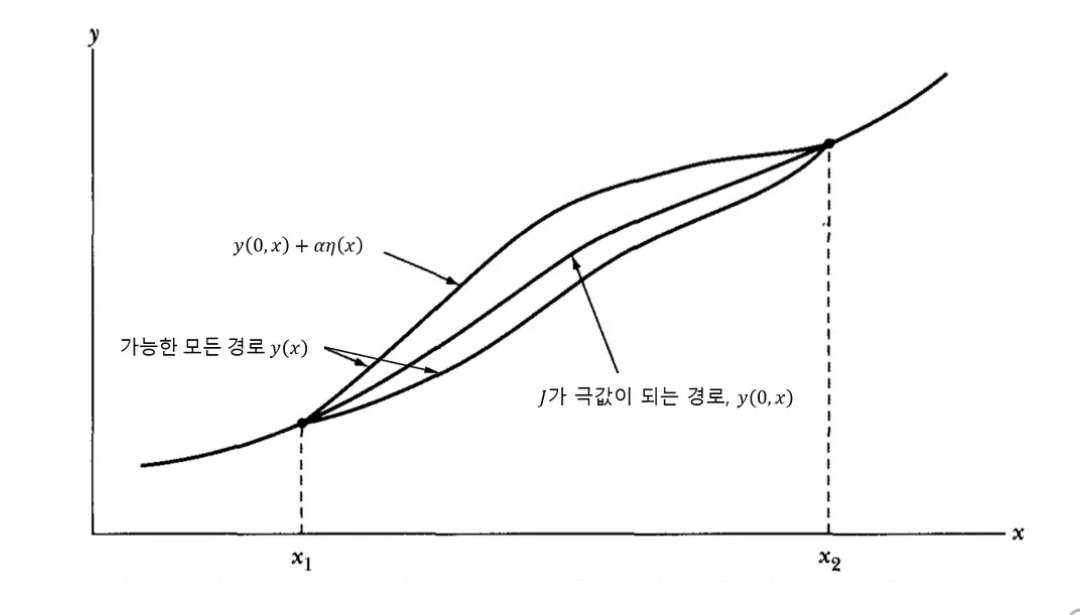
\includegraphics[width=0.7\linewidth]{figure5.1.jpg}
    \caption{범함수 $J$가 극값을 가지도록 하는 함수 $y(x)$의 그래프이다. 이웃한 함수 $y(0, x) + \alpha \eta(x)$의 그래프 역시 나타나 있다.}
    \label{fig:5.1}
\end{figure}

이제 $J$는 $\alpha$에 대한 함수가 되었다. $J$는 $\alpha = 0$에서 극값을 가지므로
\begin{equation}
    {\left.\dfrac{\partial J}{\partial\alpha}\right|}_{\alpha = 0} = 0
\end{equation}
을 만족해야 한다. 그런데 $J$의 $\alpha$에 대한 편미분은
\begin{equation}
    \frac{\partial J}{\partial \alpha} = \frac{\partial}{\partial \alpha} \int_{x_1}^{x_2} f(y, y' ; x) \mathrm{d}x
\end{equation}
이고, 적분 기호의 위끝과 아래끝이 상수이므로 편미분을 적분 안에 집어넣으면
\begin{equation}
    \frac{\partial J}{\partial \alpha} = \int_{x_1}^{x_2} \left(\frac{\partial f}{\partial y} \frac{\partial y}{\partial \alpha} +  \frac{\partial f}{\partial y'} \frac{\partial y'}{\partial \alpha} \right) \mathrm{d}x
\end{equation}
처럼 쓸 수 있다.\footnote{$x$의 $\alpha$에 대한 편미분은 0임을 유의하라.} 이때 식 \ref{eq:5.6}에 의해
\begin{equation}
    \begin{aligned}
        \frac{\partial y}{\partial \alpha} = \eta(x), \quad  \frac{\partial y'}{\partial \alpha} = \eta'(x)
    \end{aligned}
\end{equation}
이므로, 대입하여
\begin{equation}
    \frac{\partial J}{\partial \alpha} = \int_{x_1}^{x_2} \left( \frac{\partial f}{\partial y} \eta(x) +  \frac{\partial f}{\partial y'} \eta'(x) \right) \mathrm{d}x
\end{equation}
를 얻는다. 괄호 안의 두 번째 항을 부분적분하면
\begin{equation}
    \begin{aligned}
        \frac{\partial J}{\partial \alpha} &= \int_{x_1}^{x_2} \frac{\partial f}{\partial y} \eta(x)\mathrm{d}x+ \left[\frac{\partial f}{\partial y'} \eta(x) \right]_{x_1}^{x_2} - \int_{x_1}^{x_2} \frac{\mathrm{d}}{\mathrm{d}x} \left(\frac{\partial f}{\partial y'} \right) \eta(x) \mathrm{d}x \\
        &=\int_{x_1}^{x_2} \left(\frac{\partial f}{\partial y}-\frac{\mathrm{d}}{\mathrm{d}x}\frac{\partial f}{\partial y'} \right) \eta(x) \mathrm{d}x
    \end{aligned}
    \label{eq:5.12}
\end{equation}
가 된다. $\eta(x_1)=\eta(x_2) =0$이므로 우변의 가운데 항은 0이 됨을 유의하라. 이제 $J$가 극값을 가지려면, 변분법의 기본 보조정리에 따라
\begin{equation*}
    \frac{\partial f}{\partial y} - \frac{\mathrm{d}}{\mathrm{d}x}\frac{\partial f}{\partial y'} = 0
\end{equation*}
가 성립한다. 이는 식 \ref{eq:5.5}에서 본 오일러-라그랑주 방정식이다.

\begin{examplebox}{예제 5.1}
\begin{example}
평면 상의 두 점을 잇는 가장 짧은 경로는 직선임을 보여라.
\end{example}
\end{examplebox}

\begin{solution}
    평면 상의 두 점을 각각 $(x_1, y_1), (x_2, y_2)$로 두자. 경로의 미소 거리는 $\textrm{d}s = \sqrt{{\mathrm{d}x}^2 + {\mathrm{d}y}^2} = \sqrt{1 + {y'}^2} \ \mathrm{d}x$이므로, 경로의 총 거리 $l$은
    \begin{equation}
        l = \int_{x_1}^{x_2} \sqrt{1 + {y'}^2} \ \mathrm{d}x
    \end{equation}
    이다. 피적분함수를 $f$라고 하자. 오일러-라그랑주 방정식을 적용하면
    \begin{equation}
        \frac{y'}{\sqrt{1 + {y'}^2}} = C
        \label{eq:5.14}
    \end{equation}
    가 된다. 이때 $C$는 임의의 상수이다. 식 \ref{eq:5.14}를 정리하면
    \begin{equation}
        y' = \pm\sqrt{\frac{C^2}{1-C^2}}
    \end{equation}
    이고, 이 역시 상수이므로 $a$로 두면 적분하여
    \begin{equation}
        y = ax+b
        \label{eq:5.16}
    \end{equation}
    를 얻는다. 이는 직선의 방정식이다. $y(x_1) = y_1, y(x_2) = y_2$를 대입하여 $a$와 $b$의 값을 결정하면, 식 \ref{eq:5.16}은 두 점 사이를 지나는 직선임을 알 수 있다.
\end{solution}

\noindent\rule{\textwidth}{0.8pt} % 본문 전체 너비만큼 0.8pt 두께의 검은 줄을 긋습니다.
\vspace{1em} % 줄 아래에 약간의 여백을 줍니다.

\begin{examplebox}{예제 5.2}
\begin{example}
평면 상의 두 점 $(x_1, y_1$)와 $(x_2, y_2)$를 이은 곡선이 있다. 이 곡선을 $x$축을 중심으로 회전시켜 회전체를 만들 때, 회전체의 겉넓이가 최소가 되게 하는 곡선의 경로를 찾아라.
\end{example}
\end{examplebox}

\begin{solution}
    회전체의 겉넓이 $S$는 다음과 같다.
    \begin{equation}
        S = 2\pi \int_{x_1}^{x_2}y\sqrt{1+{y'}^2} \mathrm{d}x
        \label{eq:5.17}
    \end{equation}
    이제 피적분함수를 $f$로 잡고 오일러-라그랑주 방정식을 풀어도 되지만, 이 문제는 더 쉬운 풀이가 있다. 적분 변수를 $x$에서 $y$로 바꾸자. 그러면
    \begin{equation}
        S(x, x' ; y) = 2\pi \int_{y_1}^{y_2}y\sqrt{1+{x'}^2} \mathrm{d}y
    \end{equation}
    이다. 이제 이 식의 피적분함수를 $f$로 잡고 오일러-라그랑주 방정식을 적용하면
    \begin{equation}
        \frac{x'y}{\sqrt{1 + {x'}^2}} = C
        \label{eq:5.19}
    \end{equation}
    가 된다. 이때 $C$는 임의의 상수이다. 식 \ref{eq:5.19}를 정리하면
    \begin{equation}
    \begin{aligned}
        x' &= \frac{C}{\sqrt{y^2-C^2}} \\
        x &= \int\frac{C}{\sqrt{y^2-C^2}} \mathrm{d}y \\
        x &= C\cosh^{-1}{\left( \frac{y}{C} \right)} + D
    \end{aligned}
    \end{equation}
    를 얻는다. 이때 $D$는 적분 상수이다. 따라서 곡선은
    \begin{equation}
        y = C\cosh{\left( \frac{x-D}{C} \right)}
    \end{equation}
    이고, 이는 현수선(catenary)의 방정식이다.

    현수선은 줄의 퍼텐셜 에너지를 최소화하는 경로로도 알려져 있다. 줄의 선밀도를 $\rho$라고 하자. 미소 구간 $\mathrm{d}s$에서 줄의 퍼텐셜 에너지는 $\mathrm{d}U = \rho g y \mathrm{d}s$이므로, 퍼텐셜 에너지를 최소화하는 경로를 찾으려면 이 예제를 그대로 풀면 된다. 단지 계수 $2\pi$가 $\rho g$로 바뀔 뿐이다.
\end{solution}

\noindent\rule{\textwidth}{0.8pt} % 본문 전체 너비만큼 0.8pt 두께의 검은 줄을 긋습니다.
\vspace{1em} % 줄 아래에 약간의 여백을 줍니다.

만약 범함수 $J$가
\begin{equation}
    J = \int_{x_1}^{x_2} f(y_i (x), y'_i(x) ; x) \mathrm{d}x \quad (i=1, 2, \dots, n)
    \label{eq:5.22}
\end{equation}
처럼 $y_i$와 $y'_i$에 대한 다변수함수인 경우에도 오일러-라그랑주 방정식이 성립한다. 이때는 각 변수 $y_i, y'_i$에 대해 오일러-라그랑주 방정식을 적용하여
\begin{equation}
    \frac{\partial f}{\partial y_i} - \frac{\mathrm{d}}{\mathrm{d}x}\frac{\partial f}{\partial y'_i} = 0
\end{equation}
의 연립방정식을 풀면 된다.

\section{벨트라미 항등식 (Beltrami Identity)}
만약 $f$가 $y$와 $y'$만의 함수라면 우리는 오일러-라그랑주 방정식을 변형하여 문제를 쉽게 풀 수 있다. $f$의 전미분
\begin{equation}
    \frac{\mathrm{d}f}{\mathrm{d}x} = \frac{\partial f}{\partial y}\frac{\mathrm{d}y}{\mathrm{d}x} + \frac{\partial f}{\partial y'}\frac{\mathrm{d}y'}{\mathrm{d}x} + \frac{\partial f}{\partial x} = y'\frac{\partial f}{\partial y} + y''\frac{\partial f}{\partial y'} + \frac{\partial f}{\partial x}
\end{equation}
를 생각하자. 이때
\begin{equation*}
    \frac{\mathrm{d}}{\mathrm{d}x} \left( y' \frac{\partial f}{\partial y'} \right) = y"\frac{\partial f}{\partial y'} + y' \frac{\mathrm{d}}{\mathrm{d}x}\frac{\partial f}{\partial y'}
\end{equation*}
이므로
\begin{equation}
    \frac{\mathrm{d}}{\mathrm{d}x} \left( y' \frac{\partial f}{\partial y'} \right) = \frac{\mathrm{d}f}{\mathrm{d}x} - \frac{\partial f}{\partial x} - y'\frac{\partial f}{\partial y} + y' \frac{\mathrm{d}}{\mathrm{d}x}\frac{\partial f}{\partial y'}
\end{equation}
이다. 그런데 우변의 마지막 두 항을 $y'$으로 묶으면 오일러-라그랑주 방정식의 형태가 되므로 이는 0이다. 나머지를 정리하면
\begin{equation}
    \frac{\partial f}{\partial x} =  \frac{\mathrm{d}}{\mathrm{d}x} \left(f- y' \frac{\partial f}{\partial y'} \right)
\end{equation}
를 얻는다. 만약 $f$가 $x$에 명시적으로 의존하지 않는다면 $(\partial f / \partial x) =0$이므로
\begin{equation}
    f- y' \frac{\partial f}{\partial y'} = const.
\end{equation}
이다. 이는 \textbf{벨트라미 항등식(Beltrami Identity)}으로 알려져 있다.\footnote{벨트라미 항등식의 좌변은 $f$를 $y'$에 대해 르장드르 변환한 것이다. 또 $f$에 라그랑지안을 대입하면 이는 해밀토니안의 정의가 된다.} 많은 경우 벨트라미 항등식은 오일러-라그랑주 방정식보다 더 쉬운 풀이를 제공한다.

\begin{examplebox}{예제 5.3}
\begin{example}
원점에 정지해 있던 물체가 +y축 방향으로 균일한 크기의 중력 $mg$를 받으며 점 $(x_1, y_1$)으로 낙하한다. 물체가 최소 시간으로 낙하하는 경로, 즉 최속강하곡선(brachistochrone)을 구하여라.
\end{example}
\end{examplebox}

\begin{solution}
    시간은 거리 나누기 속력이다. 거리는 예제 5.1에서 구했듯 미소 거리 $\mathrm{d}s$의 적분으로 나타낼 수 있다. 한편 속력의 경우, 에너지 보존 법칙을 통해
    \begin{equation}
        \frac{1}{2}mv^2 = mgy \implies v = \sqrt{2gy}
    \end{equation}
   로 쓸 수 있다. $y$축의 방향에 유의하라. 따라서 시간 $t$는 다음과 같다.
    \begin{equation}
        t = \frac{1}{\sqrt{2g}} \int_0^{x_1} \sqrt{\frac{1+{y'}^2}{y}} \mathrm{d}y
        \label{eq:5.29}
    \end{equation}
    피적분함수를 $f$라고 하자. $f$가 $x$에 명시적으로 의존하지 않으므로 벨트라미 항등식을 적용하면
    \begin{equation}
        \frac{1}{\sqrt{y}\sqrt{1+{y'}^2}} = C
        \label{eq:5.30}
    \end{equation}
    가 된다. 이때 $C$는 임의의 상수이다. 식 \ref{eq:5.30}을 정리하면
    \begin{equation}
        \begin{aligned}
            1+{y'}^2 &= \frac{1}{C^2 y} \\
            \frac{\mathrm{d}y}{\mathrm{d}x} &= \sqrt{\frac{1-C^2 y}{C^2 y}} \\
            \frac{\mathrm{d}x}{\mathrm{d}y} &= \sqrt{\frac{C^2 y}{1-C^2 y}} \\
            x &= \int \sqrt{\frac{C^2 y}{1-C^2 y}} \mathrm{d}y
        \end{aligned}
    \end{equation}
    이다. 물체가 $+y$축 방향으로 낙하하므로 $y'$의 부호는 양수로 잡았다. 이 식을 적분할 수 있을까? 제곱근 안의 분자와 분모를 더하면 1이 된다는 사실을 고려하면, 우리는 변수 치환
    \begin{equation*}
        y \equiv \frac{\sin^2{(\theta/2)}}{C^2}, \quad \mathrm{d}y = \frac{\sin{(\theta/2)}\cos{(\theta/2)}}{C^2}\mathrm{d}\theta
    \end{equation*}
        을 이용하여
    \begin{equation}
        x = \int \frac{\sin{(\theta/2)}}{\cos{(\theta/2)}} \cdot \frac{\sin{(\theta/2)}\cos{(\theta/2)}}{C^2}\mathrm{d}\theta = \frac{1}{2C^2} \int (1-\cos{\theta})\mathrm{d}\theta
    \end{equation}
    를 얻을 수 있다. $x(\theta)$는 이 적분을 통해 구할 수 있으며, 물체의 출발점이 원점이므로 적분 상수는 간단히 $0$이 된다. 한편 $y(\theta)$는 변수 치환을 통해 바로 얻을 수 있고, 따라서 경로는 다음과 같다.
    \begin{equation}
    \begin{aligned}
        x &= a(\theta-\sin{\theta}) \\
        y &= a(1-\cos{\theta})
    \end{aligned}
    \label{eq:5.33}
    \end{equation}
    여기서 $a$는 $a\equiv 1/2C^2$으로 정의되는 상수이다. 이 식은 사이클로이드(cycloid)의 형태이다. 즉, 물체의 최속강하곡선은 사이클로이드의 일부이다.

    최속강하곡선 문제는 벨트라미 항등식을 쓰는 풀이가 그렇지 않은 풀이보다 더 쉽다. 벨트라미 항등식을 쓰지 않으면서 쉬운 풀이에 진입하고 싶다면, 좌표축을 바꾸어 속도를 $v=\sqrt{2gx}$로 나타내는 것을 추천한다.
\end{solution}

\noindent\rule{\textwidth}{0.8pt} % 본문 전체 너비만큼 0.8pt 두께의 검은 줄을 긋습니다.
\vspace{1em} % 줄 아래에 약간의 여백을 줍니다.

\begin{examplebox}{예제 5.4}
\begin{example}
우리는 예제 5.3에서 사이클로이드가 최속강하곡선임을 보였다. 이제 사이클로이드가 등시강하곡선(tautochrone)임을 보여라. 즉, 곡선 위에서 물체의 시작점이 어디든 그 물체가 최하점에 도달하는 시간이 같음을 보여라.
\end{example}
\end{examplebox}

\begin{solution}
    물체의 시작점을 $(x_0, y_0)$라고 하자. 사이클로이드 위의 임의의 점 $(x, y)$에서 물체의 속력은 에너지 보존 법칙에 의해
    \begin{equation}
        \frac{1}{2}mv^2 = mg(y-y_0) \implies v = \sqrt{2g(y-y_0)} = \sqrt{2ga (\cos{\theta_0} - \cos{\theta})}
    \end{equation}
    로 쓸 수 있다. 한편 식 \ref{eq:5.33}을 이용하면 미소 거리는 $\mathrm{d}s = 2a\sin{(\theta/2)}\mathrm{d}\theta$이므로, 시간 $t$는 다음과 같다.
    \begin{equation}
    \begin{aligned}
        t &= \sqrt{\frac{2a}{g}} \int_{\theta_0}^{\pi} \frac{\sin{(\theta/2)}}{\sqrt{\cos{\theta_0} - \cos{\theta}}}\mathrm{d}\theta
    \end{aligned}
    \label{eq:5.35}
    \end{equation}
    이제 변수 치환
    \begin{equation*}
        u \equiv \cos{(\theta/2)}, \quad \mathrm{d}u = -\frac{1}{2}\sin{(\theta/2)}\mathrm{d}\theta
    \end{equation*}
    을 적용하면 식 \ref{eq:5.35}는
    \begin{equation}
    \begin{aligned}
        t &= \sqrt{\frac{a}{g}} \int_{u_0}^{0} \frac{-2}{\sqrt{{u_0}^2-{u}^2}}\mathrm{d}\theta = \sqrt{\frac{a}{g}} \int_{0}^{u_0} \frac{2}{\sqrt{{u_0}^2-{u}^2}}\mathrm{d}\theta \\
        &= {\left.2\sqrt{\frac{a}{g}} \sin^{-1}{\left(\frac{u}{u_0}\right)} \right|}_0^{u_0} = \pi \sqrt{\frac{a}{g}}
    \end{aligned}
    \label{eq:5.37}
    \end{equation}
    처럼 풀린다. 적분 과정에서 시작점과 관련된 항이 모두 사라졌음을 보라. 이는 사이클로이드 상에서 물체의 시작점이 어디든 그 물체가 최하점까지 가는 데 걸리는 시간이 같음을 의미한다.
\end{solution}

\noindent\rule{\textwidth}{0.8pt} % 본문 전체 너비만큼 0.8pt 두께의 검은 줄을 긋습니다.
\vspace{1em} % 줄 아래에 약간의 여백을 줍니다.

\begin{examplebox}{예제 5.5}
\begin{example}
측지선(geodesic)은 어떤 평면 상에 있는 두 점 사이의 최단 경로를 나타낸다. 구면의 측지선을 구하여라.
\end{example}
\end{examplebox}

\begin{solution}
    $(r, \phi, \theta)$의 구면좌표계를 활용하자. 구면 위에선 $\mathrm{d}r = 0$이므로, 구면의 반지름을 $\rho$로 잡으면 구면의 미소 길이는
    \begin{equation}
        \mathrm{d}s = \sqrt{\rho^2({\mathrm{d}\theta}^2 + \sin^2{\theta}{\mathrm{d}\phi}^2)}
    \end{equation}
    로 나타낼 수 있다. 따라서 점 1과 점 2 사이의 거리 $s$는
    \begin{equation}
        s(\theta, \theta' ; \phi) = \int_1^2 \sqrt{{\left( \frac{\mathrm{d}\theta}{\mathrm{d}\phi}\right)}^2 + \sin^2{\theta}} \ \mathrm{d}\phi = \int_1^2 \sqrt{{\theta'}^2 + {\sin}^2{\theta}} \ \mathrm{d}\phi 
    \end{equation}
    이다. 만약 $s$가 최솟값을 가진다면, 함수 $f = \sqrt{(\theta'^2 + \sin^2{\theta})}$는 벨트라미 항등식에 따라
    \begin{equation}
        \sqrt{({\theta'}^2 + \sin^2{\theta})} - \theta' \cdot \frac{\partial}{\partial\theta'}\sqrt{({\theta'}^2 + \sin^2{\theta})} = C
        \label{eq:5.39}
    \end{equation}
    를 만족해야 한다. 이때 $C$는 임의의 상수이다. 식 \ref{eq:5.39}를 풀면 다음과 같다.
    \begin{equation}
    \begin{aligned}
        \sqrt{({\theta'}^2 + \sin^2{\theta})} - {\theta'}^2 \frac{1}{ \sqrt{({\theta'}^2 + \sin^2{\theta})}} &= C \\
         ({\theta'}^2 + \sin^2{\theta}) - {\theta'}^2 &= C\sqrt{({\theta'}^2 + \sin^2{\theta})} \\
         \sin^2{\theta} &= C\sqrt{({\theta'}^2 + \sin^2{\theta})} \\
         {\theta'}^2 &= \frac{\sin^2{\theta}(\sin^2{\theta}-C^2)}{C^2} \\
         \mathrm{d}\phi &= \frac{C \mathrm{d}\theta}{\sin{\theta} \sqrt{\sin^2{\theta}-C^2}}
    \end{aligned}
    \end{equation}
    변수 치환
    \begin{equation*}
        \cot{\theta} \equiv u, \quad -\csc^2{\theta}\mathrm{d}\theta = \mathrm{d}u, \quad \mathrm{d}\theta = -\frac{1}{1+u^2} \mathrm{d}u
    \end{equation*}
    을 이용하면 위 식은
    \begin{equation}
        \begin{aligned}
            \mathrm{d}\phi &= \frac{-C\mathrm{d}u}{\sqrt{1-C^2-C^2u^2}}
        \end{aligned}
    \end{equation}
    로 바뀌고, 다시 변수 치환
    \begin{equation*}
        A \equiv \sqrt{1-C^2}, \quad w \equiv \frac{Cu}{A}, \quad \mathrm{d}w = \frac{C}{A} \mathrm{d}u
    \end{equation*}
    을 적용하면
    \begin{equation}
        \phi = -\int \frac{A \mathrm{d}w}{A\sqrt{1-w^2}} = -\int \frac{\mathrm{d}w}{\sqrt{1-w^2}} = -\sin^{-1}{w} + \phi_0
        \label{eq:5.42}
    \end{equation}
    를 얻는다. 이때 $\phi_0$는 적분 상수이다. 식 \ref{eq:5.42}를 정리하면
    \begin{equation}
        \begin{aligned}
            \frac{C}{\sqrt{1-C^2}} \cot{\theta} &= \sin{(\phi_0 - \phi)} \\
            \cot{\theta} &= K\sin{(\phi_0 - \phi)}
        \end{aligned}
    \end{equation}
    가 된다. 이때 $K$는 $K \equiv (\sqrt{1-C^2} / C^2)$으로 정의되는 상수이다. 구면좌표계를 직교좌표계로 바꾸기 위해 양변에 $r\sin{\theta}$를 곱하면
    \begin{equation}
    \begin{aligned}
        r\cos{\theta} &= Kr\sin{\theta}\sin{(\phi_0 - \phi)} \\
        r\cos{\theta} &= Kr\sin{\theta}(\sin{\phi_0}\cos{\phi} - \cos{\phi_0}\sin{\phi}) \\
        z &= K(x\sin{\phi_0}-y\cos{\phi_0})
    \end{aligned}
    \end{equation}
    를 얻는다. 이는 원점을 지나는 평면의 방정식이다. 문제의 조건에 따라 곡선은 구면 위에 놓여 있으므로, 측지선은 원점을 지나는 평면과 구면의 교선인 \textbf{대원(great circle)}이 된다. 구면의 측지선은 비행기의 최적 항로 등을 잘 설명한다.
\end{solution}

\noindent\rule{\textwidth}{0.8pt} % 본문 전체 너비만큼 0.8pt 두께의 검은 줄을 긋습니다.
\vspace{1em} % 줄 아래에 약간의 여백을 줍니다.

\begin{examplebox}{예제 5.6}
\begin{example}
페르마의 원리(Fermat's principle)에 따르면 빛은 두 점 사이를 이동할 때 광행시간이 최소가 되는 경로를 따른다. 굴절률이 각각 $n_1, n_2$인 두 균일한 매질이 $x$축에 평행한 경계면을 사이에 두고 있을 때, 변분법을 통해 페르마의 원리를 확인하고 스넬의 법칙(Snell's law)을 유도하라.
\end{example}
\end{examplebox}

\begin{solution}
    빛이 $\mathbb{R}^2$ 평면에서 이동하고, 빛의 궤적이 어떠한 함수 $y$의 그래프를 따라간다고 가정하자. 매질에서의 빛의 속도를 고려하면, 미소 거리 $\mathrm{d}s$를 지날 때 걸리는 미소 시간은 다음과 같다.
    \begin{equation}
        \mathrm{d}t = \frac{n(y)\mathrm{d}s}{c}
    \end{equation}
    이때 $c$는 진공에서의 빛의 속도이며 $n(y)$는 $y$에서의 굴절률이다. 따라서 점 1에서 점 2까지 빛이 이동하는 데 걸리는 시간은
    \begin{equation}
        t = \frac{1}{c} \int_1^2 n(y) \sqrt{1+{y'}^2} \mathrm{d}y
    \end{equation}
    이다. 피적분함수를 $f$로 두자. $f$는 $x$에 명시적으로 의존하지 않으므로, 만약 $f$가 최솟값을 가진다면 벨트라미 항등식에 따라
    \begin{equation}
        n(y)\sqrt{1+{y'}^2} - y' \frac{n(y)y'}{\sqrt{1+{y'}^2}} = const.
        \label{eq:5.47}
    \end{equation}
    를 만족해야 한다. 식 \ref{eq:5.47}을 풀면 다음과 같다.
    \begin{equation}
        \frac{n(y)}{\sqrt{1+{y'}^2}} = const.
        \label{eq:5.48}
    \end{equation}
    이때 빛의 진행 경로 상의 한 점이 법선과 이루는 각도를 $\theta$라고 한다면, 법선은 $y$축이므로 기울기 $y'$은
    \begin{equation}
        y' = \tan{\left(\frac{\pi}{2}-\theta \right)} = \cot{\theta}
    \end{equation}
    을 만족한다. 이를 식 \ref{eq:5.48}에 대입하면
    \begin{equation}
        n(y)\sin{\theta} = const. 
    \end{equation}
    이므로 다음과 같은 스넬의 법칙을 얻는다.
    \begin{equation}
         n_1\sin{\theta_1} = n_2\sin{\theta_2}
    \end{equation}
\end{solution}

\noindent\rule{\textwidth}{0.8pt} % 본문 전체 너비만큼 0.8pt 두께의 검은 줄을 긋습니다.
\vspace{1em} % 줄 아래에 약간의 여백을 줍니다.

\section{구속 방정식 (Equations of Constraint)}
구속 조건 혹은 \textbf{구속 방정식(equations of constraint)}이 주어진 경우 오일러-라그랑주 방정식을 푸는 법을 조사하자. 이때 구속 방정식이라 함은 문제 상황에서 경로가 만족해야 할 조건을 나타낸 것이며, 예제 5.5로 예를 들면
\begin{equation}
    x^2 + y^2+z^2 = r^2
    \label{eq:5.52}
\end{equation}
가 될 것이다.

우리는 미적분학 시간에 \textbf{라그랑주 승수법(Lagrange multipliers)}에 관해 배웠다. 정확히 같은 논리가 이 절에도 적용된다. 우선, 구속 방정식의 우변의 값이 0이 되도록 함수 $g$를 잡자. 식 \ref{eq:5.52}로 예를 들면
\begin{equation}
    g : x^2 + y^2 + z^2 - r^2 = 0
\end{equation}
처럼 말이다. 우리가 풀고자 하는 문제는 $g=0$일 때이므로 
\begin{equation}
    \tilde{J} = \int_{x_1}^{x_2} [f(y, y' ;x) + \lambda(x)g(y, y' ;x)] \mathrm{d}x
    \label{eq:5.54}
\end{equation}
와 같이 새로운 범함수 $\tilde{J}$를 정의한 다음 이것의 오일러-라그랑주 방정식을 풀면 된다. 새로운 함수 $F=f+\lambda g$를 생각하라. 여기서 $\lambda(x)$는 아직 정해지지 않은 함수이다. 식 \ref{eq:5.54}에 $g=0$을 대입하면 이는 원래 문제와 같음을 알 수 있다.

$\tilde{J}$가 극값을 가진다면 $F$는 오일러-라그랑주 방정식을 만족해야 하므로, 이를 풀면
\begin{equation}
    \frac{\partial f}{\partial y} - \frac{\mathrm{d}}{\mathrm{d}x}\frac{\partial f}{\partial y'} + \lambda(x)\frac{\partial g}{\partial y} - \frac{\mathrm{d}}{\mathrm{d}x} \left(\lambda(x)\frac{\partial g}{\partial y'} \right) = 0
\end{equation}
을 얻는다. 이것이 끝이다. 특히 많은 문제에선 $g$가 $y'$에 의존하지 않으므로\footnote{이를 홀로노믹 구속 조건(holonomic constraint)이라고 한다. 일반적으로 홀로노믹 구속 조건은 위치 $y$와 독립변수 $x$만으로 표현되는 구속 조건을 말한다. 다만 속도 $y'$에 의존하는 구속 조건도 적분 가능하다면 홀로노믹일 수 있다. 이 용어는 6장과 7장에서 다시 등장할 것이다.}
\begin{equation}
     \frac{\partial f}{\partial y} - \frac{\mathrm{d}}{\mathrm{d}x}\frac{\partial f}{\partial y'} + \lambda(x)\frac{\partial g}{\partial y} = 0
\end{equation}
가 성립한다. 이것이 바로 일반형 구속 방정식이 주어진 오일러-라그랑주 방정식의 형태이다. 여기서 $\lambda(x)$는 라그랑주 승수의 역할을 한다.

만약 $g_j=0$인 $m$개의 구속 방정식에 대해, 범함수 $\tilde{J}$가
\begin{equation}
    \tilde{J} = \int_{x_1}^{x_2} \left[f(y_i (x), y'_i(x) ; x) + \sum_{j=1}^{m}\lambda_j(x)g_j(y_i (x), y'_i(x) ; x) \right] \mathrm{d}x
    \label{eq:5.57}
\end{equation}
처럼 $y_i$와 $y'_i$에 대한 다변수함수인 경우에도 오일러-라그랑주 방정식이 성립한다. 이때는 각 변수 $y_i, y'_i$에 대해 오일러-라그랑주 방정식을 적용하여
\begin{equation}
\begin{aligned}
    \frac{\partial f}{\partial y_i} - \frac{\mathrm{d}}{\mathrm{d}x}\frac{\partial f}{\partial y'_i} + \sum_{j=1}^{m}\lambda_j(x)\frac{\partial g_j}{\partial y_i} - \frac{\mathrm{d}}{\mathrm{d}x} \left(\sum_{j=1}^{m}\lambda_j(x)\frac{\partial g_j}{\partial y'_i} \right) = 0 \\
    g_j(y_i, y'_i ; x) = 0
\end{aligned}
\label{eq:5.58}
\end{equation}
의 연립방정식을 풀면 된다. $i=1, 2, \dots, n$이고 $j=1, 2, \dots, m$임을 유의하라. 항상 그렇지는 않지만, 우리는 보통 식 \ref{eq:5.58}의 윗줄로부터 $n$개의 정보를, 아랫줄로부터 $m$개의 정보를 얻어 총 $m+n$개의 미지수를 결정할 수 있다. 만약 $g_j$가 $y'$에 의존하지 않는다면 이 식은
\begin{equation}
\begin{aligned}
    \frac{\partial f}{\partial y_i} - \frac{\mathrm{d}}{\mathrm{d}x}\frac{\partial f}{\partial y'_i} + \sum_{j=1}^{m}\lambda(x)_j\frac{\partial g_j}{\partial y_i} = 0 \\
    g_j(y_i, y'_i ; x) = 0
\end{aligned}
\label{eq:5.59}
\end{equation}
와 같이 간단해진다. 추가적으로 $g_j$를 전미분하면
\begin{equation}
    \mathrm{d}g = \sum_{j=1}^{m} \frac{\partial g_j}{\partial y_i} \mathrm{d}y_i + \frac{\partial g_j}{\partial x} \mathrm{d}x
\end{equation}
이고, 변분은 $x$를 고정했을 때 $y_i$가 바뀜에 따라 $g$가 어떻게 바뀌는지를 확인하는 것이므로 $\mathrm{d}x = 0$이다. 이때 $g=0$이므로 결국
\begin{equation}
    \mathrm{d}g = \sum_{j=1}^{m} \frac{\partial g_j}{\partial y_i} \mathrm{d}y_i = 0
\end{equation}
이 성립한다. 이는 구속 방정식이 미분방정식인 경우 식 \ref{eq:5.59}의 아랫줄을 푸는 것보다 종종 더 간단한 풀이를 제공한다.

\begin{examplebox}{예제 5.7}
\begin{example}
장반경이 $a$, 단반경이 $b$인 타원이 있다. 이 타원에 내접하는 직사각형 중 넓이가 최대인 직사각형을 찾아라.
\end{example}
\end{examplebox}

\begin{solution}
    타원의 중심을 원점으로 잡자. 직사각형과 타원이 만나는 제1사분면 상의 점을 $(x, y)$로 두면, 대칭성에 따라 직사각형의 넓이는 $f=4xy$가 된다. 이제 구간 $t \in [0, 1]$에서 $x, y$를 상수함수로 생각하고 범함수 $J$를 다음과 같이 정의하자.
    \begin{equation}
        J = \int_0^1 4x(t)y(t)\mathrm{d}t 
    \end{equation}
    다음으로 구속 방정식 $g$는 $g:(x/a)^2 + (y/b)^2 - 1 = 0$을 만족한다. 따라서 일반형 구속 조건이 주어진 오일러-라그랑주 방정식
    \begin{equation}
        \begin{aligned}
            \frac{\partial f}{\partial x} - \frac{\mathrm{d}}{\mathrm{d}t}\frac{\partial f}{\partial x'} + \lambda(t)\frac{\partial g}{\partial x} = 0 \\
            \frac{\partial f}{\partial y} - \frac{\mathrm{d}}{\mathrm{d}t}\frac{\partial f}{\partial y'} + \lambda(t)\frac{\partial g}{\partial y} = 0
        \end{aligned}
    \end{equation}
    을 풀면, 우리는 다음과 같은 연립방정식을 얻는다.
    \begin{equation}
        \begin{aligned}
            4y + \frac{2\lambda x}{a^2} = 0 \\
            4x + \frac{2\lambda y}{b^2} = 0 \\
            \frac{x^2}{a^2} + \frac{y^2}{b^2} - 1 = 0
        \end{aligned}
    \end{equation}
    이는 식 \ref{eq:5.59}와 정확히 대응된다. 연립방정식을 풀면 $x = (a/\sqrt{2}), y = (b/\sqrt{2})$를 얻고, 따라서 직사각형의 넓이는 $2ab$이다. 산술-기하평균 부등식에 의해 이 값은 최댓값을 보장한다. 이 문제는 라그랑주 승수법 $\nabla f + \lambda \nabla g = 0$ 을 푸는 것과 같다.
\end{solution}

\noindent\rule{\textwidth}{0.8pt} % 본문 전체 너비만큼 0.8pt 두께의 검은 줄을 긋습니다.
\vspace{1em} % 줄 아래에 약간의 여백을 줍니다.

한편 구속 방정식이 단순한 방정식의 형태가 아니라 적분형으로 주어질 수도 있다. 주로 길이나 넓이, 부피가 구속 조건으로 주어진 경우가 그렇다. 이 경우에도 방법은 같다. $g$를 우변이 0이 되도록 잡자. 구속 방정식
\begin{equation}
    \int_{x_1}^{x_2} h(y, y'; x) \mathrm{d}x = C
    \label{eq:5.65}
\end{equation}
에 대해
\begin{equation}
    g : \int_{x_1}^{x_2} h(y, y'; x) \mathrm{d}x - C = 0
    \label{eq:5.66}
\end{equation}
처럼 말이다. 우리가 풀고자 하는 문제는 $g=0$일 때이므로
\begin{equation}
    \tilde{J} = \int_{x_1}^{x_2} f(y, y' ;x)\mathrm{d}x + \lambda g(y, y';x)
    \label{eq:5.64}
\end{equation}
와 같이 새로운 범함수 $\tilde{J}$를 정의한 다음 이것의 오일러-라그랑주 방정식을 풀면 된다. 일반형 구속 방정식이 주어진 오일러-라그랑주 방정식을 구할 때와 달리 $g$를 적분 바깥에 더했지만, $g = 0$을 대입하면 이는 원래 문제와 같음을 알 수 있다. 이제 식을 정리하자.
\begin{equation}
    \begin{aligned}
        \tilde{J} &= \int_{x_1}^{x_2} f(y, y' ;x)\mathrm{d}x + \lambda\left[ \int_{x_1}^{x_2} h(y, y'; x) \mathrm{d}x - C\right] \\
        &= \int_{x_1}^{x_2} [f(y, y' ;x) + \lambda h(y, y';x) ]\mathrm{d}x - \lambda C
    \end{aligned}
\end{equation}
$\lambda C$는 $y$에 의존하지 않으므로 $y$에 대한 변분에 영향을 끼치지 않는다. 따라서 우리는 피적분함수를 $F=f+\lambda h$로 생각하고 오일러-라그랑주 방정식을 풀면 된다. 이를 풀면
\begin{equation}
    \frac{\partial f}{\partial y} - \frac{\mathrm{d}}{\mathrm{d}x}\frac{\partial f}{\partial y'} + \lambda \left(\frac{\partial h}{\partial y} - \frac{\mathrm{d}}{\mathrm{d}x} \frac{\partial h}{\partial y'} \right) = 0
    \label{eq:5.69}
\end{equation}
를 얻는다. 이것이 바로 적분형 구속 방정식이 주어진 오일러-라그랑주 방정식의 형태이다. 마찬가지로 여기서 $\lambda$는 라그랑주 승수의 역할을 한다.

\begin{examplebox}{예제 5.8}
\begin{example}
평면 위의 점 $(-a, 0)$과 $(a, 0)$을 잇는 길이 $l$인 곡선이 있다. 이 곡선이 $x$축과 이루는 영역의 넓이를 $A$라고 할 때, $A$의 최댓값을 구하여라.
\end{example}
\end{examplebox}

\begin{solution}
    미소 면적은 $\mathrm{d}A = y \mathrm{d}x$이다. 따라서 범함수 $A$는 다음과 같다.
    \begin{equation}
        A = \int_{-a}^{a} y \mathrm{d}x
    \end{equation}
    피적분함수 $y$를 $f$라고 하자. 다음으로 구속 방정식은
    \begin{equation}
        g : l = \int_{-a}^{a} \sqrt{1 + {y'}^2} \mathrm{d}x
    \end{equation}
    처럼 적분형으로 주어진다. 이제 적분형 구속 조건이 주어진 오일러-라그랑주 방정식을 풀면
    \begin{equation}
    \frac{\mathrm{d}}{\mathrm{d}x} \left[\frac{y'}{\sqrt{1 + y'^2}} \right] = \frac{1}{\lambda}
    \end{equation}
    을 얻는다. 식을 정리하면
    \begin{equation}
        \begin{aligned}
            \frac{\lambda y'}{\sqrt{1 + y'^2}} &= x-C_1 \\
            \mathrm{d}y &= \pm \frac{(x-C_1)\mathrm{d}x}{\sqrt{\lambda^2-{(x-C_1)}^2}} \\
            y &= \mp \sqrt{\lambda^2-{(x-C_1)}^2} + C_2
        \end{aligned}
        \label{eq:5.73}
    \end{equation}
    이다. 이때 $C_1, C_2$는 적분 상수이다. 식 \ref{eq:5.73}은
    \begin{equation}
        {(x-C_1)}^2 + {(y-C_2)}^2 = \lambda^2
    \end{equation}
    인 원의 방정식으로 쓸 수 있다. 즉, 주어진 구속 방정식 하에서 넓이를 최대로 만드는 도형은 반원이다. 반지름이 $\lambda = (l/\pi)$이므로 A의 최댓값은 $(l^2/2 \pi)$이다. 이 문제는 카르타고의 여왕 디도의 문제(Dido problem)로 알려져 있다.
\end{solution}

\noindent\rule{\textwidth}{0.8pt} % 본문 전체 너비만큼 0.8pt 두께의 검은 줄을 긋습니다.
\vspace{1em} % 줄 아래에 약간의 여백을 줍니다.

%여기서부터 overleaf 수정 필요, 2026-10-17$
\section{델타 표기법 (The Delta Notation)}
변분법을 나타낼 때, 우리는 관습적으로
\begin{equation}
    \delta y = \frac{\partial y}{\partial{\alpha}} \mathrm{d}\alpha
\end{equation}
처럼 $\delta$ 표기법을 사용한다. 이때 $\delta y$는 $y$의 변분(variation)이라고 한다. 변분은 미분과 비슷하지만, $\delta$는 $y$의 변화를 나타내며 $x$는 고정되어 있다. 즉, $\delta y(x)$는 $x$가 고정된 상태에서 $y$가 어떻게 변하는지를 나타낸다. 이는 우리가 변분을 정의할 때 사용한 개념과 일치한다.

변분을 통해 오일러-라그랑주 방정식을 다시 쓰자. 식 \ref{eq:5.12}의 양변에 $\mathrm{d}a$를 곱하고 $\eta(x) = \partial{y} / \partial{\alpha}$를 대입하면
\begin{equation}
    \delta J = \int_{x_1}^{x_2} \left(\frac{\partial f}{\partial y} - \frac{\mathrm{d}}{\mathrm{d}x}\frac{\partial f}{\partial y'}\right) \delta y \mathrm{d}x
\end{equation}
을 얻는다. 만약 $J$가 극값을 가진다면, $\delta J = 0$이므로 다음은 모두 동치가 된다.
\begin{equation}
    \delta J = 0 \iff \int_{x_1}^{x_2} \left(\frac{\partial f}{\partial y} - \frac{\mathrm{d}}{\mathrm{d}x}\frac{\partial f}{\partial y'}\right) \delta y \mathrm{d}x = 0 \iff \frac{\partial f}{\partial y} - \frac{\mathrm{d}}{\mathrm{d}x}\frac{\partial f}{\partial y'} = 0
\end{equation}
증명할 수도 있다. 함수 $f(y, y';x)$의 변분은
\begin{equation}
    \begin{aligned}
        \delta f &= \frac{\partial f}{\partial y} \frac{\partial y}{\partial \alpha} \mathrm{d}\alpha + \frac{\partial f}{\partial y'} \frac{\partial y'}{\partial \alpha} \mathrm{d}\alpha = \frac{\partial f}{\partial y} \delta y + \frac{\partial f}{\partial y'} \delta y' \\
    \end{aligned}
\end{equation}
이고
\begin{equation}
    \delta y' = \frac{\partial}{\partial x} \left(\frac{\partial y}{\partial \alpha} \mathrm{d}\alpha \right) = \frac{\partial}{\partial x} (\delta y) = (\delta y)'
\end{equation}
이므로 오일러-라그랑주 방정식은
\begin{equation}
    \begin{aligned}
    \delta J &= \int_{x_1}^{x_2} \delta f \mathrm{d}x =\int_{x_1}^{x_2} \left(\frac{\partial f}{\partial y} \delta y + \frac{\partial f}{\partial y'} (\delta y)' \right) \mathrm{d}x \\
    &= \int_{x_1}^{x_2} \left(\frac{\partial f}{\partial y} \delta y + \frac{\mathrm{d}}{\mathrm{d}x}\left[\frac{\partial f}{\partial y'} \delta y\right] - \frac{\mathrm{d}}{\mathrm{d}x}\frac{\partial f}{\partial y'} \delta y \right) \mathrm{d}x \\
    &= \int_{x_1}^{x_2} \left(\frac{\partial f}{\partial y} - \frac{\mathrm{d}}{\mathrm{d}x}\frac{\partial f}{\partial y'}\right) \delta y \mathrm{d}x + {\left. \frac{\partial f}{\partial y'} \delta y \right|}_{x_1}^{x_2} \\
    &= \int_{x_1}^{x_2} \left(\frac{\partial f}{\partial y} - \frac{\mathrm{d}}{\mathrm{d}x}\frac{\partial f}{\partial y'}\right) \delta y \mathrm{d}x
    \end{aligned}
\end{equation}
와 같이 얻어진다.

\newpage
% Chapter 6 시작
\chapter{라그랑주 역학 (Lagrangian Mechanics)}

\newpage
% Chapter 7 시작
\chapter{해밀턴 역학 (Hamiltonian Mechanics)}

\newpage
% Chapter 8 시작
\chapter{중심력과 천체역학 (Central Forces and Celestial Mechanics)}

\newpage
% Chapter 9 시작
\chapter{입자계의 운동역학 (Dynamics of a System of Particles)}


\end{document}